\documentclass[twoside,11pt]{article}

% ? Specify used packages
\usepackage{graphicx} % Use this one for final production.
% \usepackage[draft]{graphicx} % Use this one for drafting.
\usepackage{array}
\usepackage{fancyhdr}
\usepackage{multirow}
% ? End of specify used packages
\usepackage{longtable}
\usepackage{color}
\pagestyle{myheadings}

% -----------------------------------------------------------------------------

% ? Document identification
\newcommand{\stardoccategory} {Starlink Cookbook}
\newcommand{\stardocinitials} {SC}
\newcommand{\stardocsource} {sc\stardocnumber}
\newcommand{\stardoccopyright} {Copyright \copyright\ 2014 Science and Technology Facilities Council}
\newcommand{\stardocnumber} {21.2}
\newcommand{\stardocauthors} {H. S. Thomas}
\newcommand{\stardocdate} {11 June 2014}
\newcommand{\stardoctitle} {The SCUBA-2 Data Reduction Cookbook}
\newcommand{\stardocversion} {1.3}
\newcommand{\stardocmanual} {\ }
\newcommand{\stardocabstract} {

   This cookbook provides a short introduction to Starlink facilities,
   especially \textsc{Smurf}, the Sub-Millimetre User Reduction
   Facility, for reducing, displaying, and calibrating SCUBA-2 data.
   It describes some of the data artefacts present in SCUBA-2
   time-series and methods to mitigate them. In particular, this
   cookbook illustrates the various steps required to reduce the data;
   and gives an overview of the Dynamic Iterative Map-Maker, which
   carries out all of these steps using a single command controlled by
   a configuration file. Specialised configuration files are
   presented.}

% ? End of document identification

% -----------------------------------------------------------------------------

% +
%  Name:
%     sc.tex
%
% Purpose:
% Template for Starlink Cookbook (SC) documents.
% Refer to SUN/199
%
%  Authors:
%     AJC: A.J.Chipperfield (Starlink, RAL)
%     BLY: M.J.Bly (Starlink, RAL)
%     PWD: Peter W. Draper (Starlink, Durham University)
%
%  History:
%     16-JUN-1997 (BLY):
%        Original, based on SUN/SG templates.
%     13-AUG-1998 (PWD):
%        Converted for use with LaTeX2HTML version 98.2 and
%        Star2HTML version 1.3.
%      1-FEB-2000 (AJC):
%        Add Copyright statement in LaTeX
%     {Add further history here}
%
% -

\newcommand{\stardocname}{\stardocinitials /\stardocnumber}
\markboth{\stardocname}{\stardocname}
\setlength{\textwidth}{160mm}
\setlength{\textheight}{230mm}
\setlength{\topmargin}{-2mm}
\setlength{\oddsidemargin}{0mm}
\setlength{\evensidemargin}{0mm}
\setlength{\parindent}{0mm}
\setlength{\parskip}{\medskipamount}
\setlength{\unitlength}{1mm}

% -----------------------------------------------------------------------------
%  Hypertext definitions.
%  ======================
%  These are used by the LaTeX2HTML translator in conjunction with star2html.

%  Comment.sty: version 2.0, 19 June 1992
%  Selectively in/exclude pieces of text.
%
%  Author
%    Victor Eijkhout                                      <eijkhout@cs.utk.edu>
%    Department of Computer Science
%    University Tennessee at Knoxville
%    104 Ayres Hall
%    Knoxville, TN 37996
%    USA

%  Do not remove the %begin{latexonly} and %end{latexonly} lines (used by
%  LaTeX2HTML to signify text it shouldn't process).
%begin{latexonly}
\makeatletter
\def\makeinnocent#1{\catcode`#1=12 }
\def\csarg#1#2{\expandafter#1\csname#2\endcsname}

\def\ThrowAwayComment#1{\begingroup
    \def\CurrentComment{#1}%
    \let\do\makeinnocent \dospecials
    \makeinnocent\^^L% and whatever other special cases
    \endlinechar`\^^M \catcode`\^^M=12 \xComment}
{\catcode`\^^M=12 \endlinechar=-1 %
 \gdef\xComment#1^^M{\def\test{#1}
      \csarg\ifx{PlainEnd\CurrentComment Test}\test
          \let\html@next\endgroup
      \else \csarg\ifx{LaLaEnd\CurrentComment Test}\test
            \edef\html@next{\endgroup\noexpand\end{\CurrentComment}}
      \else \let\html@next\xComment
      \fi \fi \html@next}
}
\makeatother

\def\includecomment
 #1{\expandafter\def\csname#1\endcsname{}%
    \expandafter\def\csname end#1\endcsname{}}
\def\excludecomment
 #1{\expandafter\def\csname#1\endcsname{\ThrowAwayComment{#1}}%
    {\escapechar=-1\relax
     \csarg\xdef{PlainEnd#1Test}{\string\\end#1}%
     \csarg\xdef{LaLaEnd#1Test}{\string\\end\string\{#1\string\}}%
    }}

%  Define environments that ignore their contents.
\excludecomment{comment}
\excludecomment{rawhtml}
\excludecomment{htmlonly}

%  Hypertext commands etc. This is a condensed version of the html.sty
%  file supplied with LaTeX2HTML by: Nikos Drakos <nikos@cbl.leeds.ac.uk> &
%  Jelle van Zeijl <jvzeijl@isou17.estec.esa.nl>. The LaTeX2HTML documentation
%  should be consulted about all commands (and the environments defined above)
%  except \xref and \xlabel which are Starlink specific.

\newcommand{\htmladdnormallinkfoot}[2]{#1\footnote{#2}}
\newcommand{\htmladdnormallink}[2]{#1}
\newcommand{\htmladdimg}[1]{}
\newcommand{\hyperref}[4]{#2\ref{#4}#3}
\newcommand{\htmlref}[2]{#1}
\newcommand{\htmlimage}[1]{}
\newcommand{\htmladdtonavigation}[1]{}

\newenvironment{latexonly}{}{}
\newcommand{\latex}[1]{#1}
\newcommand{\html}[1]{}
\newcommand{\latexhtml}[2]{#1}
\newcommand{\HTMLcode}[2][]{}

%  Starlink cross-references and labels.
\newcommand{\xref}[3]{#1}
\newcommand{\xlabel}[1]{}

%  LaTeX2HTML symbol.
\newcommand{\latextohtml}{\LaTeX2\texttt{HTML}}

%  Define command to re-centre underscore for Latex and leave as normal
%  for HTML (severe problems with \_ in tabbing environments and \_\_
%  generally otherwise).
\renewcommand{\_}{\texttt{\symbol{95}}}

% -----------------------------------------------------------------------------
%  Debugging.
%  =========
%  Remove % on the following to debug links in the HTML version using Latex.

% \newcommand{\hotlink}[2]{\fbox{\begin{tabular}[t]{@{}c@{}}#1\\\hline{\footnotesize #2}\end{tabular}}}
% \renewcommand{\htmladdnormallinkfoot}[2]{\hotlink{#1}{#2}}
% \renewcommand{\htmladdnormallink}[2]{\hotlink{#1}{#2}}
% \renewcommand{\hyperref}[4]{\hotlink{#1}{\S\ref{#4}}}
% \renewcommand{\htmlref}[2]{\hotlink{#1}{\S\ref{#2}}}
% \renewcommand{\xref}[3]{\hotlink{#1}{#2 -- #3}}
%end{latexonly}

% -----------------------------------------------------------------------------

%+
%  Name:
%     SST.TEX

%  Purpose:
%     Define LaTeX commands for laying out Starlink routine descriptions.

%  Language:
%     LaTeX

%  Type of Module:
%     LaTeX data file.

%  Description:
%     This file defines LaTeX commands which allow routine documentation
%     produced by the SST application PROLAT to be processed by LaTeX and
%     by LaTeX2html. The contents of this file should be included in the
%     source prior to any statements that make of the sst commnds.

%  Notes:
%     The style file html.sty provided with LaTeX2html needs to be used.
%     This must be before this file.

%  Authors:
%     RFWS: R.F. Warren-Smith (STARLINK)
%     PDRAPER: P.W. Draper (Starlink - Durham University)

%  History:
%     10-SEP-1990 (RFWS):
%        Original version.
%     10-SEP-1990 (RFWS):
%        Added the implementation status section.
%     12-SEP-1990 (RFWS):
%        Added support for the usage section and adjusted various spacings.
%     8-DEC-1994 (PDRAPER):
%        Added support for simplified formatting using LaTeX2html.
%     21-JUL-2009 (TIMJ):
%        Added \sstdiylist{}{} as used when a Parameters section is located that
%        is not "ADAM Parameters".
%     12-FEB-2013 (DSB):
%        Added sstattributetype.
%     {enter_further_changes_here}

%  Bugs:
%     {note_any_bugs_here}

%-


%  Define length variables.
\newlength{\sstbannerlength}
\newlength{\sstcaptionlength}
\newlength{\sstexampleslength}
\newlength{\sstexampleswidth}

%  Define a \tt font of the required size.
\latex{\newfont{\ssttt}{cmtt10 scaled 1095}}
\html{\newcommand{\ssttt}{\tt}}

%  Define a command to produce a routine header, including its name,
%  a purpose description and the rest of the routine's documentation.
\newcommand{\sstroutine}[3]{
   \goodbreak
   \rule{\textwidth}{0.5mm}
   \vspace{-7ex}
   \newline
   \settowidth{\sstbannerlength}{{\Large {\bf #1}}}
   \setlength{\sstcaptionlength}{\textwidth}
   \setlength{\sstexampleslength}{\textwidth}
   \addtolength{\sstbannerlength}{0.5em}
   \addtolength{\sstcaptionlength}{-1.0\sstbannerlength}
   \addtolength{\sstcaptionlength}{-5.0pt}
   \settowidth{\sstexampleswidth}{{\bf Examples:}}
   \addtolength{\sstexampleslength}{-\sstexampleswidth}
   \parbox[t]{\sstbannerlength}{\flushleft{\large {\bf #1}}}
   \parbox[t]{\sstcaptionlength}{\flushleft{\large #2}}
  % \parbox[t]{\sstbannerlength}{\flushright{\Large {\bf #1}}}
   \begin{description}
      #3
   \end{description}
}

%  Format the description section.
\newcommand{\sstdescription}[1]{\item[Description:] #1}

%  Format the usage section.
\newcommand{\sstusage}[1]{\item[Usage:] \mbox{}
\\[1.3ex]{\raggedright \ssttt #1}}

%  Format the invocation section.
\newcommand{\sstinvocation}[1]{\item[Invocation:]\hspace{0.4em}{\tt #1}}

%  Format the arguments section.
\newcommand{\sstarguments}[1]{
   \item[Arguments:] \mbox{} \\
   \vspace{-3.5ex}
   \begin{description}
      #1
   \end{description}
}

%  Format the returned value section (for a function).
\newcommand{\sstreturnedvalue}[1]{
   \item[Returned Value:] \mbox{} \\
   \vspace{-3.5ex}
   \begin{description}
      #1
   \end{description}
}

%  Format the parameters section (for an application).
\newcommand{\sstparameters}[1]{
   \item[Parameters:] \mbox{} \\
   \vspace{-3.5ex}
   \begin{description}
      #1
   \end{description}
}

%  Format the examples section.
\newcommand{\sstexamples}[1]{
   \item[Examples:] \mbox{} \\
   \vspace{-3.5ex}
   \begin{description}
      #1
   \end{description}
}

%  Define the format of a subsection in a normal section.
\newcommand{\sstsubsection}[1]{ \item[{#1}] \mbox{} \\}

%  Define the format of a subsection in the examples section.
\newcommand{\sstexamplesubsection}[2]{\sloppy
\item[\parbox{\sstexampleslength}{\ssttt #1}] \mbox{} \vspace{1.0ex}
\\ #2 }

%  Format the notes section.
\newcommand{\sstnotes}[1]{\item[Notes:] \mbox{} \\[1.3ex] #1}

%  Provide a general-purpose format for additional (DIY) sections. (SMURF Usage)
\newcommand{\sstdiytopic}[2]{\item[{\hspace{-0.35em}#1\hspace{-0.35em}:}]\mbox{}  #2}
%\newcommand{\sstdiytopic}[2]{\item[{\hspace{-0.35em}#1\hspace{-0.35em}:}]
%\mbox{} \\[1.3ex] #2}

%  Format the a generic section as a list
\newcommand{\sstdiylist}[2]{
   \item[#1:] \mbox{} \\
   \vspace{-3.5ex}
   \begin{description}
      #2
   \end{description}
}

%  Format the implementation status section.
\newcommand{\sstimplementationstatus}[1]{
   \item[{Implementation Status:}] \mbox{} \\[1.3ex] #1}

%  Format the bugs section.
\newcommand{\sstbugs}[1]{\item[Bugs:] #1}

%  Format a list of items while in paragraph mode.
\newcommand{\sstitemlist}[1]{
  \mbox{} \\
  \vspace{-3.5ex}
  \begin{itemize}
     #1
  \end{itemize}
}

%  Define the format of an item.
\newcommand{\sstitem}{\item}

%  Format the attribute data type section. (Type)
\newcommand{\sstattributetype}[1]{   \item[Type:] \mbox{} #1}
%\newcommand{\sstattributetype}[1]{
%   \item[Type:] \mbox{} \\
%      #1
%}


%% Now define html equivalents of those already set. These are used by
%  latex2html and are defined in the html.sty files.
\begin{htmlonly}

%  sstroutine.
   \newcommand{\sstroutine}[3]{
      \subsection{#1\xlabel{#1}-\label{#1}#2}
      \begin{description}
         #3
      \end{description}
   }

%  sstdescription
   \newcommand{\sstdescription}[1]{\item[Description:]
      \begin{description}
         #1
      \end{description}
      \\
   }

%  sstusage
   \newcommand{\sstusage}[1]{\item[Usage:]
      \begin{description}
         {\ssttt #1}
      \end{description}
      \\
   }

%  sstinvocation
   \newcommand{\sstinvocation}[1]{\item[Invocation:]
      \begin{description}
         {\ssttt #1}
      \end{description}
      \\
   }

%  sstarguments
   \newcommand{\sstarguments}[1]{
      \item[Arguments:] \\
      \begin{description}
         #1
      \end{description}
      \\
   }

%  sstreturnedvalue
   \newcommand{\sstreturnedvalue}[1]{
      \item[Returned Value:] \\
      \begin{description}
         #1
      \end{description}
      \\
   }

%  sstparameters
   \newcommand{\sstparameters}[1]{
      \item[Parameters:] \\
      \begin{description}
         #1
      \end{description}
      \\
   }

%  sstexamples
   \newcommand{\sstexamples}[1]{
      \item[Examples:] \\
      \begin{description}
         #1
      \end{description}
      \\
   }

%  sstsubsection
   \newcommand{\sstsubsection}[1]{\item[{#1}]}

%  sstexamplesubsection
   \newcommand{\sstexamplesubsection}[2]{\item[{\ssttt #1}] #2}

%  sstnotes
   \newcommand{\sstnotes}[1]{\item[Notes:] #1 }

%  sstdiytopic
   \newcommand{\sstdiytopic}[2]{\item[{#1}] #2 }

%  sstimplementationstatus
   \newcommand{\sstimplementationstatus}[1]{
      \item[Implementation Status:] #1
   }

%  sstitemlist
   \newcommand{\sstitemlist}[1]{
      \begin{itemize}
         #1
      \end{itemize}
      \\
   }

%  sstattributetype
   \newcommand{\sstattributetype}[1]{
      \item[Type:] #1
   }

%  sstitem
   \newcommand{\sstitem}{\item}

\end{htmlonly}

% -----------------------------------------------------------------------------
% ? Document specific \newcommand or \newenvironment commands.

% Include special HTML versions of commands.

\newcommand{\eg}{{\it e.g.}}
\newcommand{\ie}{{\it i.e.}}

\newsavebox{\fmbox}
\newenvironment{fmpage}[1]{\begin{lrbox}{\fmbox}\begin{minipage}{#1}}{\end{minipage}\end{lrbox}\fbox{\usebox{\fmbox}}}

% A new environment for quoting verbatim
% Environment for indenting and using a small font.
\newenvironment{myquote}{\begin{quote}\begin{small}}{\end{small}\end{quote}}

% Shortcuts
% ---------

% Typographical shortcuts
\newcommand{\fcfbe}{$\mathrm{FCF_{beamequiv}}$}
\newcommand{\fcfb}{$\mathrm{FCF_{peak}}$}
\newcommand{\fcfa}{$\mathrm{FCF_{aperture}}$}
\newcommand{\fcfm}{$\mathrm{FCF_{match}}$}

% SCUBA reference
%\newcommand{\scuba}{\htmladdnormallink{SCUBA}{http://www.jach.hawaii.edu/JCMT/}}

% Starlink Package names
\newcommand{\starlink}{\htmladdnormallink{Starlink}{http://starlink.jach.hawaii.edu}}

% Set up some common package names
\newcommand{\ccdpack}{\xref{\textsc{Ccdpack}}{sun139}{}}
\newcommand{\convert}{\xref{\textsc{Convert}}{sun55}{}}
\newcommand{\cupid}{\xref{\textsc{Cupid}}{sun255}{}}
\newcommand{\Figaro}{\xref{\textsc{Figaro}}{sun86}{}}
\newcommand{\fluxes}{\xref{\textsc{Fluxes}}{sun213}{}}
\newcommand{\gaia}{\xref{\textsc{Gaia}}{sun214}{}}
\newcommand{\Kappa}{\xref{\textsc{Kappa}}{sun95}{}}
\newcommand{\agi}{\xref{AGI}{sun48}{}}
\newcommand{\ndf}{\xref{NDF}{sun33}{}}
\newcommand{\surf}{\xref{\textsc{Surf}}{sun216}{}}
\newcommand{\jcmtdr}{\xref{\textsc{JCMTdr}}{sun132}{}}
\newcommand{\oracdr}{\htmladdnormallink{\textsc{Orac-dr}}{http://www.oracdr.org/oracdr}}
\newcommand{\photom}{\xref{\textsc{Photom}}{sun45}{}}
\newcommand{\picard}{\xref{\textsc{Picard}}{sun265}{}}
\newcommand{\smurf}{\xref{\textsc{Smurf}}{sun258}{}}
\newcommand{\ssds}{\xref{\textsc{Starlink Standard Data Structures}}{sgp38}{}}
\newcommand{\topcat}{\htmladdnormallink{\textsc{Topcat}}{http://www.starlink.ac.uk/topcat}}

% DR recipe names
\newcommand{\drrecipe}[1]{\texttt{#1}}

% Application tasks
\newcommand{\task}[1]{\textsf{#1}}

% ADAM parameters
\newcommand{\param}[1]{\texttt{#1}}

% SMURF tasks
\newcommand{\calcnoise}{\xref{\task{calcnoise}}{sun258}{CALCNOISE}}
\newcommand{\clean}{\xref{\task{sc2clean}}{sun258}{SC2CLEAN}}
\newcommand{\concat}{\xref{\task{sc2concat}}{sun258}{SC2CONCAT}}
\newcommand{\configmeld}{\xref{\task{configmeld}}{sun258}{CONFIGMELD}}
\newcommand{\flatfield}{\xref{\task{flatfield}}{sun258}{FLATFIELD}}
\newcommand{\jcmtstate}{\xref{\task{jcmtstate2cat}}{sun258}{JCMTSTATE2CAT}}
\newcommand{\makemap}{\xref{\task{makemap}}{sun258}{MAKEMAP}}
\newcommand{\skyloop}{\xref{\task{skyloop}}{sun258}{SKYLOOP}}
\newcommand{\stackframes}{\xref{\task{stackframes}}{sun258}{STACKFRAMES}}

% KAPPA
\newcommand{\beamfit}{\xref{\task{beamfit}}{sun95}{BEAMFIT}}
\newcommand{\cmult}{\xref{\task{cmult}}{sun95}{CMULT}}
\newcommand{\compave}{\xref{\task{compave}}{sun95}{COMPAVE}}
\newcommand{\configecho}{\xref{\task{configecho}}{sun95}{CONFIGECHO}}
\newcommand{\fitslist}{\xref{\task{fitslist}}{sun95}{FITSLIST}}
\newcommand{\fitsval}{\xref{\task{fitsval}}{sun95}{FITSVAL}}
\newcommand{\hislist}{\xref{\task{hislist}}{sun95}{HISLIST}}
\newcommand{\histat}{\xref{\task{histat}}{sun95}{HISTAT}}
\newcommand{\histogram}{\xref{\task{histogram}}{sun95}{HISTOGRAM}}
\newcommand{\makesnr}{\xref{\task{makesnr}}{sun95}{MAKESNR}}
\newcommand{\ndfcopy}{\xref{\task{ndfcopy}}{sun95}{NDFCOPY}}
\newcommand{\ndftrace}{\xref{\task{ndftrace}}{sun95}{NDFTRACE}}
\newcommand{\provshow}{\xref{\task{provshow}}{sun95}{PROVSHOW}}
\newcommand{\showqual}{\xref{\task{showqual}}{sun95}{SHOWQUAL}}
\newcommand{\stats}{\xref{\task{stats}}{sun95}{STATS}}
\newcommand{\sub}{\xref{\task{sub}}{sun95}{SUB}}
\newcommand{\wcsmosaic}{\xref{\task{wcsmosaic}}{sun95}{WCSMOSAIC}}

% CCDPACK
\newcommand{\makemos}{\xref{\task{makemos}}{sun139}{MAKEMOS}}

% CUPID
\newcommand{\findback}{\xref{\task{findback}}{sun255}{FINDBACK}}
\newcommand{\findclumps}{\xref{\task{findclumps}}{sun255}{FINDCLUMPS}}

% Misc
\newcommand{\autophotom}{\xref{\task{autophotom}}{sun45}{AUTOPHOTOM}}

% Documents
\newcommand{\gaiasun}{\xref{\textbf{SUN/214}}{sun214}{}}
\newcommand{\kappasun}{\xref{\textbf{SUN/95}}{sun95}{}}
\newcommand{\picardsun}{\xref{\textbf{SUN/265}}{sun265}{}}
\newcommand{\pipelinesun}{\xref{\textbf{SUN/264}}{sun264}{}}
\newcommand{\smurfsun}{\xref{\textbf{SUN/258}}{sun258}{}}

% JAC
\newcommand{\Coulson}{\htmladdnormallink{Coulson}{http://www.jach.hawaii.edu/JACdocs/JCMT/SCD/SN/003/ }}

% Chapter title in the header. This is using package fancyhdr.
\pagestyle{fancy}
\renewcommand{\sectionmark}[1]{\markboth{\stardocname---#1}{\stardocname---#1}}
\renewcommand{\subsectionmark}[1]{}
\renewcommand{\headrulewidth}{0pt}
\lhead{\thepage}
\fancyfoot[c]{}
\fancyfoot[r]{}

% Figure environment. Defined for latex2html to produce good quality
% graphics in the hypertext. It assumes that the files are
% encapsulated PostScript with extension .eps, and PNG with extension
% .png. The arguments are: #1 graphics filename without an extension;
% #2 figure environment location including brackets, or leave empty for
% none; #3 the includegraphics % qualifiers; #4 the label; and #5 the
% caption.
\newcommand{\myfig}[5]{
  \begin{figure}#2
    \centering\includegraphics[#3]{#1}
    \typeout{#1.eps inserted on page \arabic{page}}
    \caption{\label{#4}\small #5}
  \end{figure}
}
\begin{htmlonly}
  \newcommand{\myfig}[5]{
    \label{#4} \htmladdimg{#1.png}\\
    \\
    Figure: #5\\
  }
\end{htmlonly}

% Address twin (side-by-side) graphics in a similar fashion where the
% second argument is the second graphic, and the remaining arguments
% incremented by one slot save an extra argument #6 for the size of
% the gap between the two graphics, thus #7 is the caption.
\newcommand{\myfigduo}[7]{
  \begin{figure}#3
    \includegraphics[#4]{#1}
    \typeout{#1.eps inserted on page \arabic{page}}
    \hspace{#6}
    \includegraphics[#4]{#2}
    \typeout{#2.eps inserted on page \arabic{page}}
    \caption{\label{#5}\small #7}
  \end{figure}
}
\begin{htmlonly}
  \newcommand{\myfigduo}[7]{
    \label{#5} \htmladdimg{#1.png}\htmladdimg{#2.png}\\
    \\
    Figure: #7\\
  }
\end{htmlonly}

% A command to cross-reference in both LaTeX and hypertext.
% #1 is the type such as Section, Table, Figure; #2 is
% the label; and #3 is the text or title associated with the
% reference.
\newcommand{\cref}[3]{\latexhtml{#1~\ref{#2}}{\htmlref{#3}{#2}}}

% ? End of document specific commands
% -----------------------------------------------------------------------------
%  Title Page.
%  ===========
\renewcommand{\thepage}{\roman{page}}
\begin{document}
\thispagestyle{empty}

%  Latex document header.
%  ======================
\begin{latexonly}
   \textsc{Joint Astronomy Centre} \hfill \textbf{\stardocname}\\
   {\large Science \& Technology Facilities Council}\\
   {\large Starlink Project\\}
   {\large \stardoccategory\ \stardocnumber}
   \begin{flushright}
   \stardocauthors\\
   \stardocdate
   \end{flushright}
   \vspace{-4mm}
   \rule{\textwidth}{0.5mm}
   \vspace{5mm}
   \begin{center}
   {\Huge\textbf{\stardoctitle \\ [2.5ex]}}
   {\LARGE\textbf{\stardocversion \\ [4ex]}}
   {\Huge\textbf{\stardocmanual}}
   \end{center}
   \vspace{5mm}

% ? Add picture here if required for the LaTeX version.
%   e.g. \includegraphics[scale=0.3]{filename.ps}
% ? End of picture
   \begin{center}
   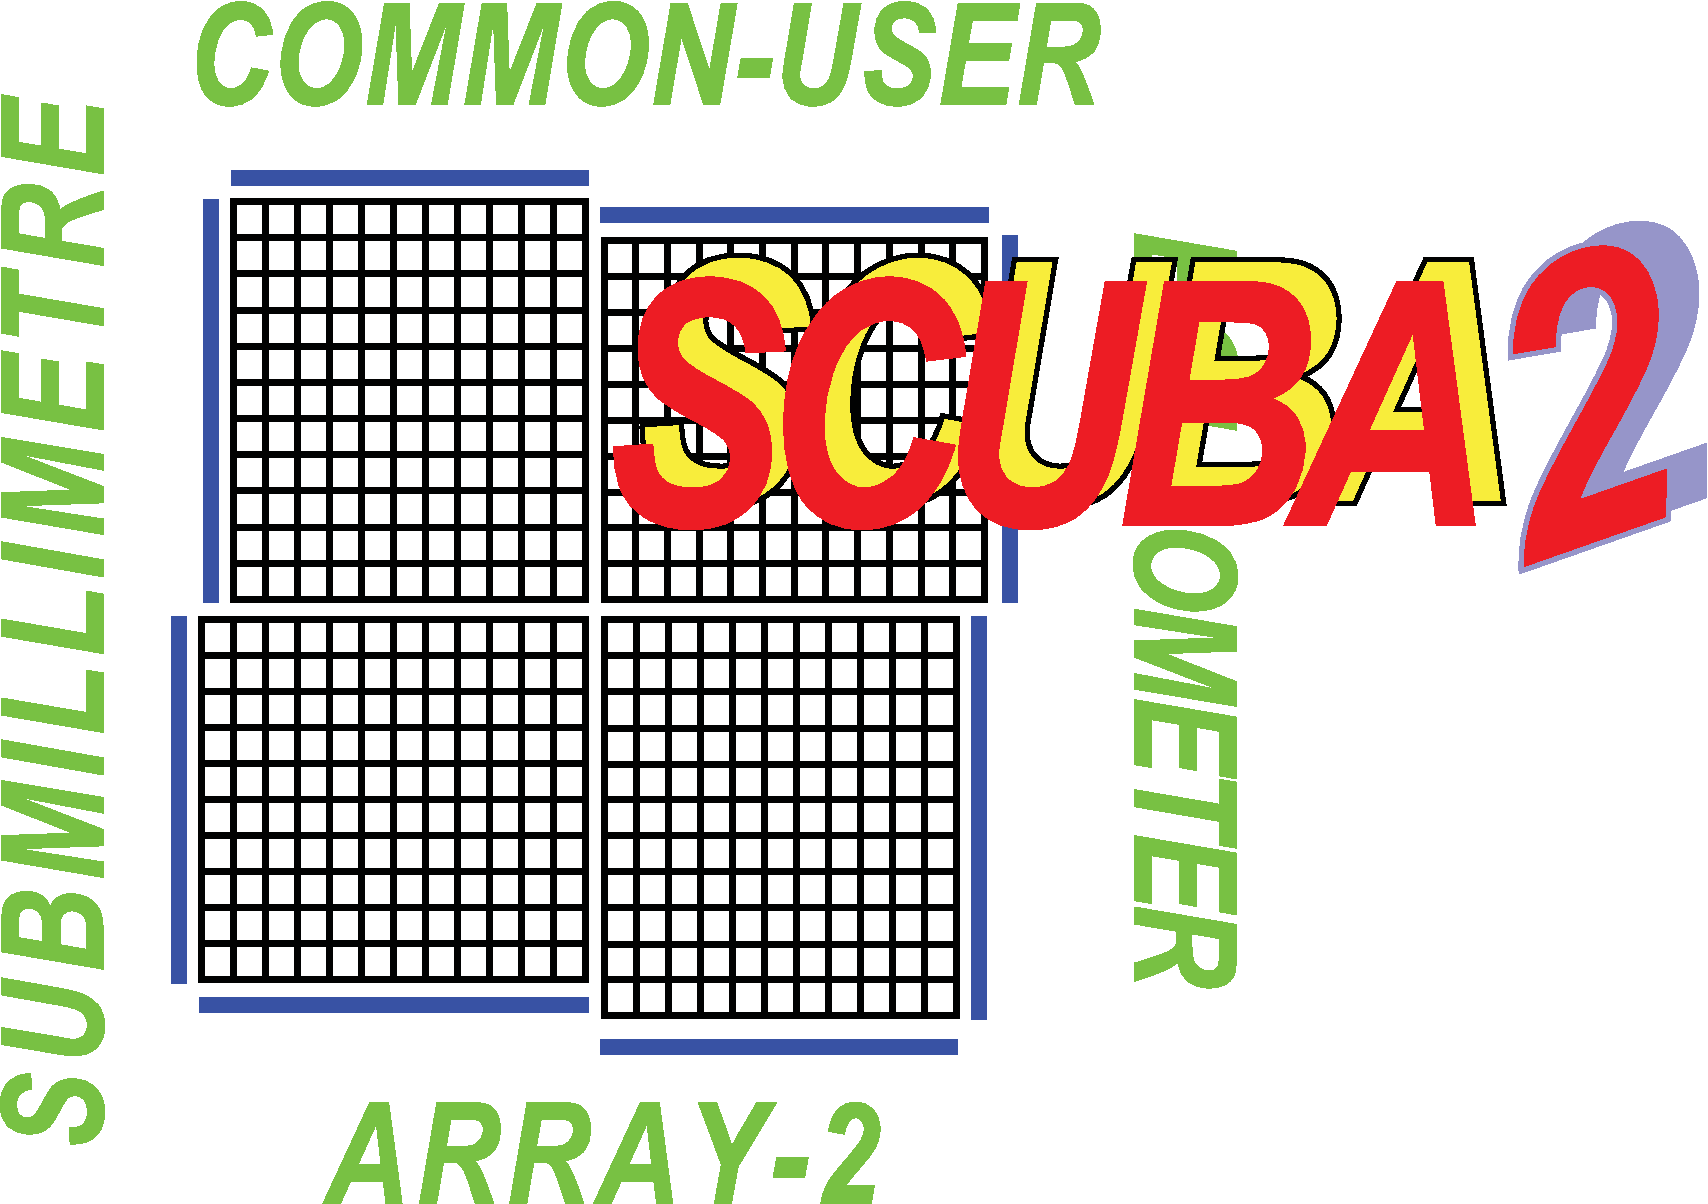
\includegraphics[scale=0.4]{sc21_s2logo}
   \end{center}
   \vspace{5mm}
   \rule{\textwidth}{0.5mm}\\
   \vspace{15mm}

% ? Heading for abstract if used.
   \vspace{10mm}
   \begin{center}
      {\Large\textbf{Abstract}}
   \end{center}
% ? End of heading for abstract.
\end{latexonly}

%  HTML documentation header.
%  ==========================
\begin{htmlonly}
   \xlabel{}
   \begin{rawhtml} <H1> \end{rawhtml}
      \stardoctitle\\
      \stardocversion\\
      \stardocmanual
   \begin{rawhtml} </H1> <HR> \end{rawhtml}

% ? Add picture here if required for the hypertext version.
%   e.g. \includegraphics[scale=0.5]{filename.ps}
   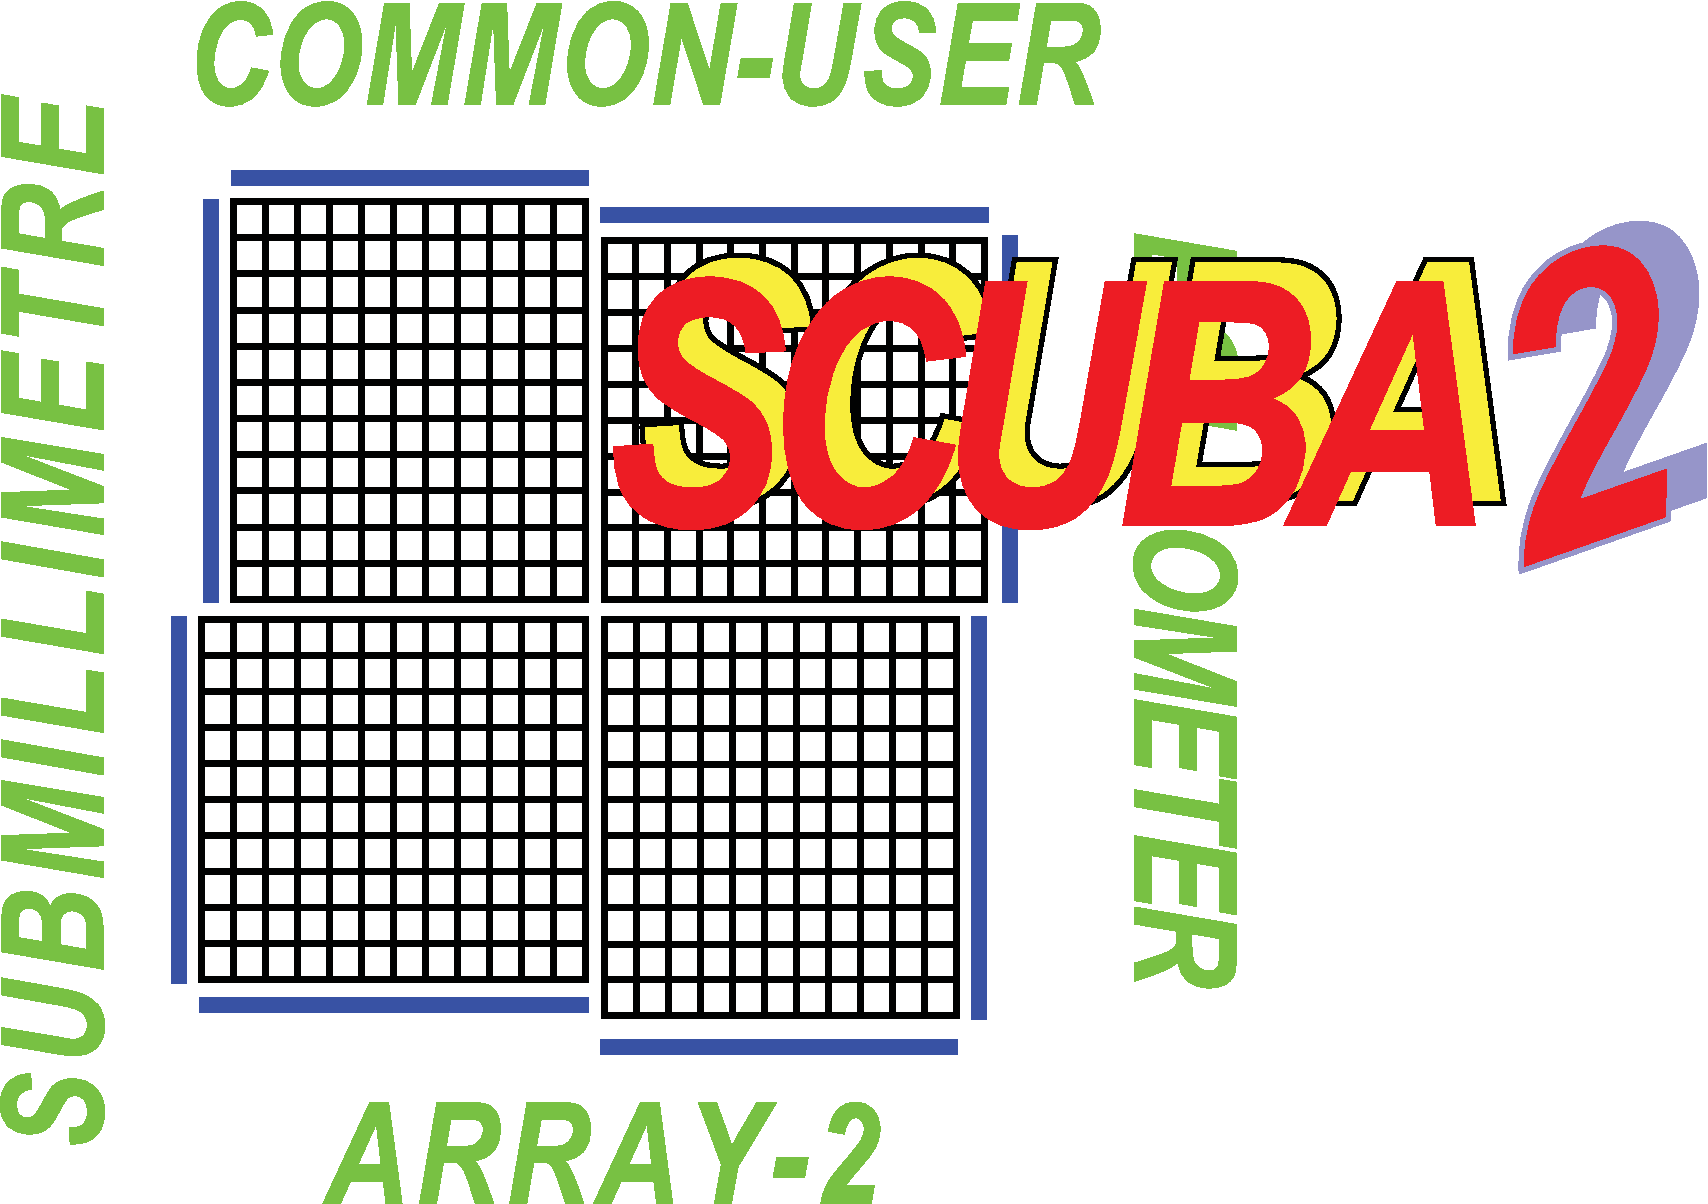
\includegraphics[width=90mm]{sc21_s2logo}
% ? End of picture

   \begin{rawhtml} <P> <I> \end{rawhtml}
   \stardoccategory\ \stardocnumber \\
   \stardocauthors \\
   \stardocdate
   \begin{rawhtml} </I> </P> <H3> \end{rawhtml}
      \htmladdnormallink{Joint Astronomy Centre}
                        {http://www.jach.hawaii.edu}\\
      \htmladdnormallink{Science \& Technology Facilities Council}
                        {http://www.scitech.ac.uk} \\
   \begin{rawhtml} </H3> <H2> \end{rawhtml}
      \htmladdnormallink{Starlink Project}{http://www.starlink.ac.uk/}
   \begin{rawhtml} </H2> \end{rawhtml}
   \htmladdnormallink{\htmladdimg{source.gif} Retrieve hardcopy}
      {http://www.starlink.ac.uk/cgi-bin/hcserver?\stardocsource}\\

%  HTML document table of contents.
%  ================================
%  Add table of contents header and a navigation button to return to this
%  point in the document (this should always go before the abstract \section).
  \label{stardoccontents}
  \begin{rawhtml}
    <HR>
    <H2>Contents</H2>
  \end{rawhtml}
  \htmladdtonavigation{\htmlref{\htmladdimg{contents_motif.gif}}
        {stardoccontents}}

% ? New section for abstract if used.
  \section{\xlabel{abstract}Abstract}
% ? End of new section for abstract
\end{htmlonly}

% -----------------------------------------------------------------------------
% ? Document Abstract. (if used)
%  ==================
\stardocabstract
% ? End of document abstract

% -----------------------------------------------------------------------------
% ? Latex Copyright Statement
%  =========================
\begin{latexonly}
\newpage
\vspace*{\fill}
\stardoccopyright
\end{latexonly}
% ? End of Latex copyright statement

% -----------------------------------------------------------------------------
% ? Latex document Table of Contents (if used).
%  ===========================================
  \newpage
  \begin{latexonly}
    \setlength{\parskip}{0mm}
    \tableofcontents
    \setlength{\parskip}{\medskipamount}
    \markboth{\stardocname}{\stardocname}
  \end{latexonly}
% ? End of Latex document table of contents
% -----------------------------------------------------------------------------

\cleardoublepage
\renewcommand{\thepage}{\arabic{page}}
\setcounter{page}{1}

\section{\xlabel{introduction}Introduction}
\label{sec:intro}

\subsection{\xlabel{using_guide}This Cookbook}

The Submillimetre Common User Bolometer Array-2 (SCUBA-2) is a
10,000-pixel bolometer camera for the 15-m James Clerk Maxwell
Telescope (JCMT). It has two arrays operating simultaneously to map
the sky in the atmospheric windows of 450 and 850$\mu$m.

This guide is designed to instruct SCUBA-2 users on the best ways to
reduce and visualise their data using \starlink\ packages,
\smurf\ \cite{smurf}, \Kappa\ \cite{kappa}, \gaia\ \cite{gaia}, \oracdr\ \cite{oracdr} and \picard\
\cite{picard}. This guide is {\em not} aimed at users of the
polarimeter (POL-2) or Fourier transform spectrometer (FTS-2). If you
have shared risk data (SRO) you should refer to the
\xref{SMURF SRO
Cookbook.}{sc19}{}\latex{\footnote{\texttt{http://www.starlink.ac.uk/docs/sc19.htx/sc19.html}}}

A brief description of the instrument and the observing modes is given
in \cref{Section}{sec:s2}{an Overview}. Details on data acquisition and
instructions for examining raw data are given in
\cref{Section}{sec:raw}{Raw SCUBA-2 data}.
\cref{Section}{sec:dimm}{This page} introduces the Dynamic Iterative Map-Maker
(DIMM); it offers an in-depth description of the map-making
process and introduces the configuration files necessary to run the
reduction. \cref{Section}{sec:maps}{Reducing your Data} covers running
the map-maker and what to look out for, while
\cref{Section}{sec:postprocess}{Post-processing Reduction Steps}
outlines the main post-processing steps you may wish to apply to your
science map, this includes applying the flux conversion
factor (FCF), coadding multiple maps and estimating the noise.
\cref{Section}{sec:tweak}{Tweaking the configuration file}
discusses your options for adjusting the configuration
parameters when running the map-maker; this gives you added control
and flexibility over the map-making routine. Two worked examples
covering different science case are shown in
\cref{Section}{sec:eg}{Examples}---a
\htmlref{blank cosmology field}{sec:cosmology}
\begin{latexonly}
(\S\ref{sec:cosmology})
\end{latexonly}
and a \htmlref{galactic field}{sec:bright_ex}
\begin{latexonly}
(\S\ref{sec:bright_ex})
\end{latexonly}
with bright, extended emission.
\cref{Section}{sec:pipe}{SCUBA-2 Pipeline} introduces the science
pipeline and data retrieval from the
\htmladdnormallink{JCMT Science Archive}{http://www3.cadc-ccda.hia-iha.nrc-cnrc.gc.ca/jcmt/}


\subsection{\xlabel{computing}Before you start: Computing resources}

Before reducing SCUBA-2 data using the Dynamic Iterative Map-Maker, we
recommend you confirm your resources are sufficient for your type of
map.

For large-area maps it is important to process a full observation in a
single chunk---see the text box on
\latexhtml{Page~\pageref{page:text}}{\htmlref{What to look
for}{box:chunk}} for a
discussion of the effects of chunking. For normal map-maker parameters
this implies that a machine of 96\,GB should be acceptable. It is
important that the memory is as fast as can be afforded as RAM speed
has a direct linear effect on processing time given that the
time-series data are continually being funneled through the CPU. For
blank field surveys, data that only use 850 microns, or smaller
regions of the sky you can usefully run the map-maker with less memory
and 32 to 64\,GB is reasonable depending on the specifics of your data
set. SMURF is multi-threaded so multiple cores do help although above
8 cores the price/performance gains tend to drop off.

If you have a very large machine (128\,GB and 24 cores) you can to run
two instances of the map-maker in parallel. Use the SMURF\_THREADS
environment variable to restrict each map-maker to half the available
cores.


\subsection{\xlabel{software}Before you start: Software}

This manual utilises software from the \starlink\ package;
\smurf\ \cite{smurf}, \Kappa\ \cite{kappa}, \gaia\ \cite{gaia}, \oracdr\ \cite{oracdr} and
\picard\ \cite{picard}. Starlink software must be installed on your system, and Starlink aliases
and environment variables must be defined before attempting any
reduction of SCUBA-2 data detailed here.

The Sub-Millimetre User Reduction Facility, or \textsc{Smurf}, contains the
Dynamic Iterative Map-Maker (DIMM) that will process raw SCUBA-2 data
into images (see \smurfsun). \textsc{Kappa} meanwhile is an application
package comprising general purpose commands for manipulating and
visualising NDF data (see \kappasun). Before starting any data
reduction you will want to initiate both \textsc{Smurf} and \textsc{Kappa}.
\begin{myquote}
\begin{verbatim}
% smurf

        SMURF commands are now available -- (Version 1.5.0)

        Type smurfhelp for help on SMURF commands.
        Type 'showme sun258' to browse the hypertext documentation.
        Type 'showme sc21' to view the SCUBA-2 map-making cookbook.

% kappa

     KAPPA commands are now available -- (Version 2.0-9)

     Type kaphelp for help on KAPPA commands.
     Type 'showme sun95' to browse the hypertext documentation.

     See the 'Release Notes' section of SUN/95 for details of the
     changes made for this release.
\end{verbatim}
\end{myquote}
Image visualisation can be done with \gaia\ (see \gaiasun). \gaia\ is an
image and data-cube display and analysis tool which incorporates tools such
as source detection, 3\textsc{d} visualisation, photometry and the ability
to query and overlay on-line or local catalogues.
\begin{myquote}
\begin{verbatim}
% gaia 850_map.sdf
\end{verbatim}
\end{myquote}

The \oracdr\ Data Reduction Pipeline \cite{oracdr} (hereafter just
\textsc{Orac-dr}) is an automated reduction pipeline. \textsc{Orac-dr} uses
\smurf\ and \Kappa\ (along with other Starlink tools) to perform an automated
reduction of the raw data following pre-defined recipes to produce
calibrated maps. \textsc{Picard} uses a similar pipeline system for
post-processing analysis of reduced data. \textsc{Picard}
documentation can be found at \htmladdnormallinkfoot{the \textsc{Orac-dr} web
page}{http://www.oracdr.org/oracdr/PICARD}, or at \picardsun. All
\textsc{Picard} recipes follow the same structure and are run like so:
\begin{myquote}
\begin{verbatim}
% picard -recpars <recipe_params_file> RECIPE <input_files>
\end{verbatim}
\end{myquote}
where \param{<recipe\_param\_file>} is a text file containing the
relevant recipe parameters, \param{RECIPE} is the name of the recipe
to be run (note the caps) and \param{<input\_files>} is a list of
files to be run, which must be int the current directory, or a
directory defined by \param{ORAC\_DATA\_OUT}. A number of \textsc{Picard}
recipes will be demonstrated in \cref{Section}{sec:maps}{Reducing your data}.

\textbf{Note:} The \textsc{Picard} recipes require all input files to have
the \texttt{.sdf} extension included; this is not the case for the
Starlink packages \textsc{Kappa} and \textsc{Smurf}.

\subsection{\xlabel{options}Processing Options}

There are two approaches to processing your data: either performing
each step by hand or by using an automated pipeline. The pipeline
approach works well if your project is suited to using one of the
standard recipes, and if you have a lot of data to process. Performing
each step by hand allows more fine-grained control of certain
processing and analysis steps, and is especially useful for refining
the parameters used by the map-maker. Of course, once the optimal
parameters have been determined, it is possible to pass them to the
pipeline and let it process all of your data automatically. Sections~4
and 5 discuss the manual approach; to use the science pipeline, skip
straight to \cref{Section}{sec:pipe}{SCUBA-2 Pipeline}.

While you have the option of running the pipeline yourself, the JCMT
will also produce pipeline reduced files for each observation and
group of repeat observations for each night. These are reduced using
the \oracdr\ pipeline with the recipe specified in the MSB.
\cref{Section}{sec:pipe}{SCUBA-2 Pipeline} gives instruction on
retrieving reduced data from the
\htmladdnormallink{JCMT Science Archive}{http://www3.cadc-ccda.hia-iha.nrc-cnrc.gc.ca/jcmt/}
at CADC.


\clearpage
\section{\xlabel{scuba2_overview}SCUBA-2 Overview}
\subsection{\xlabel{scuba2}The instrument}
\label{sec:s2}

The SCUBA-2 bolometers are integrated arrays of superconducting
transition edge sensors (TESs) with a characteristic transition
temperature, $T_c$. In addition, each TES is ringed with a resistive
heater which can compensate for changes in sky power. The SCUBA-2
focal plane is kept at a base temperature slightly below $T_c$,
however a voltage is applied across each TES resistance to position
the bolometer at the transition temperature. From this point, any
increase of temperature on the bolometers (e.g. from an astronomical
signal) will increase the TES resistance and heat it up. This causes a
drop in current and therefore a drop in temperature making the system
self-regulating.

For properly performing bolometers, the change in current through the
TES is proportional to the change in resistance, with the response
calibrated using flat-field observations (described below). This
changing current generates a magnetic field which is amplified by a
chain of superconducting quantum interference devices (SQUIDs). This
induces a feedback current which is proportional to the current
flowing through the TES, and it is this feedback current that is
recorded during data acquisition.

Before science data can be taken the system must be optimised. These
`setups' are performed after slewing to the azimuth of the source,
where the SQUID, TES and heater biases are set to pre-determined
nominal values, in order to position the bolometers in the middle of
the transition range.

This is followed by a 10-second noise observation carried out while
the shutter is still closed. The shutter then opens onto the sky, and
as it does so the gradual increase in sky power hitting the array is
compensated for by a decrease in the resistive heater power via a
servo loop designed to keep the TES output constant. This acts to keep
the bolometers positioned at the centre of the transition range and is
known as \textbf{heater tracking}.

The responsivity of the bolometers will change slightly between the
dark and the sky; therefore, once the shutter is fully open a fast
\textbf{flat-field} observation is carried out to recalibrate them.
\textbf{A flat-field measures the responsivity of each bolometer to
changing sky power}. It does this by utilising the resistance heaters
which are ramped up and down around the nominal value. The change in
current through the TES is then recorded for each bolometer giving a
measure of its responsivity. The flat field solution is then the
inverse linear gradient of the current as a function of heater power.

At this point bolometers with responsivities above or below a
threshold limit are rejected, along with bolometers which display a
non-linear response or have a poor SNR. A second flat-field is
performed at the end of an observation so bolometers whose
responsivity has changed over the course of the observation can be
flagged.

For full details of the array setup and operation see Holland et al.
(2013) \cite{s2main}.

\begin{figure}[t!]
\begin{center}
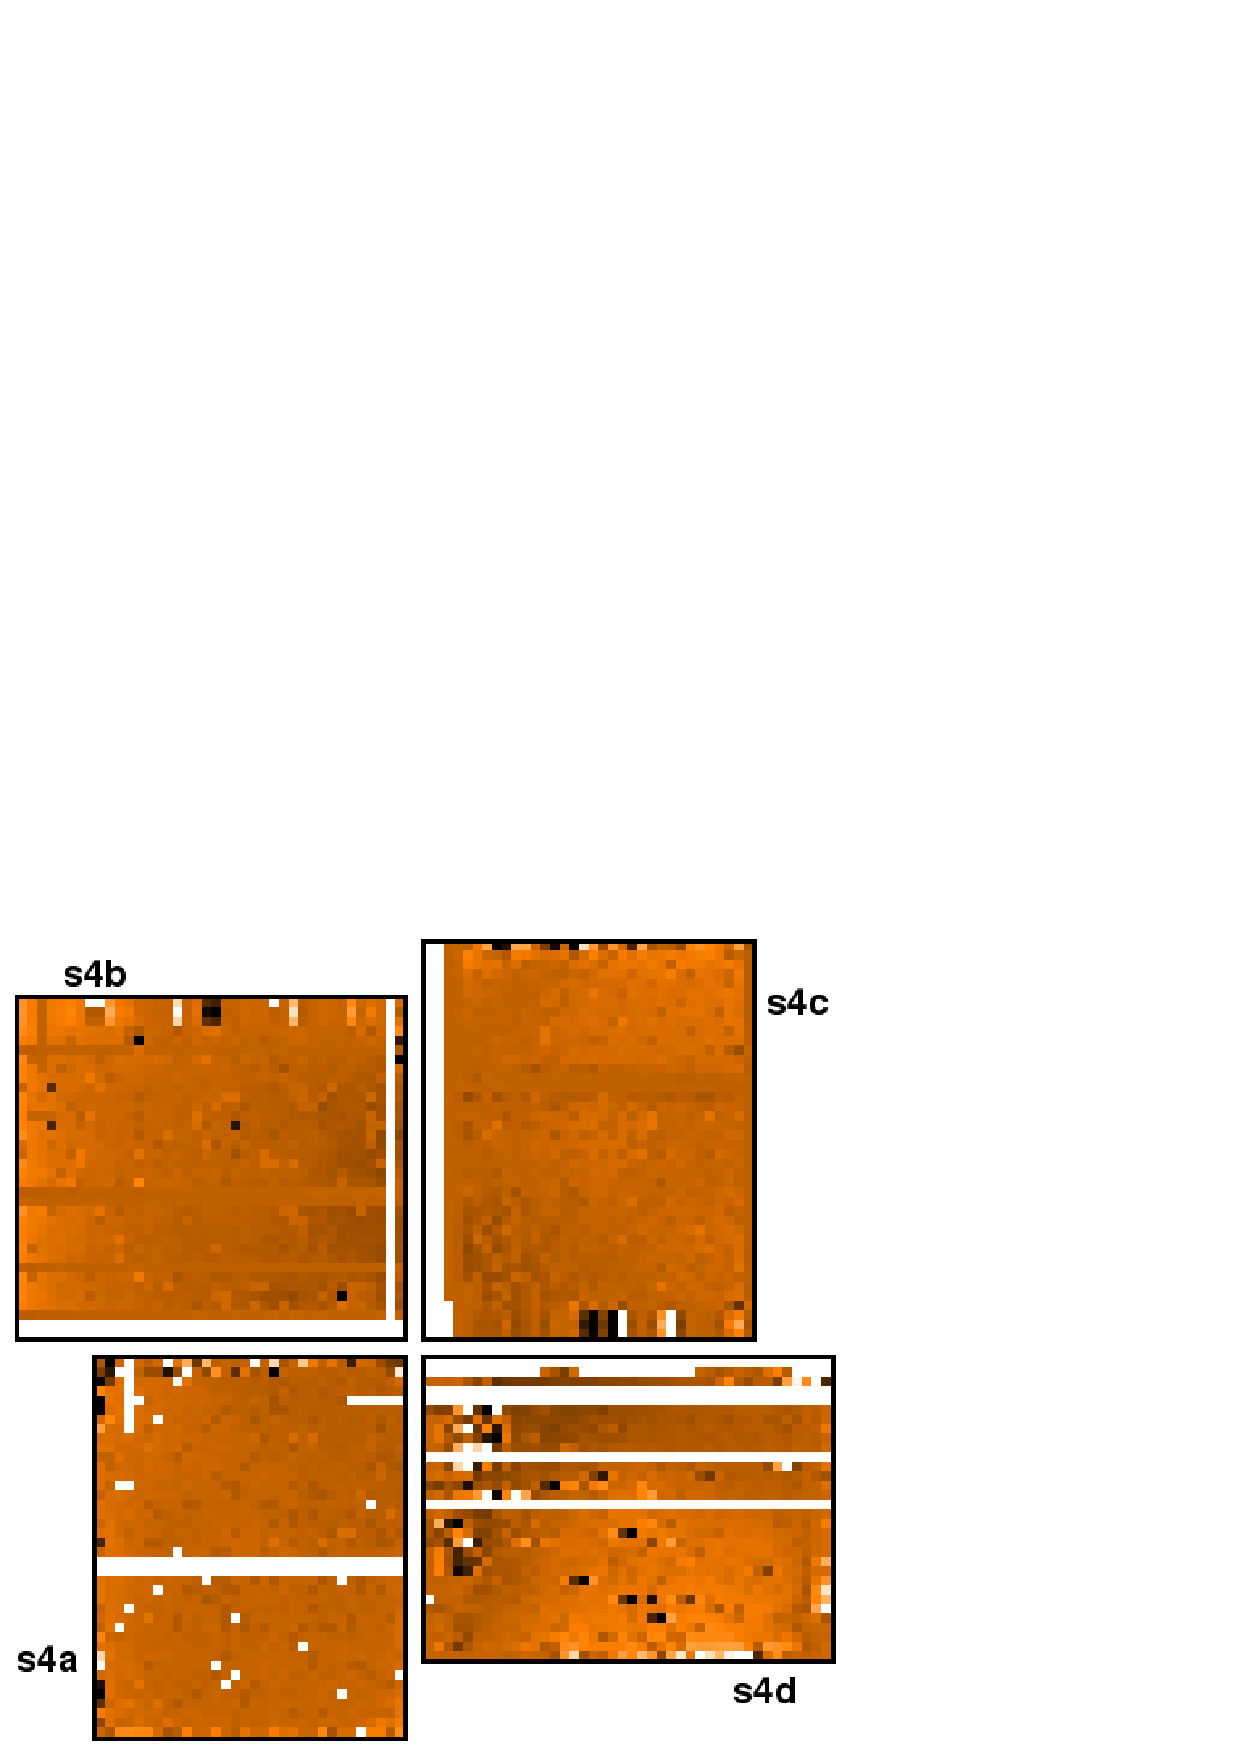
\includegraphics[width=0.4\linewidth]{sc21_450array}
\hspace{1cm}
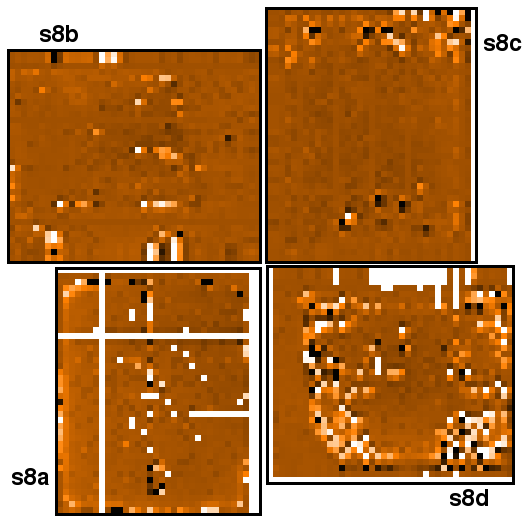
\includegraphics[width=0.4\linewidth]{sc21_850array}
\label{fig:arrays}
\caption{\small The layout of the arrays at 450$\mu$m (left) and
850$\mu$m (right). The labels denote the name assigned to each
sub-array. Raw data files are generated separately for each sub-array
and must be coadded. This figure was made my running \wcsmosaic\ on
raw files from each sub-array.}
\end{center}
\end{figure}

\subsection{\xlabel{obs_modes}Observing modes}
\label{sec:mmodes}

Two observing modes are offered for SCUBA-2---\textsc{daisy} and
\textsc{pong}. As much of the work SCUBA-2 will be doing involves
large area mapping, both observing modes are scan patterns. Your
choice depends on the size of the area you wish to map, where you
would like your integration time concentrated and the degree of
extended emission you wish to recover

In contrast to SCUBA which observed an area of sky while
simultaneously chopping, SCUBA-2 removes atmospheric noise in the data
processing stage (Holland et al. 2013) \cite{s2main}. The power spectrum
of data taken by SCUBA-2 has a $1/f$ noise curve at lower frequencies. To
ensure astronomical signals are far away from this $1/f$ noise, fast
scanning speeds are required.

In order to disentangle source structure from other
slowly varying signals (e.g. extinction, sky noise, $1/f$ noise), the
scan pattern must pass across each region of the map from different
directions and at different times. The scan patterns themselves, along
with the associated parameters (velocity and scan-spacing), have been
designed and optimised to meet both these criteria.
\\ \\
\begin{minipage}[t]{0.12\linewidth}
\textbf{PONG}
\end{minipage}
\begin{minipage}[t]{0.85\linewidth}\textsc{pong} maps are the scan
strategy for covering large areas. The default options allow for 3
sizes---900\,arcsec, 1800\,arcsec and 3600\,arcsec. A single \textsc{pong} map is
a square of these dimensions and the telescope fills in the square by
bouncing off the edge of the area. To ensure an even sky background it
is recommended a minimum of 3, but preferably more than 5,
\textsc{pong} maps are included in a single observation with a
rotation introduced between each one. In this way a circular pattern
is built up, (see the right-hand panel of \cref{Figure}{fig:scan}{graphic below}),
with a diameter equal to your requested map size.
\vspace{0.2cm}\\
To recover large-scale extended structure you are advised to use
larger \textsc{pong} maps which scan at a higher rate. This option is
in preference to tiling multiple smaller maps.
\end{minipage}
\\ \\ \\
\begin{minipage}[t]{0.12\linewidth}
\textbf{DAISY}
\end{minipage}
\begin{minipage}[t]{0.85\linewidth}
\textsc{daisy} maps are the option for point-like or compact sources
($<$3~arcmin) by maximising the exposure time on the centre of the
image. The telescope moves at a constant velocity in a `spirograph'
pattern that has the advantage of keeping the source on the array
throughout the observation. This is shown in the top panel of
\cref{Figure}{fig:scan}{the figure below}.
\end{minipage}

\myfig{sc21_wayne_scan}{[b!]}{width=0.9\linewidth}{fig:scan}{
  Telescope track in offsets of azimuth and elevation for the SCUBA-2
  observing patterns. \textbf{Top Left}: A single rotation of the
  \textsc{daisy} pattern; \textbf{Top Right}: Multiple rotations of
  the \textsc{daisy} pattern for a typical map based on a 180-arcsec
  demanded diameter; \textbf{Bottom Left}: A single \textsc{pong}
  pattern; \textbf{Bottom Right}: Multiple rotations of the
  \textsc{pong} pattern for a typical map based on an 1800-arcsec
  demanded map size. The scan pattern for your observation can be
  visualised like this with \topcat\ using the output from \jcmtstate.
  See \cref{Section}{sec:exam}{Examining raw data} for more details.
  Figure taken from Holland et al. (2013).}

\clearpage

\section{\xlabel{data_files}Raw SCUBA-2 Data}
\label{sec:raw}

A normal science observation will follow the following sequence.
\vspace{-2mm}
\begin{itemize}\itemsep-0.5em
\item Noise
\item Flat-field
\item Multiple Science scans
\item Flat-field
\end{itemize}
\vspace{-2mm}
The \param{SEQ\_TYPE} parameter in the FITS header may be used to
identify the nature of each scan (see
\cref{Section}{sec:fitsheader}{Headers and file structure}).
When you access you data either at the JCMT or by downloading from the
\htmladdnormallink{Science Archive}{http://www3.cadc-ccda.hia-iha.nrc-cnrc.gc.ca/jcmt/}
\begin{latexonly}
\footnote{\texttt{http://www3.cadc-ccda.hia-iha.nrc-cnrc.gc.ca/jcmt/}}
\end{latexonly}
you will get \emph{all} of the files listed above. Later when you
reduce your data using the map-maker you will include \emph{all} of
the files (noise + flat-fields + science).
Shown below is a list of the raw files for a single sub-array (in this
case s8a) for a short calibration observation. The first file is a
short, dark noise; the second and last scans are fast flat-field
observations which occur after the shutter opens to the sky at the
start of the observation and closes at the end (note the identical
file size); all of the scans in between are science. The SCUBA-2 data
acquisition (DA) system writes out a data file every 30 seconds; each
of which contains 23\,MB of data. The only exception is the final science
scan which will usually be smaller (7.3\,MB in the example below), typically
requiring less than 30 seconds of data to complete the observation.
\begin{myquote}
\begin{verbatim}
-rw-r--r-- 1 jcmtarch jcmt 6.2M Jul 19 21:33 s8a20120720_00030_0001.sdf
-rw-r--r-- 1 jcmtarch jcmt 9.6M Jul 19 21:34 s8a20120720_00030_0002.sdf
-rw-r--r-- 1 jcmtarch jcmt 23M Jul 19 21:34 s8a20120720_00030_0003.sdf
-rw-r--r-- 1 jcmtarch jcmt 23M Jul 19 21:35 s8a20120720_00030_0004.sdf
-rw-r--r-- 1 jcmtarch jcmt 23M Jul 19 21:36 s8a20120720_00030_0005.sdf
-rw-r--r-- 1 jcmtarch jcmt 23M Jul 19 21:36 s8a20120720_00030_0006.sdf
-rw-r--r-- 1 jcmtarch jcmt 7.3M Jul 19 21:36 s8a20120720_00030_0007.sdf
-rw-r--r-- 1 jcmtarch jcmt 9.6M Jul 19 21:37 s8a20120720_00030_0008.sdf
\end{verbatim}
\end{myquote}
\textbf{Note:} All of these files are written out 8 times for each of the
8 sub-arrays.

The main data arrays of each file are cubes, with the first two
dimensions enumerating columns and rows, and the third time slices
(sampled at 200\,Hz).

Raw SCUBA-2 data are written as uncalibrated digitised data. The first calibration
step is to scale the raw data to units proportional to picowatts (pW)
by applying the flat-field solution. From there the data must be
scaled by the flux conversion factor (FCF) to give units of Janskys
(Jy).

The first step is applied internally by the map-maker but can be done
manually when examining the raw data---see
\cref{Section}{sec:concat}{Concatenate \& apply a flat-field}.
The second step must be done manually with the instructions given in
\cref{Section}{sec:cmult}{Applying the FCF and determining fluxes}.


\subsection{\xlabel{examine}Examining raw data}
\label{sec:exam}

In this section a number of procedures are described for visualising
and assessing raw data files. These steps are not a necessary part of
the data reduction process and do not concern the iterative map-maker.
However, there are reasons you may wish to examine your raw data in
greater depth. The most likely motivation is an unusual result from the
map-maker, this could be higher than anticipated noise, patterns in
the data or inconsistent noise across multiple tiles. This section
will help you get to the bottom of any issues concerning raw data.

\subsubsection{\xlabel{concat}Concatenate \& apply a flat-field}
\label{sec:concat}

Since SCUBA-2 data for a given sub-array are broken into multiple
30-second scans by the data acquisition (DA) system, it is useful to
concatenate the data into a single file. The \smurf\ task \concat\ can
be used for this operation. The example below combines all of the
files associated with observation 45 for the s8a array into a single
file called \texttt{s8a20120725\_00045\_con}.

\begin{myquote}
\begin{verbatim}
% sc2concat 's8a20120725_00045*.sdf' s8a20120725_00045_con
\end{verbatim}
\end{myquote}
\task{sc2concat} will automatically filter out any dark or flat-field
observations, so that the concatenated file contains only the science
data. Be careful when concatenating a very long observation since the
output file may be too large to reasonably handle. Fifteen minute
chunks (30 files) should be sufficient.

\task{sc2concat} applies the flat-field by default (although it can be
disabled using the `noflat' option on the command-line).

The flat-field can also be applied manually using the \flatfield\ command.

\begin{myquote}
\begin{verbatim}
% flatfield 's8a20120701_00045*.sdf' '*_flat'
\end{verbatim}
\end{myquote}
Here, the output will be a flat-fielded version of each science scan
in observation number 8; the file names will be the original input
names with \_flat appended to them.

As a rule of thumb, you should apply the flat-field to your data
before examining it. \textbf{You do not need to apply the flat-field
prior to reducing your data with the map-maker as it will be applied
internally.}


\subsubsection{\xlabel{header}Headers and file structure}
\label{sec:fitsheader}

There are two \Kappa\ tasks which are extremely useful for examining
your data: \fitslist\ and \ndftrace, which can be used to view the
FITS headers and dimensions of the data.
\\ \\
\begin{minipage}[t]{0.12\linewidth}
\textbf{fitslist}
\end{minipage}
\begin{minipage}[t]{0.85\linewidth}This lists the FITS header information
for any file (raw or reduced). This extensive list includes dates \& times,
source name, scan type, pattern and velocity, size of the map, exposure
time, start and end elevation, opacity and the temperature of the
instrument. An example is given below:
\begin{myquote}
\begin{verbatim}
% fitslist s8a20120720_00030_0003.sdf
\end{verbatim}
\end{myquote}
If you already know the name of the parameter you want to view you can
either pipe the \task{fitslist} output to grep or use the \fitsval\ command
instead, e.g. \texttt{\% fitsval file.sdf TAU225ST}.\\
\end{minipage}

\begin{minipage}[t]{0.12\linewidth}
\textbf{ndftrace}
\end{minipage}
\begin{minipage}[t]{0.85\linewidth}
\task{ndftrace} displays the attributes of the data structure. This will tell
you the units of the data, pixel bounds, dimensions and axis assignations.\\
\end{minipage}
\\ \\
Full details of these commands can be found in the \xref{\textsc{Kappa} manual}{sun95}{}.

\begin{latexonly}
\begin{figure}[ht!]
\begin{center}
\begin{fmpage}{0.95\linewidth}
\vspace{0.2cm}
\textbf{ Topcat Example}

\vspace{0.5cm}

\begin{minipage}[c]{0.6\linewidth}

\begin{myquote}
\begin{verbatim}
% topcat -f tst 20120720_30.tst
\end{verbatim}
\end{myquote}
\end{minipage}
\hspace{0.3cm}
\begin{minipage}[c]{0.32\linewidth}
Load the file into \topcat\ with this command.
\end{minipage}

\vspace{0.5cm}

\begin{minipage}[c]{0.6\linewidth}
\centering
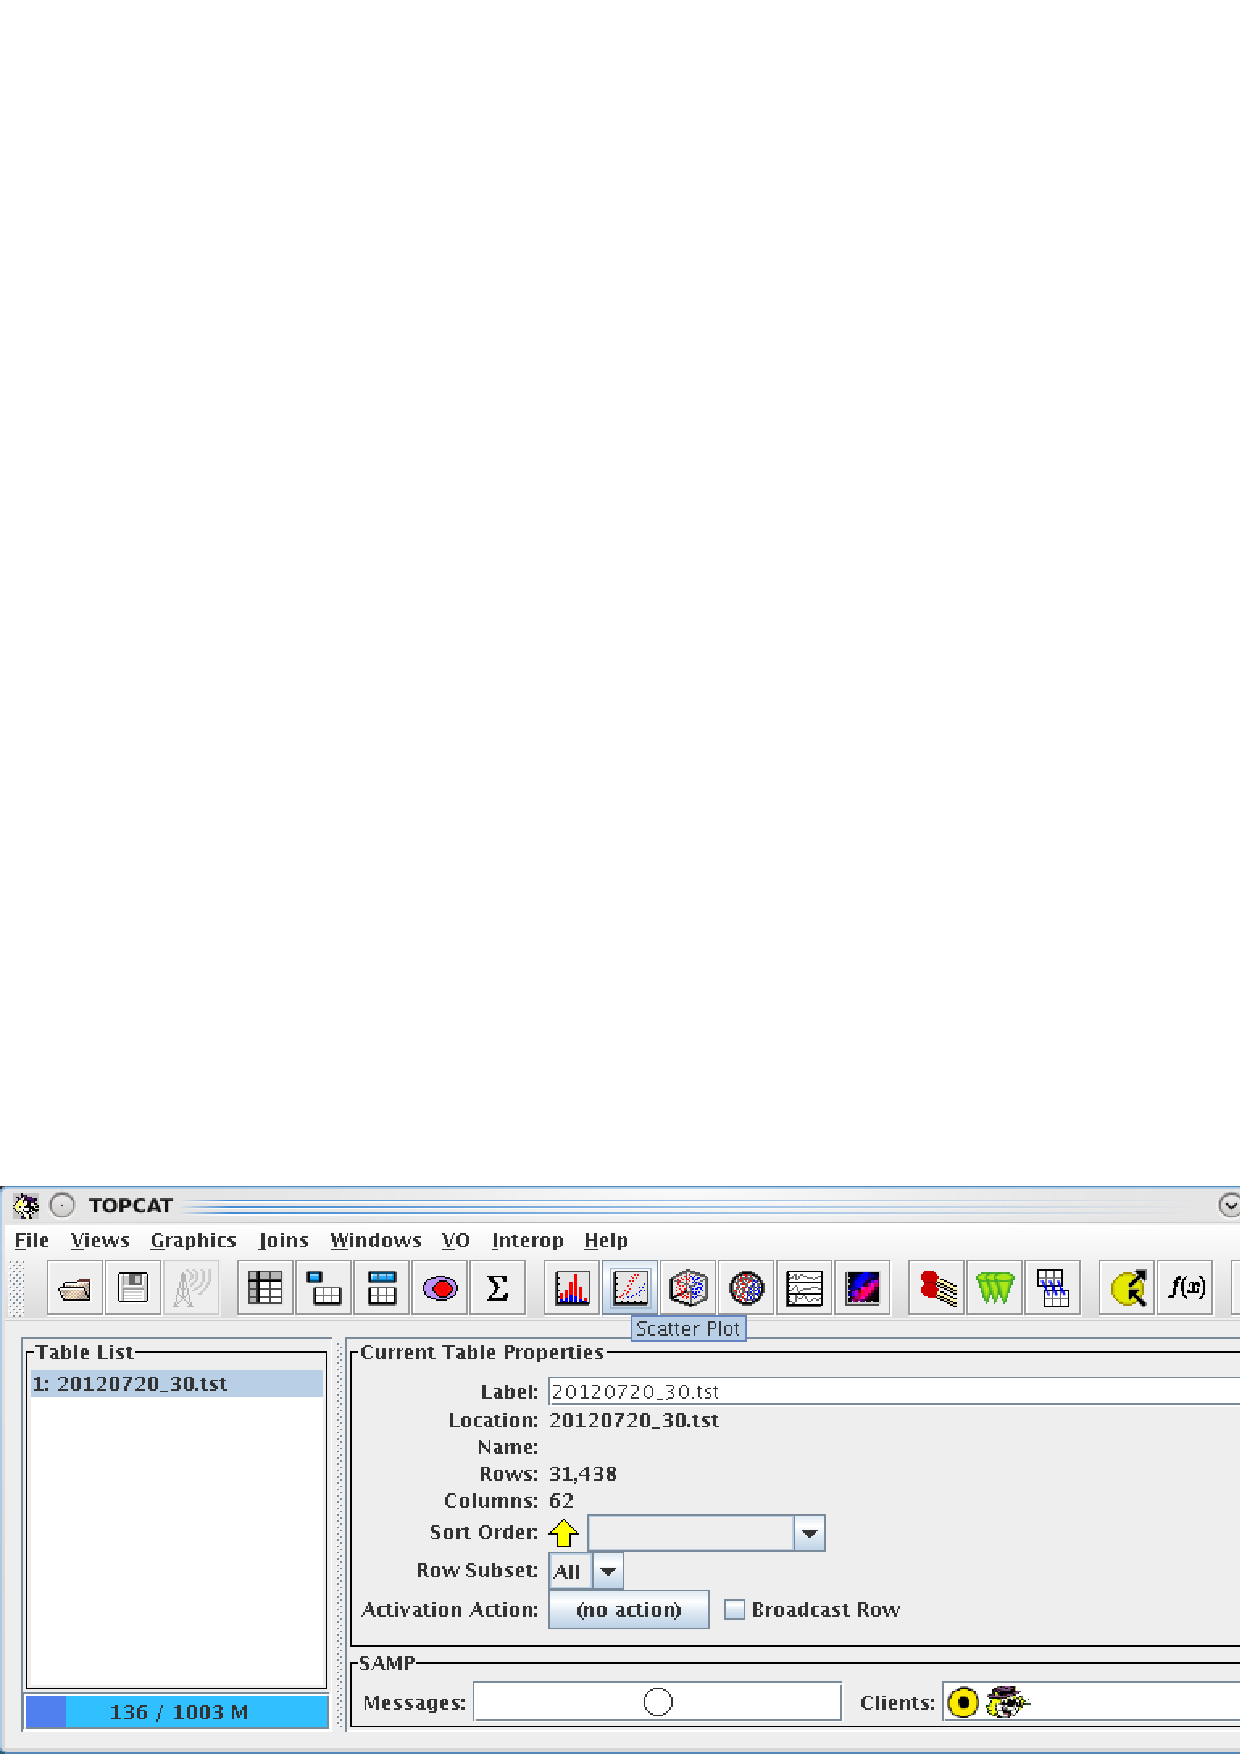
\includegraphics[width=0.95\textwidth]{sc21_topcat1}

\end{minipage}
\hspace{0.3cm}
\begin{minipage}[c]{0.32\linewidth}
Once the file has loaded into \topcat, select the scatter plot option
from the menu bar across the top of the window.
\end{minipage}

\vspace{0.5cm}

\begin{minipage}[c]{0.6\linewidth}
\centering
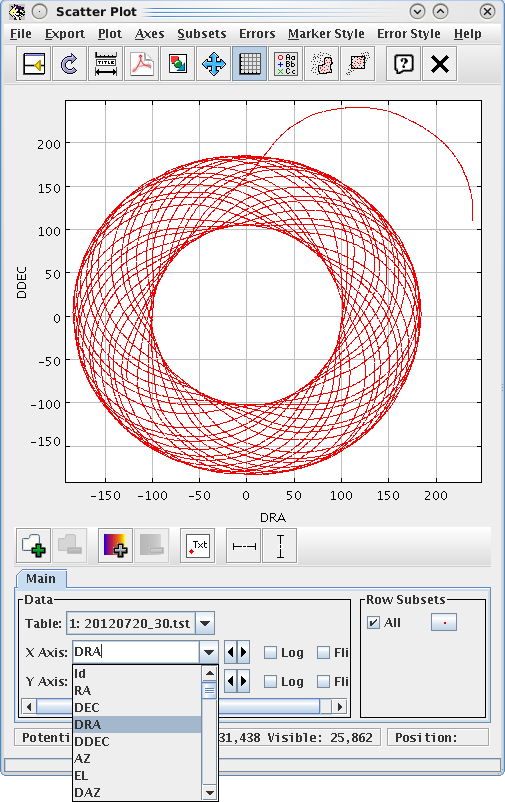
\includegraphics[width=0.75\textwidth]{sc21_topcat2}
\vspace{0.2cm}
\end{minipage}
\hspace{0.3cm}
\begin{minipage}[c]{0.32\linewidth}
When the scatter plot has loaded, you should adjust the $X$-axis and
$Y$-axis values to DRA and DDEC respectively to display the scan pattern.
If you are interested in seeing how any of the variables change over time,
select the the $X$ Axis to be either Id or RTS\_NUM.
\end{minipage}

\end{fmpage}
\end{center}
\caption{\small \topcat\ example demonstrating how to display the scan pattern
for an observation.}
\label{fig:topcat}
\end{figure}
\end{latexonly}


\subsubsection{\xlabel{scan_pat}Displaying scan patterns}
\label{sec:scan}

The movement of the telescope throughout a scan (as well as other
state information) is stored in the \texttt{MORE.SMURF.JCMTSTATE}
extension of a data file. The \smurf\ task \jcmtstate\ converts this
information into a simple ASCII tab-separated table.

\begin{myquote}
\begin{verbatim}
% jcmtstate2cat s8a20120701_00008_*.sdf > state.tst
\end{verbatim}
\end{myquote}

The \texttt{-h} option to \task{jcmtstate} can be used to find more
information on the command. In particular, multiple files can be supplied
to the command using standard shell wild cards. If you have already
concatenated your data you can simply input the single concatenated
file. \textbf{It may be useful to view the scan pattern for your
observation, particularly for maps taken at high elevations, to ensure
the pattern completed successfully.}

This catalogue can be loaded into \topcat\ for plotting, making sure
to specify the TST format during loading.

\begin{myquote}
\begin{verbatim}
% topcat -f tst state.tst
\end{verbatim}
\end{myquote}

Example of scan patterns displayed with \topcat\ can be seen in
\cref{Figure}{fig:scan}{telescope tracks}. Detailed instructions on
how to display the scan pattern for your observation are given in
\cref{Figure}{fig:topcat}{box below}.
All of the time-varying header values are available for plotting. Other
values include the azimuth and elevation offsets (DAZ \& DEL), the WVM
and 225\,GHz opacity values, and the instrument temperatures (e.g.
SC2\_FPUTEMP gives the temperature of the focal plane).

% The minipages used for the dvi version give latex2html problems.
\begin{htmlonly}
 \label{fig:topcat} \htmladdimg{sc21_topcat_example.png}
 \\
 Figure: \topcat\ example demonstrating how to display the scan
 pattern for an observation.\\ \\
\end{htmlonly}

Due to extreme accelerations at ``turn-around'' points of a scan
pattern (especially for \textsc{pong}s), the telescope finds it hard
to follow the proscribed scan patterns at high elevations. To mitigate
this we try to avoid observing any sources above 70$^\circ$ elevation.
If the \fitslist\ parameters \param{ELSTART} and \param{ELEND}
indicate that your map was taken at high elevation you may consider
checking the success of the scan pattern. If you find your observation
has failed to follow the demanded scan pattern don't worry, the data is
likely to still be useful. This is especially true for \textsc{daisy}
maps where the high exposure-time central region is usually
unaffected.

\subsubsection{\xlabel{display_cube}Displaying time-series data}
\label{sec:gaiacube}

Use the \starlink\ application \textsc{Gaia} to visualise the bolometer time
series data (or indeed \emph{any} SCUBA-2 data file). This is
initiated simply typing \texttt{gaia} into a terminal.

\begin{myquote}
\begin{verbatim}
% gaia s8a20120725_00058_con.sdf
\end{verbatim}
\end{myquote}

Loading a file in \textsc{Gaia} produces two windows (see
\cref{Figure}{fig:gaia_main}{upper graphic}). The main window shows a map of bolometer
values at a given point in time. The time slice displayed may be
changed by scrolling through the time axis. This is done in the second
window entitled `Display image sections of a cube'. The `Index of
plane' slider towards the top of this window may be moved to display
different time slices in the main window.

\myfig{sc21_gaia1}{[h!]}{width=\linewidth}{fig:gaia_main}{
  Initial \gaia\ windows displayed upon loading a data cube.
  The main window in the left shows a map of bolometer values at a fixed
  sample in time. You may have to zoom in multiple times by clicking the
  `Z' icon. On the right-hand side, the `Display image sections of a cube'
  dialogue enables you to navigate the time axis.}

A third window will appear when you click on a bolometer---the
`Spectral plot'. This shows an automatically scaled plot of the raw
time stream of data for that given bolometer. It will be overridden
when you click on a different bolometer.

\myfig{sc21_gaia2}{[h!]}{width=0.8\linewidth}{fig:gaia_spec}{
  The \emph{Spectral Plot} window displaying its time-varying
  signal, appears automatically once a bolometer is clicked in the main window.
  The vertical red line indicates the time slice that is currently selected
  in the `Display image sections of a cube' dialogue---this can be dragged
  across the spectrum to scroll through the time-slices.}

A second way to scroll through the time axis is to click and drag the
vertical red bar on the `Spectral plot' window. As you do so, the array
shown in the main window will automatically update.

To highlight small variations between bolometers it is likely you will
need to change the auto cut and (depending on your preference) the
colour scheme---both are controlled by buttons on the sidebar.

See the \xref{\textsc{Gaia} manual}{sun214}{} for full
details.\latex{\footnote{\texttt{http://docs.jach.hawaii.edu/star/sun214.htx/sun214.html}}}

\clearpage
\subsection{\xlabel{regrid_map}Regridding data into a map}
\label{sec:regrid}

Any raw time-series data can be quickly regridded into sky frame
coordinates using the \smurf\ \makemap\ task in rebin mode. This
involves no processing of the data. The following command produces a
map from the raw concatenated data; unlike the iterative mode of
\task{makemap} described in the next chapter, no configuration file is
required.
\begin{myquote}
\begin{verbatim}
% makemap s8a20120725_00058_con.sdf crl2688_sky method=rebin
\end{verbatim}
\end{myquote}
The output map here is called \texttt{crl2688\_sky.sdf} and is shown
in \cref{Figure}{fig:regrid}{the figure below}.
The pixel scale is left at the default values of 2\,arcsec on a side at
450\,$\mu$m and 4\,arcsec at 850\,$\mu$m (although this can be changed
using the \texttt{pixsize=}$x$ option on the command-line, where $x$ is in
arcsec).

\myfig{sc21_crl2688_regrid}{[b!]}{width=0.65\linewidth}{fig:regrid}{
  The regridded map of CRL2688 with the s8a sub-array displayed with \gaia.}


\subsection{\xlabel{clean}Notes on cleaning your data}
\label{sec:clean}

Cleaning raw data is an essential first step towards making a quality
final map. The map-maker performs all of these cleaning steps during
the pre-processing stage. The commands for manually cleaning your data
are given in \cref{Appendix}{app:clean}{Cleaning the Raw Data}.

% Split to avoid paragraph break mid-sentence.
\begin{htmlonly}
You can also check out the \xref{SMURF SRO Cookbook}{sc19}{} which
goes into great depth on the data cleaning options.
\end{htmlonly}
\begin{latexonly}
You can also check out the SMURF SRO
Cookbook{\footnote{\texttt{http://www.starlink.ac.uk/docs/sc19.htx/sc19.html}}}
which goes into great depth on the data cleaning options.
\end{latexonly}


\subsection{\xlabel{calcnoise}Checking the array performance}
\label{sec:calcnoise}

The on-sky performance of the array can be assessed using the \smurf\
command \calcnoise. Rather than give an absolute measure, \task{calcnoise}
should be used as an indicator of array performance and stability.
\task{calcnoise} cleans the data then calculates the
white noise on the array (between 2 and 10\,Hz by default). If the
dark noise scans are given as input, this will track the array
sensitivity independent of sky conditions. If you provide the whole
observation (as in the example below) then the dark files will be
ignored and the on-sky performance of the array is calculated.

\begin{myquote}
\begin{verbatim}
% calcnoise s8a20110720_00030*.sdf s8a_noise method=! power=!
\end{verbatim}
\end{myquote}
It will prompt for a configuration file to describe the cleaning
steps---recommended is the supplied \texttt{dimmconfig\_calcnoise.lis}.
Two noise measurements are reported in the terminal: the
`Effective noise' and the `Effective NEP'.

An output file is created for each sub-array with the NEP map stored
in the \texttt{.MORE.SMURF.NEP} extension.

If you have a bright source in the field this will contaminate the
signal which in turn will lead to an overestimate of the noise. In
this case you should examine the \texttt{NOI} model from the map-maker
instead---see \cref{Section}{sec:models}{The Individual Models} for a
description and \cref{Section}{sec:export}{Exporting individual
models} for details on how to examine it.

\clearpage
\section{\xlabel{dimm}The Dynamic Iterative Map-Maker}
\label{sec:dimm}

The Dynamic Iterative Map-Maker (DIMM), hereafter just referred to as
the map-maker is the tool you will use to produce SCUBA-2 maps. It
performs all pre-processing steps to clean the data, followed by
iteratively solving for multiple signal components and regridding to
produce a final science map.

This section describes the process by which the map-maker reduces
data. It is essential reading to gain an understanding of what has
happened to produce your reduced image, especially if you wish to
modify the default map-maker parameters. Nevertheless, this manual
is intended to present `need to know' information for data reduction.
For full details of the map-maker see Chapin et al. (2013) \cite{mapmaker}.

% Separated to make figure appear in a reasonable place in the
% PostScript.  Note using myfig command as originally coded causes
% "wrap_cmd_ not defined, cannot wrap \@" and similar errors in the l2h
% stage.
\begin{latexonly}
\begin{figure}
\centering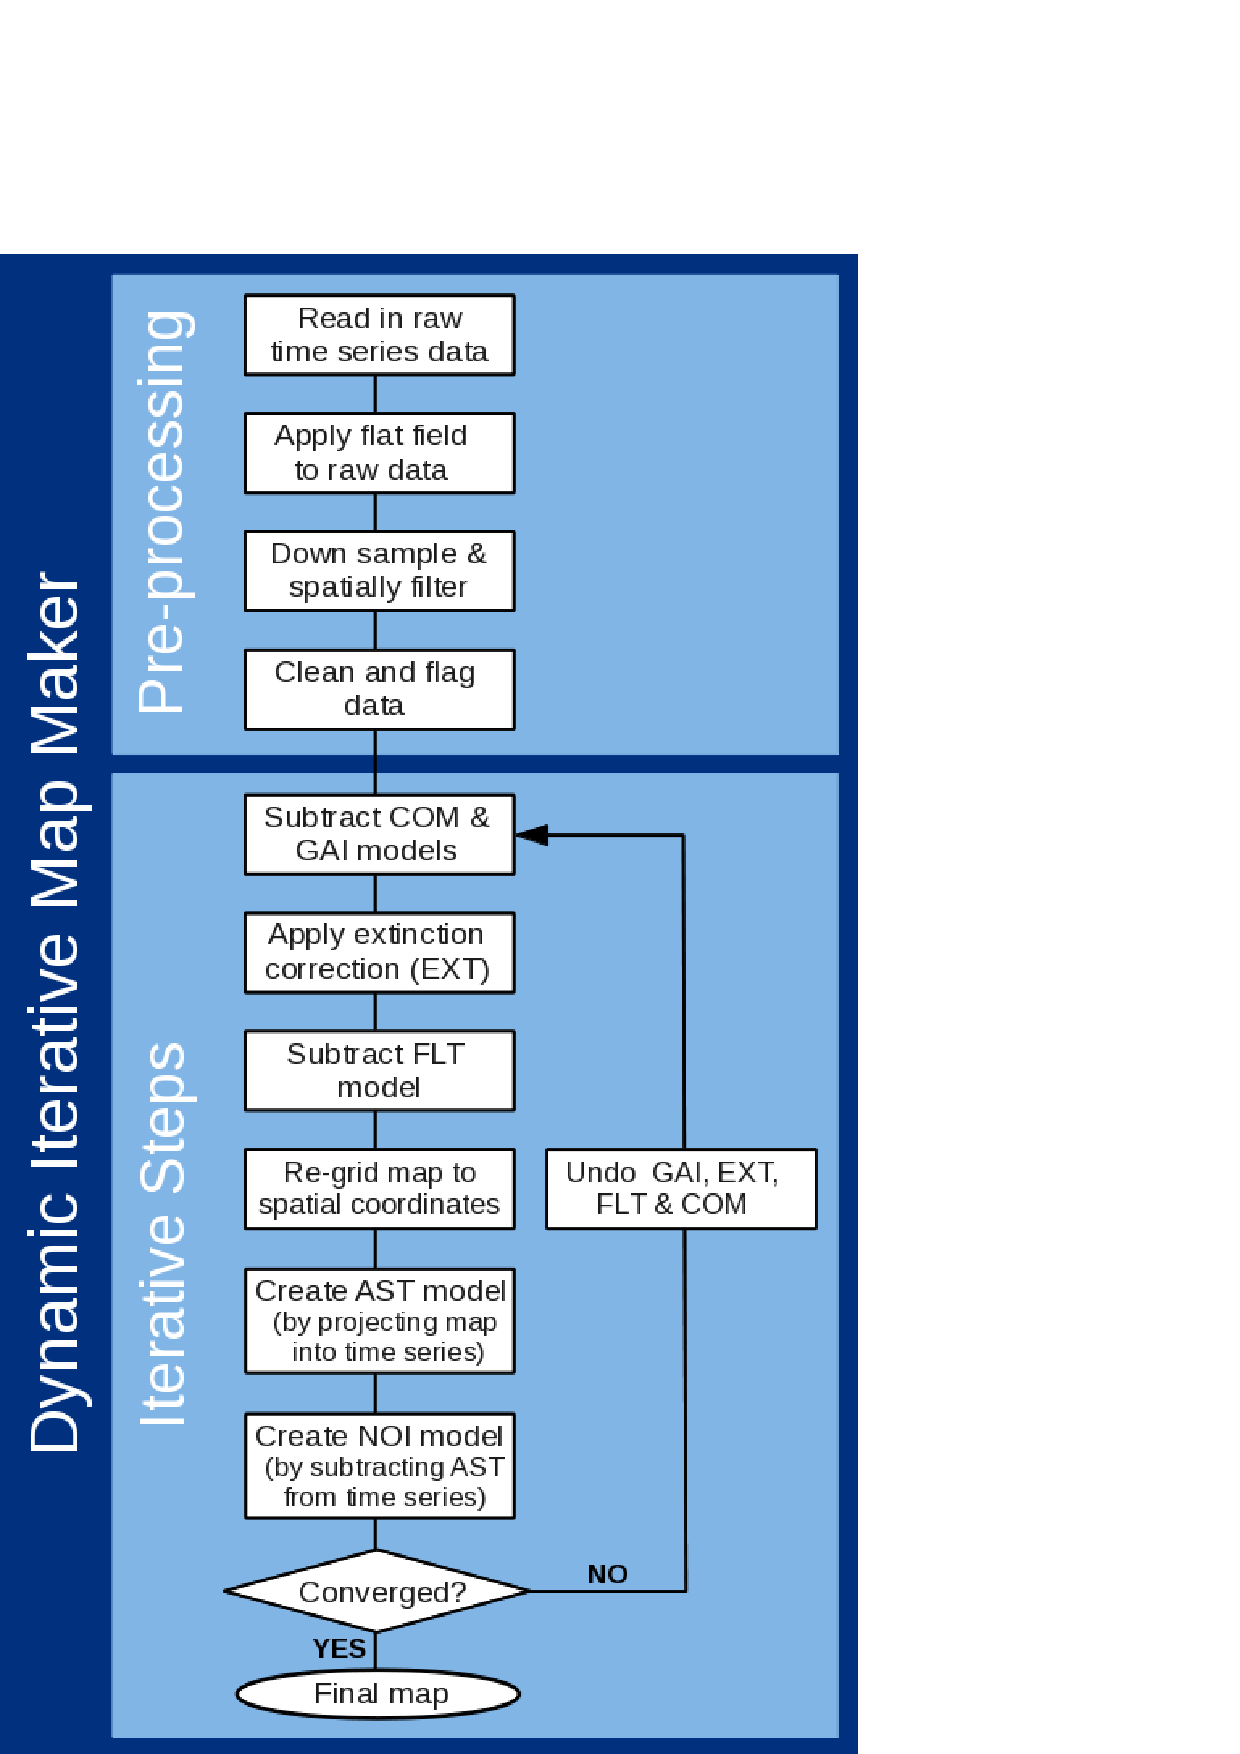
\includegraphics[width=0.78\linewidth]{sc21_flow_dimm_blue}
\typeout{sc21_flow_dimm_blue.eps inserted on page \arabic{page}}
\caption{\label{fig:dimm}\small A flow chart illustrating the dynamic
iterative map-maker. Note that for each iteration the \texttt{AST}
model is subtracted from the time-series leaving only those
contributions to be fitted and removed.}
\end{figure}
\end{latexonly}

% Split into latexonly and htmlonly to obtain correct positioning. and
% to avoid other graphics being interleaved amonst this long, and hence
% divided table.
\begin{latexonly}
\renewcommand*\arraystretch{0.85}

\begin{table*}
\begin{center}
\begin{footnotesize}
\caption{\small The active variables from \texttt{dimmconfig.lis} and their
default values. The third column ('Use') separates the primary parameters commonly
adjusted by users (p), from the secondary parameters only to be adjusted under
caution (s). Neutral parameters (n) do not affect the resulting map. For a fuller
description of each see \cref{Appendix}{app:par_full}{dimmconfig.lis parameters}.
These can also be found in in the default parameter file at
\texttt{https://github.com/Starlink/starlink/blob/master/applications/smurf/defaults/smurf\_makemap.def}.}
\begin{tabular}{|p{2.1cm}|p{0.8cm}|p{0.2cm}|p{11.2cm}|}
\hline
\multicolumn{1}{|l}{Parameter} &\multicolumn{1}{|l}{Value} &\multicolumn{1}{|@{\,}l@{\,}}{Use}& \multicolumn{1}{|l|}{Description\hspace{0.2cm} (see \cref{Appendix}{app:par_full}{this appendix} for full version)} \\
\hline
\multicolumn{4}{|l|}{\textbf{Pre-Processing - General}}\\
\hline
downsampscale & -1 &p &Down-sample to save computer memory and time. Negative value = its
                       magnitude will be multiplied by the PIXSIZE for the
                       requested map.\\

order & 1 &s &Subtract a baseline polynomial of this order\\
badfrac & 0.05 &s& Fraction of samples to be bad to flag entire bolometer
                        as dead\\
flagslow & 30 & p&Flag data taken while telescope was moving so slowly
                        sources sit in $1/f$ noise\\
flagfast & 1000 &p& Flag data taken the telescope was moving too fast causing source
                        smearing\\
pcathresh & 0 &s& PCA cleaning is the threshold above which components
                        will be removed from the bolometer time-series.\\
pcalen & 0 &s &The chunk length that will be cleaned as a number of time slices.\\
compreprocess& 0 &s& If set, include a COM removal in the pre-processing.\\
maxlen& 0 &s &Maximum number of seconds of data to be loaded at once.\\
doclean& 1 &s&Perform pre-processing/cleaning operations. \\
exportclean& 0 &n&If set, the data will be exported after cleaning and before map-making. \\
dcthresh & 25.0 &s& The SNR threshold at which to detect DC step\\
dcfitbox & 30 &s& Box size over which to fit data with a straight
                        line on either side of a potential DC jump\\
dcmaxsteps & 10 &s& The maximum number of steps that can be corrected
                        in each minute of good data.\\
dclimcorr & 0 &s& If more than this number of bolometers have a step at
                        a given time, then all bolometers are corrected for
                        a step.\\
dcsmooth & 50 &s& The width of the median filter used to smooth a
                        bolometer data stream prior to finding DC jump\\
spikethresh & 0 &s& The SNR at which to flag spikes.\\
spikebox & 50 &s& Size of the filter box in which to detect spikes from a rolling median.\\
whiten & 0 &&Whether to apply a whitening filter to time stream data. \\
filt\_edgelow & 0 &s&The highest frequency to be retained by the initial cleaning. \\
 noisecliphigh & 4.0 &s &Reject bolometers noisier than this many standard deviations above the median.\\
 noisecliplow & 0 &s& Reject bolometers noisier than this many standard deviations below the median.\\
 noiseclipprecom & 0 &s &Perform noise clipping before, instead of after, the pre-processing COM removal.\\
\hline
\multicolumn{4}{|l|}{\textbf{Pre-processing - Fake Maps}}\\
\hline
fakemap & undef&- &Diagnostic tool to test the response of the map-maker to known sources.  \\
fakescale & 1 &- &Each pixel in your fakemap will be scaled by this factor. \\


%\textcolor{red}{\hline}
\hline
\multicolumn{4}{|l|}{\textbf{Iterative - General}}\\
\hline
numiter & -5 &p& Number of iterations. A negative number = max iterations if using maptol or $\chi^2$ stopping criteria.\\
maptol & 0.05 &p &The normalised mean change between maps of subsequent iterations. Only used if numiter is negative.\\
modelorder & - &s& =(COM,GAI,EXT,FLT,AST,NOI). which models to include in the iterative process and the order in which they are removed. \\
exportndf & 0 &n& Whether to export all or any of the models. \\
itermap & 0 &n& Whether to write out a map after each iteration.\\
bolomap & 0 &n& Whether to write out a map for each bolometer.\\
shortmap & 0 &n& Whether to write out a map every 'shortmap' time slices.\\
chitol & undef &s& Threshold change in reduced $\chi^2$ in subsequent iterations.\\
varmapmethod & 1 &s& Controls how the map variance values are estimated---either from the time domain noise estimates or the data value in each regridded pixel.\\

\hline
 \multicolumn{4}{|r|}{\emph{Table 2 continued over page}}\\
\hline
\end{tabular}
\label{tab:dimmdef}
\end{footnotesize}
\end{center}
\end{table*}


\begin{table*}
\begin{center}
\begin{footnotesize}
\begin{tabular}{|p{2.3cm}|p{0.8cm}|p{0.2cm}|p{11.0cm}|}
\hline
\multicolumn{4}{|l|}{\emph{Table 2 continued}}\\
\hline
\multicolumn{1}{|l}{Parameter} &\multicolumn{1}{|l}{Value} &\multicolumn{1}{|@{\,}l@{\,}}{Use}& \multicolumn{1}{|l|}{Description \hspace{0.2cm}  (see \cref{Appendix}{app:par_full}{this appendix} for full version)} \\
\hline
\multicolumn{4}{|l|}{\textbf{Iterative - Model Specific}}\\
\hline
com.perarray & 0 &p &Whether to calculate a separate COM model for each sub-array. \\
com.noflag & 0  &s& Enable or disable flagging of bad bolometers using the common-mode.\\
com.corr\_tol & 5  &s& Number of sigma away from mean correlation coefficient tolerance\\
com.corr\_abstol  &  0.2 & s &Lower limit of acceptable correlation between a bolometer time stream and the common-mode. \\

com.gain\_tol & 5  &s& Number of sigma away from mean gain coefficient tolerance\\
com.gain\_abstol & 3  &s& Maximum absolute ratio between a bolometers gain and the mean gain.\\
com.gain\_box &-30.0 &s & The number of time slices (or seconds if negative)
                          in a box\\
com.gain\_fgood & 0.25 &s &Minimum fraction of good gain boxes for bolometer not to be rejected. \\
com.gain\_rat & 4.0  &s&Ratio of the largest gain to the mean gain for a bolometer not to be rejected. \\

com.zero\_mask & 0  &s&Use if wish to provide an external COM mask. Must specify this on the command-line using the REF option.  \\
com.zero\_circle & undef &s &Use to set a circular mask; any samples within the mask are excluded from the COM estimation. \\
com.zero\_lowhits & 0  &s&Samples are excluded from the COM estimation if they fall where the number of samples exceeds this number times the mean. \\
com.zero\_snr & 0 & s&Samples are excluded from the COM estimation if they fall in pixels with SNR values greater than com.zero\_snr. \\
com.zero\_snrlo & 0  &s& Allows the mask of com.zero\_snr to expand down an SNR of com.zero\_snrlo.\\
com.zero\_union & 1 &s & Details how to combine multiple COM masks. \\
com.zero\_freeze & 0 &s & Specifies whether the COM model should be frozen after com.zero\_freeze number of iterations. \\



\hline
noi.calcfirst & 0 & s&Specifies whether to determine the bolometers weights before or after the first iteration.\\
noi.box\_size & 0 &p &The number of time slices to use to determine the noise levels in the time stream. 0 = full bolometer time stream used.\\

\hline
450.flt.filt\_edge-  & \multirow{2}{*}{600} &\multirow{2}{*}{p} & \multirow{4}{*}{{\Huge$\rbrace$}
                         \begin{minipage}{10.3cm}Apply a frequency filter to the
                         FLT model. The value is given in arcsecs which the
                         map-maker converts to frequency.\end{minipage} }\\
\_largescale&  && \\
850.flt.filt\_edge- & \multirow{2}{*}{300}  &\multirow{2}{*}{p}& \\
\_largescale& & & \\
flt.notfirst & 0 &s & Whether to apply the high pass filter filter on the first iteration.\\
flt.zero\_mask & 0 &p & Use if wish to provide an external FLT mask. Must specify this on the command-line using the REF option.\\
flt.zero\_circle & undef  &p&Use to set a circular mask; any samples within the mask are excluded from the filtering. \\
flt.zero\_lowhits & 0 &p & Samples are excluded from the filtering if they fall where the number of samples exceeds this number times the mean. \\
flt.zero\_snr &0 &p &Samples are excluded from the filtering if they lie in pixels with SNR values greater than flt.zero\_snr. \\
flt.zero\_snrlo & 0   &p& Allows the mask of flt.zero\_snr to expand down an SNR of flt.zero\_snrlo.\\
flt.zero\_union & 1  &p&Details how to combine multiple FLT masks. \\
flt.zero\_freeze & 0  &p&Specifies whether the FLT model should be frozen after flt.zero\_freeze number of iterations.  \\
flt.zero\_niter & 2  &p& The number of iterations for which the FLT model should be masked.\\

\hline

ext.csotau & undef &s &Specifies the CSO tau value to be used. \\
ext.filtertau & undef &s & Used if ext.tausrc=filtertau. \\

ext.tausrc & auto  &s& Options = auto, wvmraw, csotau, filtertau\\
ext.taumethod & adapt  &s& Options = adaptive, full, quick\\
\hline
ast.mapspike & 10  &s&Removes spikes from the map by removing residuals in each pixel above ast.mapspike standard deviations above the mean. \\
ast.zero\_mask  & 0 &p &Use if wish to provide an external AST mask. Must specify this on the command-line. \\

\hline
 \multicolumn{4}{|r|}{\emph{Table 2 continued over page}}\\
\hline
\end{tabular}
\end{footnotesize}
\end{center}
\end{table*}


\begin{table*}
\begin{center}
\begin{footnotesize}
\begin{tabular}{|p{2.5cm}|p{0.6cm}|p{0.2cm}|p{11.0cm}|}
\hline
\multicolumn{4}{|l|}{\emph{Table 2 continued}}\\
\hline
\multicolumn{1}{|l}{Parameter} &\multicolumn{1}{|l}{Value} &\multicolumn{1}{|@{\,}l@{\,}}{Use}& \multicolumn{1}{|l|}{Description \hspace{0.2cm} (see \cref{Appendix}{app:par_full}{this appendix} for full version)} \\
\hline
ast.zero\_circle  & undef&p&Use to set a circular mask; any samples outside the mask will be constrained to zero on each iteration. \\
ast.zero\_lowhits & 0  &p& Forces the map to zero where the number of samples is less than this number times the mean.\\
ast.zero\_snr  & 0 &p & Creates a mask after each iteration based on the SNR of the pixels. Map areas outside this mask will be forced to zero.\\
ast.zero\_snrlo  & 0 & p& Allows the mask of ast.zero\_snr to expand down an SNR of ast.zero\_snrlo.\\
ast.zero\_snr\_fwhm & 0 & s&The FWHM by which to smooth the AST mask created by ast.zero\_snr. The map-maker is then run again using this smoothed mask on each iteration.  \\
ast.zero\_snr\_low &-1.1&s & The value at which to threshold the smooth mask produced by ast.zero\_snr\_fwhm.\\
ast.zero\_union & 1  &p&Details how to combine multiple AST masks. \\
ast.zero\_freeze & 0 &p & Specifies whether the AST model should be frozen after ast.zero\_freeze number of iterations. \\
\hline
\end{tabular}

\end{footnotesize}
\end{center}
\end{table*}

\renewcommand*\arraystretch{1.0}
\end{latexonly}

\subsection{\xlabel{dimm_theory}The theory}
\label{sec:dimm_theory}

The map-maker works by individually modelling the various
contributions that make up the signal recorded by each bolometer. It
models and then subtracts all the sources of signal in order of
decreasing magnitude, ultimately leaving just the astronomical signal
plus noise. A list of the modelled components can be seen in
\cref{Table}{tab:mods}{tabulated} and a description found in
\cref{Section}{sec:models}{The Individual Models}.
% tab:mods references the section sec:models not the table in PostScript.
% Reason TBD.

The map-maker calls configuration parameters which instruct the
map-maker on the pre-processing steps, which components to iteratively
model, the parameters to use when doing so, and the stopping (or
convergence) criteria. There is single `master' file which contains
\emph{all} the parameters available for use by the map-maker. This
file can be found in your \smurf\ path or online at the \starlink\
\htmladdnormallink{github repository}{https://github.com/Starlink/starlink/blob/master/applications/smurf/defaults/smurf\_makemap.def}
\latex{\footnote{\texttt{https://github.com/Starlink/starlink/blob/master/applications/smurf/defaults/smurf\_makemap.def}}}
 and is fully documented.

The default parameters alone will not make an optimal map. A
configuration file, to be specified on the command line, must
accompany each reduction. The default configuration file called by
users when running \makemap\ is \texttt{dimmconfig.lis}. This file
contains the most important parameters to users (and ultimately the
parameters which should be adjusted by users should they wish). These
parameters are given in \cref{Table}{tab:dimmdef}{a following table}
while a full description of each can be found in
\cref{Appendix}{app:par_full}{an appendix}.

Often, the default configuration file (\texttt{dimmconfig.lis}) will
not give optimal results for your particular observation. For this
reason, specialised configuration files have been developed which are
tailored to different science goals, be they detecting faint galaxies
or mapping large molecular clouds. A description of these specialised
configuration files can be found \cref{in Section}{sec:config}{here}.
\\ \\
{\large{\texttt{\bf dimmconfig.lis}}}\\
\cref{Figure}{fig:dimm}{The graphic below} shows the flow chart
of the map making process
for \texttt{dimmconfig.lis}. It is divided into two sections: the
pre-processing stage where the data are cleaned, then the iterative
stage where the different models are subtracted.
\cref{Table}{tab:dimmdef}{A table of active variables} gives all the
configuration parameters in \texttt{dimmconfig.lis} again, divided
into the two main stages.

%\begin{htmlonly}
%\myfig{sc21_flow_dimm_blue}{}{width=0.78\linewidth}{fig:dimm}{
%  A flow chart illustrating the dynamic iterative map-maker. Note that
%  for each iteration the \texttt{AST} model is subtracted from the
%  time-series leaving only those contributions to be fitted and
%  removed.}
%\end{htmlonly}

\begin{htmlonly}
\label{fig:dimm} \htmladdimg{sc21_flow_dimm_blue.png}\\
    \\
    Figure: A flow chart illustrating the dynamic iterative map-maker.
    Note that for each iteration the \texttt{AST} model is subtracted
    from the time-series leaving only those contributions to be fitted
    and removed.\\
    }
\end{htmlonly}

The first task the map-maker performs is to down-sample the data. The
raw time-series data is re-sampled at a rate that matches the
requested pixel size, the equivalent to applying a low-pass filter.
Down-sampling saves time and memory usage when running the map-maker.
The raw data is then concatenated and has the flat-field (from the
bracketing fast flat scans) applied to calibrate the bolometers. A
number of cleaning steps are then run: a polynomial baseline is
subtracted from each bolometer; spikes and dc steps are removed; any
resulting gaps in the time-series are filled in.

Next comes the iterative stage of the process. First to be modelled
and removed are \texttt{COM} and \texttt{GAI} which work together to
calculate the average signal template of all the bolometers, and then
fit/remove the templates from each bolometer. The next model
(\texttt{EXT}) applies a multiplicative extinction correction to the
data. Following this, a Fourier transform is applied to the data and
the \texttt{FLT} model is removed in the frequency domain.
\texttt{FLT} applies a high-pass filter to the data, above frequencies
that correspond to angular scales of 600\,arcsec and 300\,arcsec at
450$\mu$m and 850$\mu$m, respectively.

Next comes the \texttt{AST} model, the first step of which involves
regridding the data to produce an estimation of the final science map.
Since many samples typically contribute to the estimate of the signal
in a given pixel, the noise is greatly reduced compared with the
time-series data. This map is then projected back into the time series
and the \texttt{AST} model removed. The \texttt{NOI} model then
measures the noise in the residual signals for each bolometer to
establish weights for the data as they are placed into the map in
subsequent iterations.

At this stage convergence is checked against the parameters detailed
in the configuration file. Convergence is achieved either when the
requested number of iterations has been completed or when the
noise-based convergence criteria specified in the configuration file
is reached. If more iterations are required or (in the latter case)
the residual noise has not converged then \texttt{GAI}, \texttt{EXT},
\texttt{FLT} and \texttt{COM} models are all undone and the
time-series is reconstructed. The sequence is then rerun only this
time without \texttt{AST} complicating the model fitting.

\begin{htmlonly}
\setlength{\extrarowheight}{3pt}
\begin{table}
\centering
\begin{tabular}{c|l}
\hline
\textbf{Model} &\hspace{0.2cm} \textbf{Description} \\
\hline
\texttt{COM}&\hspace{0.2cm} Common-mode signal\\
\texttt{GAI}&\hspace{0.2cm} Common-mode scaled to each bolometer---the gain\\
\texttt{EXT}&\hspace{0.2cm} Extinction correction\\
\texttt{FLT}&\hspace{0.2cm} Fourier transform filter\\
\texttt{AST}&\hspace{0.2cm} Map estimate of astronomical signal\\
\texttt{NOI}&\hspace{0.2cm} Noise estimation\\
\hline
\end{tabular}
\label{tab:mods}
\caption{\small Table adopted from Chapin et al. (2013). A fuller
explanation of each model is given below.}
\end{table}
\end{htmlonly}

\raggedbottom
\subsection{\xlabel{models}The individual models}
\label{sec:models}

% Split to obtain sensible position of table in the PostScript.
\begin{latexonly}
\setlength{\extrarowheight}{3pt}
\begin{table}[t!]
\centering
\begin{tabular}{c|l}
\hline
\textbf{Model} &\hspace{0.2cm} \textbf{Description} \\
\hline
\texttt{COM}&\hspace{0.2cm} Common-mode signal\\
\texttt{GAI}&\hspace{0.2cm} Common-mode scaled to each bolometer---the gain\\
\texttt{EXT}&\hspace{0.2cm} Extinction correction\\
\texttt{FLT}&\hspace{0.2cm} Fourier transform filter\\
\texttt{AST}&\hspace{0.2cm} Map estimate of astronomical signal\\
\texttt{NOI}&\hspace{0.2cm} Noise estimation\\
\hline
\end{tabular}
\label{tab:mods}
\caption{\small Table adopted from Chapin et al. (2013). A fuller
explanation of each model is given below.}
\end{table}
\end{latexonly}

The particular sequence of the models evaluated (and removed) by the
map-maker during the iterative stage is indicated by the
\texttt{modelorder} parameter in the configuration file. These models
are modular however so their order may be changed. The default model
order in \texttt{dimmconfig.lis} is given below.
\vspace{-0.1cm}
\begin{myquote}
\begin{verbatim}
modelorder = (com,gai,ext,flt,ast,noi)
\end{verbatim}
\end{myquote}
\vspace{-0.1cm}
The only recipe not following this model order is the one tailored for
blank field maps which does not include a \texttt{FLT} model in the
iterative stage (see \cref{Section}{sec:config}{Specialised
configuration files}). Below is a basic
description of each model, while more complete descriptions of the
models and all the associated caveats can be found in Chapin et al.
(2013) \cite{mapmaker}.
\\ \\
\begin{minipage}[t]{0.07\linewidth}
\texttt{COM}
\end{minipage}
\begin{minipage}[t]{0.92\linewidth}The \texttt{COM} model removes the
common-mode signal (the signal that is common to all bolometers), the
dominant contributor to this signal being the sky noise. It determines
this by simply averaging over all bolometers for each time slice.
Bolometers are flagged as bad, (and thus omitted from the final map), if
they do not resemble the \texttt{COM} model seen by the majority of the
other bolometers.
\newline Extended emission on a scale larger than the array footprint
on the sky will contribute a signal indistinguishable from a
common-mode signal. This puts an upper limit on the spatial scale of
astronomical emission that can be recovered. \\
\end{minipage}

\begin{minipage}[t]{0.07\linewidth}
\texttt{GAI}
\end{minipage}
\begin{minipage}[t]{0.92\linewidth}The \texttt{GAI} model works with
\texttt{COM} in removing the common-mode signal. \texttt{GAI} is used to
scale the \texttt{COM} model that has been subtracted and is described by
a gain and an offset to scale all the bolometers to the same level. This
will allow the bolometers to share a common calibration further down the
line. \\
\end{minipage}
\begin{minipage}[t]{0.07\linewidth}
\texttt{EXT}
\end{minipage}
\begin{minipage}[t]{0.92\linewidth}\texttt{EXT} applies the extinction
correction. This is a time-varying scaling factor that is derived from
the JCMT water-vapour radiometer. As it deals with 30-second chunks of
data this accounts for varying conditions over a long observation. For
more details see \cref{Appendix}{app:cal}{SCUBA-2 data calibration}. \\
\end{minipage}
\begin{minipage}[t]{0.07\linewidth}
\texttt{FLT}
\end{minipage}
\begin{minipage}[t]{0.92\linewidth}The \texttt{FLT} model acts on the FFT
of the bolometer data. High-pass (only allows \emph{higher} frequencies to
pass) and low-pass (only allows \emph{lower} frequencies to pass) filters
can be specified. These cut-off frequencies can either be be specified by
you directly or as an angular spatial scale (which is subsequently
converted into a frequency dependent on the speed at which the
telescope is moving). The most important role of this model is to
apply a high-pass filter in order to remove the $1/f$ noise. Note that
extended emission varies slowly over the array; it therefore appears
at low frequencies and complicates the choice of a high-pass filter. A
further discussion of this matter is given in
\cref{Section}{sec:bright_ex}{Extended galactic sources}\\
\end{minipage}
\begin{minipage}[t]{0.07\linewidth}
\texttt{AST}
\end{minipage}
\begin{minipage}[t]{0.92\linewidth}This step involves both the creation of the
\texttt{AST} model and the final science map. Hence, the position of
\texttt{AST} in the model order indicates at what stage the astronomical
image should be estimated. When the \texttt{AST} model is called, the first
step is regridding the raw time-series data, (using nearest-neighbour sampling),
to produce an estimate of the final map. Following this, the map is
projected back into the time domain and removed (as the \texttt{AST}
model).\\
\end{minipage}
\begin{minipage}[t]{0.07\linewidth}
\texttt{NOI}
\end{minipage}
\begin{minipage}[t]{0.92\linewidth}\texttt{NOI} should come last in the model
order and calculates the noise in each bolometer on the first iteration only. \texttt{NOI} is
determined by running \calcnoise\ (see \cref{Section}{sec:calcnoise}{Checking the
array performance}) on the residual signal (the \texttt{RES} model, see
\cref{Section}{sec:export}{Exporting individual models}) and taking the noise
between 2 and 10\,Hz. Unlike the other models, \texttt{NOI} is not a subtraction or
a correction but, if specified, is used to weight the bolometers on subsequent iterations.
\end{minipage}

% Needed because latex2html seems unable to handle multirow
\begin{htmlonly}
\begin{table*}
\begin{center}
\begin{footnotesize}

\begin{tabular}{|p{2.1cm}|p{0.8cm}|p{0.2cm}|p{11.2cm}|}
\hline
\multicolumn{1}{|l}{Parameter} &\multicolumn{1}{|l}{Value} &\multicolumn{1}{|@{\,}l@{\,}}{Use}& \multicolumn{1}{|l|}{Description\hspace{0.2cm}  (see \cref{Appendix}{app:par_full}{this appendix} for full version)} \\
\hline
\multicolumn{4}{|l|}{\textbf{Pre-Processing - General}}\\
\hline
downsampscale & -1 &p &Down-sample to save computer memory and time. Negative value = its
                       magnitude will be multiplied by the PIXSIZE for the
                       requested map.\\

order & 1 &s &Subtract a baseline polynomial of this order\\
badfrac & 0.05 &s& Fraction of samples to be bad to flag entire bolometer
                        as dead\\
flagslow & 30 & p&Flag data taken while telescope was moving so slowly
                        sources sit in $1/f$ noise\\
flagfast & 1000 &p& Flag data taken the telescope was moving too fast causing source
                        smearing\\
pcathresh & 0 &s& PCA cleaning is the threshold above which components
                        will be removed from the bolometer time-series.\\
pcalen & 0 &s &The chunk length that will be cleaned as a number of time slices.\\
compreprocess& 0 &s& If set, include a COM removal in the pre-processing.\\
maxlen& 0 &s &Maximum number of seconds of data to be loaded at once.\\
doclean& 1 &s&Perform pre-processing/cleaning operations. \\
exportclean& 0 &n&If set, the data will be exported after cleaning and before map-making. \\
dcthresh & 25.0 &s& The SNR threshold at which to detect DC step\\
dcfitbox & 30 &s& Box size over which to fit data with a straight
                        line on either side of a potential DC jump\\
dcmaxsteps & 10 &s& The maximum number of steps that can be corrected
                        in each minute of good data.\\
dclimcorr & 0 &s& If more than this number of bolometers have a step at
                        a given time, then all bolometers are corrected for
                        a step.\\
dcsmooth & 50 &s& The width of the median filter used to smooth a
                        bolometer data stream prior to finding DC jump\\
spikethresh & 0 &s& The SNR at which to flag spikes.\\
spikebox & 50 &s& Size of the filter box in which to detect spikes from a rolling median.\\
whiten & 0 &&Whether to apply a whitening filter to time-stream data. \\
filt\_edgelow & 0 &s&The highest frequency to be retained by the initial cleaning. \\
 noisecliphigh & 4.0 &s &Reject bolometers noisier than this many standard deviations above the median.\\
 noisecliplow & 0 &s& Reject bolometers noisier than this many standard deviations below the median.\\
 noiseclipprecom & 0 &s &Perform noise clipping before, instead of after, the pre-processing COM removal.\\
\hline
\multicolumn{4}{|l|}{\textbf{Pre-processing - Fake Maps}}\\
\hline
fakemap & undef&- &Diagnostic tool to test the response of the map-maker to known sources.  \\
fakescale & 1 &- &Each pixel in your fakemap will be scaled by this factor. \\
\hline
\multicolumn{4}{|l|}{\textbf{Iterative - General}}\\
\hline
numiter & -5 &p& Number of iterations. A negative number = max iterations if using maptol or $\chi^2$ stopping criteria\\
maptol & 0.05 &p &The normalised mean change between maps of subsequent iterations. Only used if numiter is negative.\\
modelorder & - &s& =(COM,GAI,EXT,FLT,AST,NOI). which models to include in the iterative process and the order in which they are removed. \\
exportndf & 0 &n& Whether to export all or any of the models. \\
itermap & 0 &n& Whether to write out a map after each iteration.\\
bolomap & 0 &n& Whether to write out a map for each bolometer.\\
shortmap & 0 &n& Whether to write out a map every 'shortmap' time slices.\\
chitol & undef &s& Threshold change in reduced $\chi^2$ in subsequent  iterations.\\
varmapmethod & 1 &s& Controls how the map variance values are estimated---either from the time domain noise estimates or the data value in each regridded pixel.\\
\hline
\multicolumn{4}{|l|}{\textbf{Iterative - Model Specific}}\\
\hline
com.perarray & 0 &p &Whether to calculate a separate COM model for each sub-array. \\
com.noflag & 0  &s& Enable or disable flagging of bad bolometers using the common-mode.\\
com.corr\_tol & 5  &s& Number of sigma away from mean correlation coefficient tolerance\\
com.corr\_abstol  &  0.2 & s &Lower limit of acceptable correlation between a bolometer time stream and the common-mode. \\

com.gain\_tol & 5  &s& Number of sigma away from mean gain coefficient tolerance\\
com.gain\_abstol & 3  &s& Maximum absolute ratio between a bolometers gain and the mean gain.\\
com.gain\_box &-30.0 &s & The number of time slices (or seconds if negative)
                          in a box\\
com.gain\_fgood & 0.25 &s &Minimum fraction of good gain boxes for bolometer not to be rejected. \\
com.gain\_rat & 4.0  &s&Ratio of the largest gain to the mean gain for a bolometer not to be rejected. \\

com.zero\_mask & 0  &s&Use if wish to provide an external COM mask. Must specify this on the command-line using the REF option.  \\
com.zero\_circle & undef &s &Use to set a circular mask; any samples within the mask are excluded from the COM estimation. \\
com.zero\_lowhits & 0  &s&Samples are excluded from the COM estimation if they fall where the number of samples exceeds this number times the mean. \\
com.zero\_snr & 0 & s&Samples are excluded from the COM estimation if they fall in pixels with SNR values greater than com.zero\_snr. \\
com.zero\_snrlo & 0  &s& Allows the mask of com.zero\_snr to expand down an SNR of com.zero\_snrlo.\\
com.zero\_union & 1 &s & Details how to combine multiple COM masks. \\
com.zero\_freeze & 0 &s & Specifies whether the COM model should be frozen after com.zero\_freeze number of iterations. \\
\hline
noi.calcfirst & 0 & s&Specifies whether to determine the bolometers weights before or after the first iteration.\\
noi.box\_size & 0 &p &The number of time slices to use to determine the noise levels in the time stream. 0 = full bolometer time stream used.\\
\hline
450.flt.filt\_edge\_largescale  & 600 &p & Apply a frequency filter to the FLT model at 450\,$\mu$m. The value is given in arcsecs which the  map-maker converts to frequency.\\
850.flt.filt\_edge\_largescale &300  &p& Apply a frequency filter to the FLT model at 850\,$\mu$m. The value is given in arcsecs which the  map-maker converts to frequency.\\
flt.notfirst & 0 &s & Whether to apply the high pass filter filter on the first iteration.\\
flt.zero\_mask & 0 &p & Use if wish to provide an external FLT mask. Must specify this on the command-line using the REF option.\\
flt.zero\_circle & undef  &p&Use to set a circular mask; any samples within the mask are excluded from the filtering. \\
flt.zero\_lowhits & 0 &p & Samples are excluded from the filtering if they fall where the number of samples exceeds this number times the mean. \\
flt.zero\_snr &0 &p &Samples are excluded from the filtering if they lie in pixels with SNR values greater than flt.zero\_snr. \\
flt.zero\_snrlo & 0   &p& Allows the mask of flt.zero\_snr to expand down an SNR of flt.zero\_snrlo.\\
flt.zero\_union & 1  &p&Details how to combine multiple FLT masks. \\
flt.zero\_freeze & 0  &p&Specifies whether the FLT model should be frozen after flt.zero\_freeze number of iterations.  \\
flt.zero\_niter & 2  &p& The number of iterations for which the FLT model should be masked.\\

\hline

ext.csotau & undef &s &Specifies the CSO tau value to be used. \\
ext.filtertau & undef &s & Used if ext.tausrc=filtertau. \\

ext.tausrc & auto  &s& Options = auto, wvmraw, csotau, filtertau\\
ext.taumethod & adapt  &s& Options = adaptive, full, quick\\
\hline
ast.mapspike & 10  &s&Removes spikes from the map by removing residuals in each pixel above ast.mapspike standard deviations above the mean. \\
ast.zero\_mask  & 0 &p &Use if wish to provide an external AST mask. Must specify this on the command-line. \\
ast.zero\_circle  & undef&p&Use to set a circular mask; any samples outside the mask will be constrained to zero on each iteration. \\
ast.zero\_lowhits & 0  &p& Forces the map to zero where the number of samples is less than this number times the mean.\\
ast.zero\_snr  & 0 &p & Creates a mask after each iteration based on the SNR of the pixels. Map areas outside this mask will be forced to zero.\\
ast.zero\_snrlo  & 0 & p& Allows the mask of ast.zero\_snr to expand down an SNR of ast.zero\_snrlo.\\
ast.zero\_snr\_fwhm & 0 & s&The FWHM by which to smooth the AST mask created by ast.zero\_snr. The map-maker is then run again using this smoothed mask on each iteration.  \\
ast.zero\_snr\_low &-1.1&s & The value at which to threshold the smooth mask produced by ast.zero\_snr\_fwhm.\\
ast.zero\_union & 1  &p&Details how to combine multiple AST masks. \\
ast.zero\_freeze & 0 &p & Specifies whether the AST model should be frozen after ast.zero\_freeze number of iterations. \\
\hline
\end{tabular}
\label{tab:dimmdef}
\caption{\small The active variables from \texttt{dimmconfig.lis} and their
default values. For a fuller description of each, as well as other
options, see \cref{Appendix}{app:par_full}{Configuration Parameters: dimmconfig.lis}.}
\end{footnotesize}
\end{center}
\end{table*}
\end{htmlonly}


\subsection{\xlabel{convergence}Convergence}
\label{sec:converge}

The convergence criteria is crucial to the success of the iterative
process. Convergence is achieved when the requested number of
iterations has been completed \textbf{OR} when the convergence
criteria specified in the configuration file is reached.

Specifying the number of iterations in the configuration file is done via
the \texttt{numiter} parameter. In \texttt{dimmconfig.lis}, this is given
by:
\vspace{-0.1cm}
\begin{myquote}
\begin{verbatim}
numiter = -5
\end{verbatim}
\end{myquote}
\vspace{-0.2cm}
A positive value for \texttt{numiter} means that the requested number
of iterations will be executed. A negative value, as in the example
above, indicates that no more than this number of iterations should be
performed, \emph{but} that it may stop at fewer if convergence
(according to the noise criteria below) has been achieved.

There are two parameters in the configuration file for specifying a
convergence criteria based on noise:
\\ \\
\begin{minipage}[t]{0.1\linewidth}
\texttt{maptol}
\end{minipage}
\begin{minipage}[t]{0.9\linewidth}
This is the average normalised change in the value of map pixels
between subsequent iterations. Convergence is reached when the change
is less than the parameter \texttt{maptol}. It has units of the noise
in the map, thus \texttt{maptol}$=$0.05 means a change of
$<$0.05\,$\sigma$. This option has the advantage of directly assessing
the noise in the resulting map rather than the time-series.
\vspace{3mm}\\
Typically the normalized change in pixel values between iterations
drops rapidly to begin with and then flattens out, decreasing
increasingly slowly. As a result, in some circumstances, the map-maker
will fail to stop iterating due to low frequency ripples coming and
going between iterations.
\vspace{3mm}\\
\texttt{maptol} = 0.05 is the default all recipes. Be aware that
setting \texttt{maptol} to lower than 0.05 will dramatically increase
the length of time to produce the final map and possibly never achieve
convergence. [RECOMMENDED]
\end{minipage}
\vspace{2mm}

\begin{minipage}[t]{0.1\linewidth}
\texttt{chitol}
\end{minipage}
\begin{minipage}[t]{0.9\linewidth}This alternative convergence criteria checks
the change in the reduced chi-squared, $\chi^2$, with the standard deviations
being measured for each of the residual bolometers signals once all the
model components have been removed. Note that it is the noise in the
time-series data that is being checked. The map has converged once the
the change in consecutive values of $\chi^2$ is less than the
parameter \texttt{chitol}.
\vspace{3mm}
\end{minipage}

The best way of checking the progress of convergence while running the
map-maker is to use the \param{itermap} option and setting
\param{itermap = 1} (see \cref{Section}{sec:tweak}{Tweaking the
Configuration File}).


\subsection{\xlabel{export}Exporting individual models}
\label{sec:export}

% Split to obtain sensible position of table in the PostScript.
\begin{latexonly}
\begin{figure}[t!]
\begin{center}
  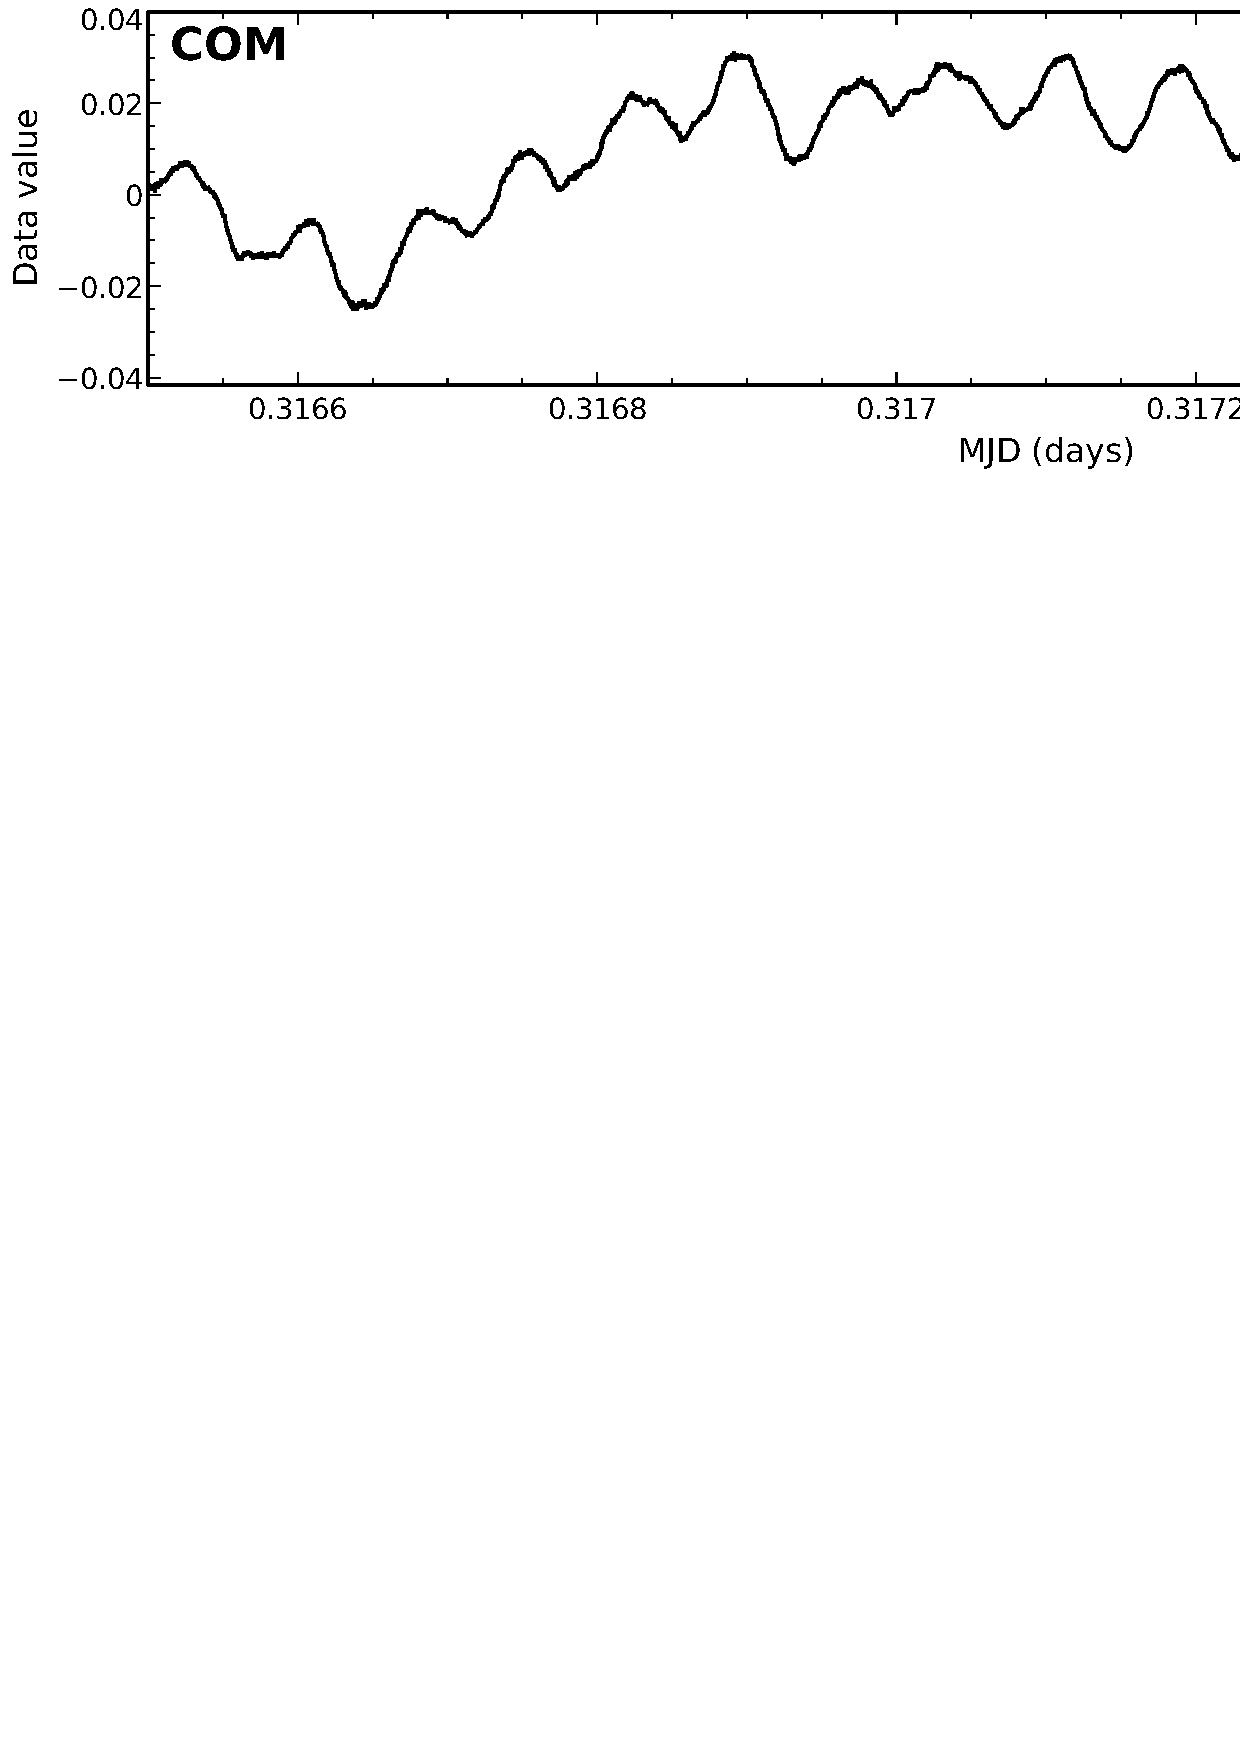
\includegraphics[width=\linewidth]{sc21_com} \\
  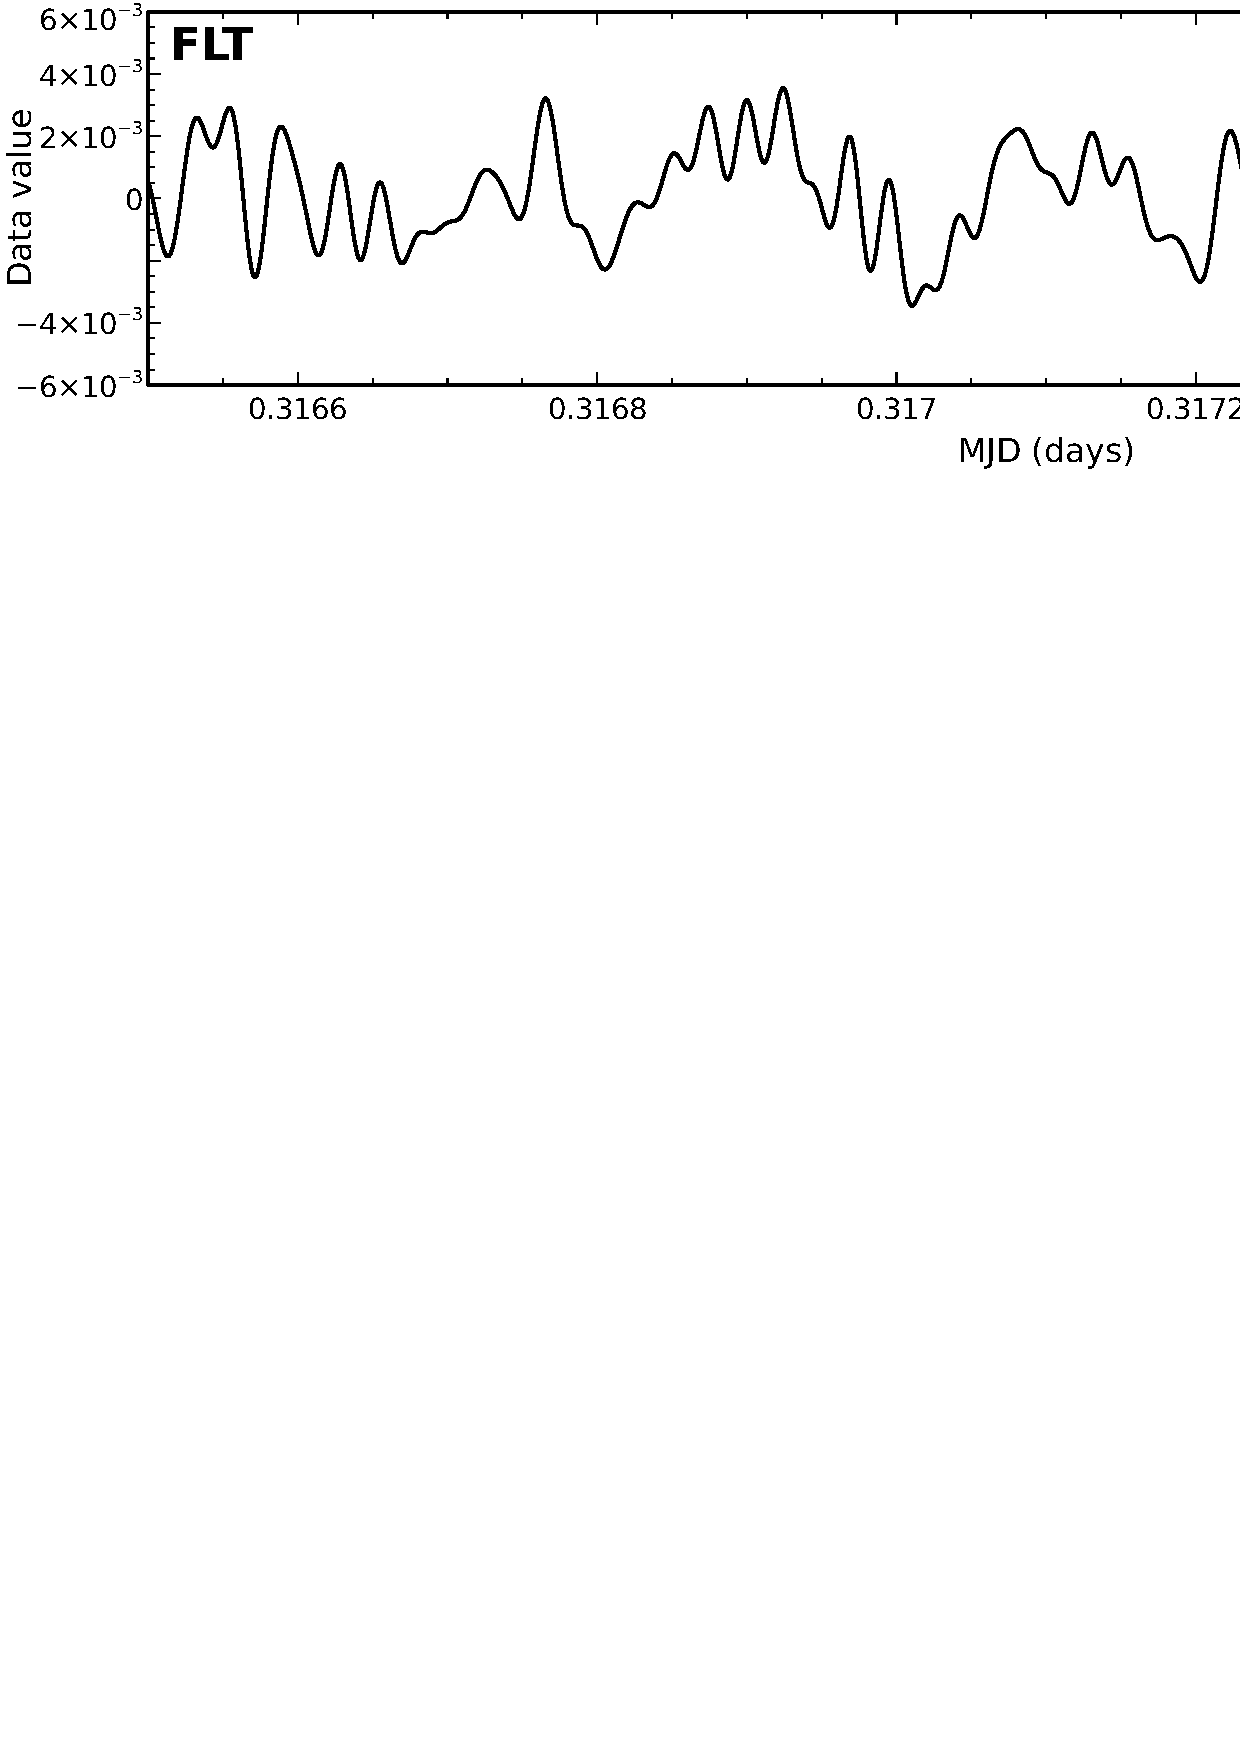
\includegraphics[width=\linewidth]{sc21_flt} \\
  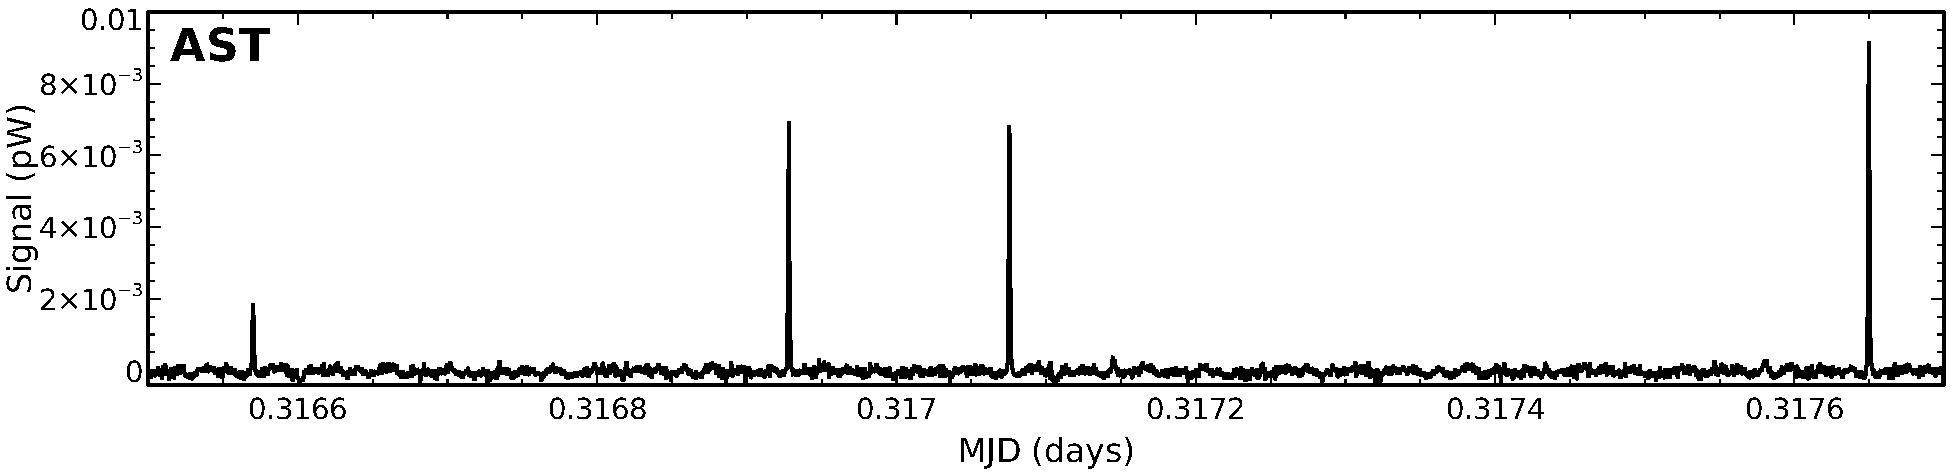
\includegraphics[width=\linewidth]{sc21_ast} \\
  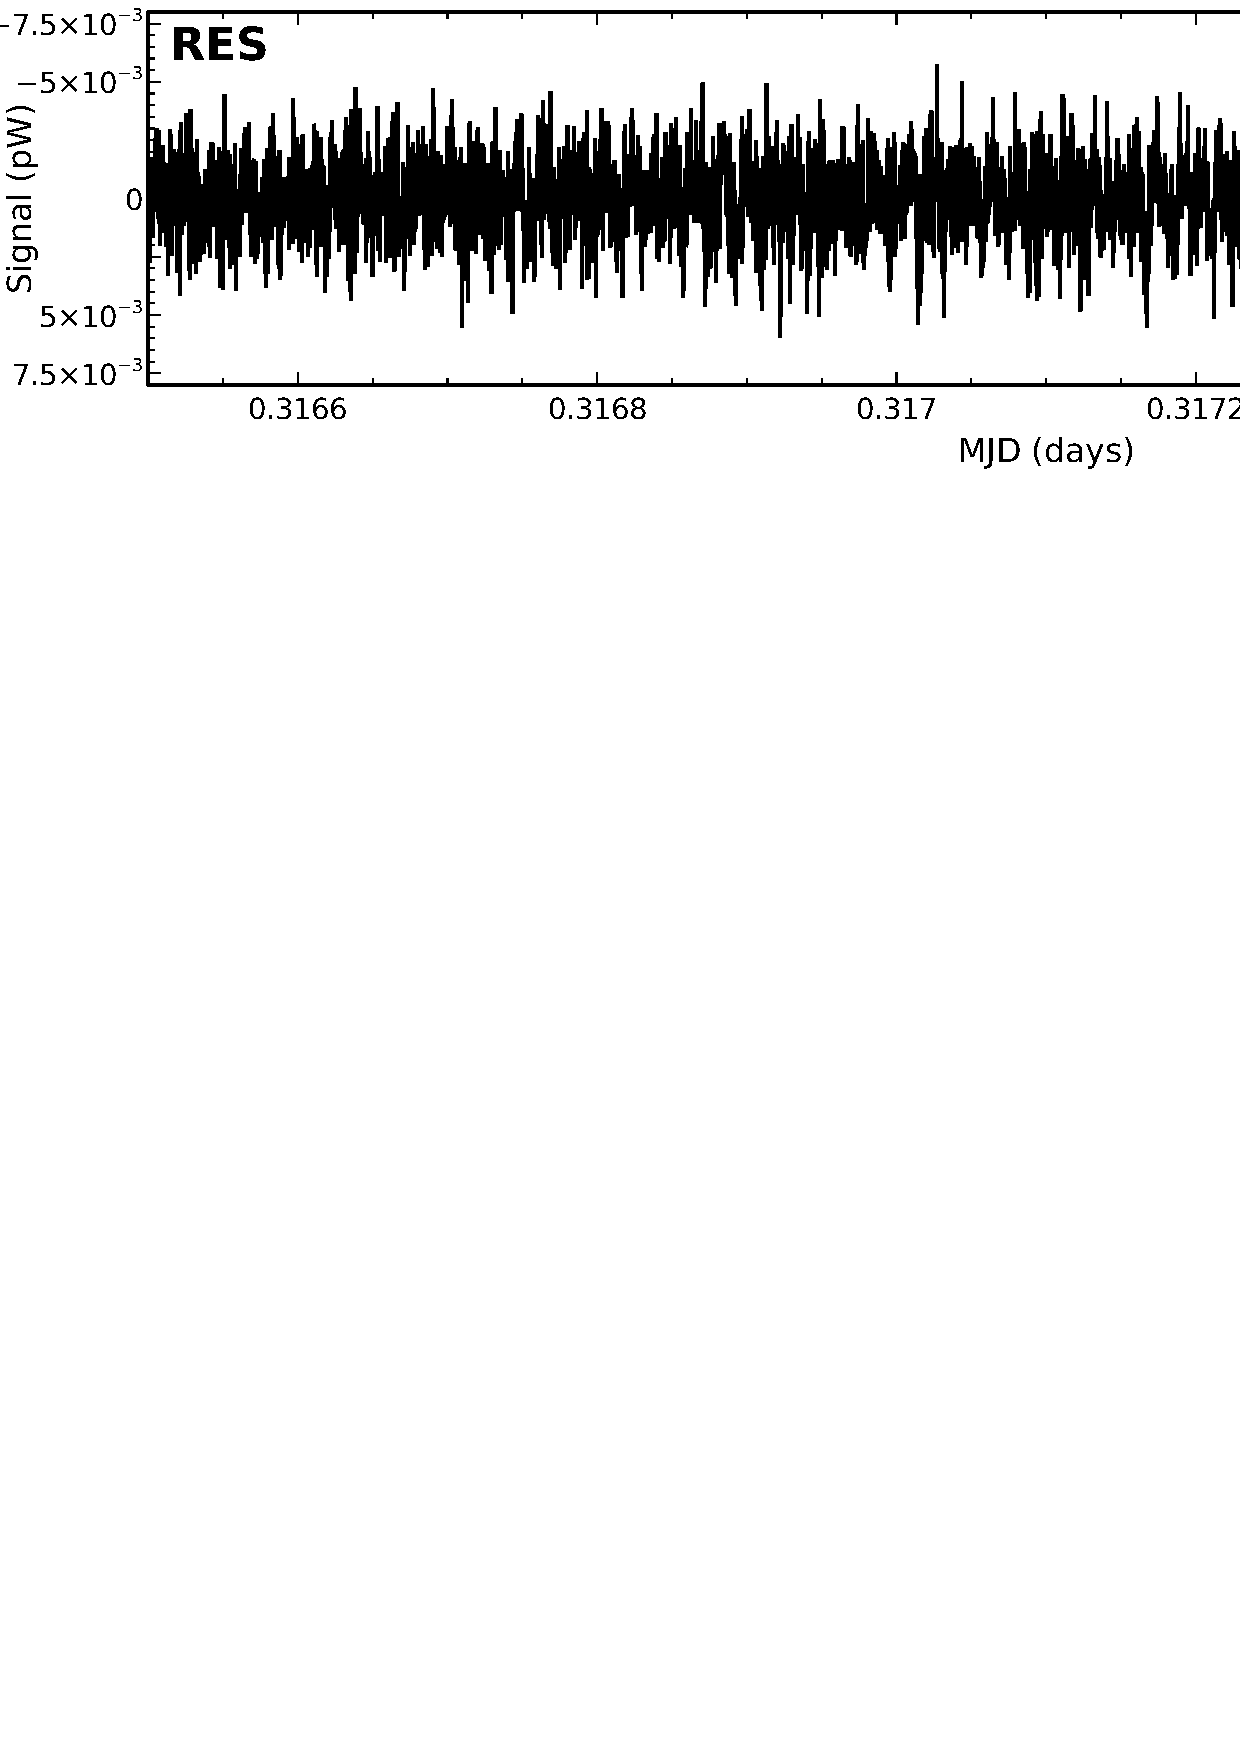
\includegraphics[width=\linewidth]{sc21_res} \\
\caption{\small Time-domain components of the iterative models. These
show the solution for the same single bolometer for part of an
observation of CRL2688. From top to bottom: the \texttt{COM} model
containing signal common to all bolometers, the \texttt{FLT} model
containing residual low-frequency noise missed by \texttt{COM}, the
\texttt{AST} model with the signal showing as a positive spike when
this bolometer passes over the source, and the \texttt{RES} model
looking (as expected) like white noise.}
\label{fig:itercomp}
\end{center}
\end{figure}
\end{latexonly}

By default, the final values of these fitted models are {\em not}
written out to files. However, this can be changed by setting
\texttt{exportndf} in the configuration file to the list of models
that you wish to view.

You can specify an additional component, \texttt{RES}, if you wish to
export the residual model. \texttt{RES} is the residual signal
remaining after the other models have been removed. By contrast, the
\texttt{NOI} model is the noise in \texttt{RES}, as determined by
running \texttt{RES} through \calcnoise\ (see
\cref{Section}{sec:calcnoise}{Checking the array performance}). If
\texttt{NOI} is exported, it can be
viewed as the VARIANCE component of the \texttt{RES} model; thus,
export of \texttt{RES} is implied if \texttt{NOI} is specified.

\vspace{0cm}
\begin{myquote}
\begin{verbatim}
exportndf = (com,gai,ast,flt,res,noi,qua)
\end{verbatim}
\end{myquote}
\vspace{0cm}
The \texttt{exportndf} parameter will write out the requested models
as NDF files with names based on the first input file that went into
the maps for each sub-array. This is first suffixed by \texttt{con},
indicating that several data files may have been concatenated
together. The three-letter code for each model is then appended to the
filename (such as \texttt{s8a20120720\_00030\_0003\_con\_com.sdf},
\begin{latexonly}
\linebreak          % \latex causes a paragraph break.
\end{latexonly}
\texttt{s8a20120720\_00030\_0003\_con\_flt.sdf},
\texttt{s8a20120720\_00030\_0003\_con\_res.sdf})\footnote{The filename shows
sub-scan 3 of Observation 30 since this is the first science file that
is encountered (see \cref{Section}{sec:raw}{Raw SCUBA-2 Data}).} The variance
and quality for the data are stored as the VARIANCE and QUALITY
components within the residual file NDF.

As with the input data, these are all standard {\starlink} NDF files
which can be examined using all of the existing Starlink tools.

Examples of the time traces for a single bolometer from these output
models are shown in \cref{Figure}{fig:itercomp}{time-domain components}.
These traces cover a
subset of an observation of the secondary calibrator CRL2688. The
\texttt{COM} model is removed first, being the dominant source. The
\texttt{FLT} model stores the data removed by the high-pass filter. In
the \texttt{AST} model, CRL2688 is clearly seen as positive spikes
which appear when the bolometer passes over the source. Finally, the
residual signal stored in \texttt{RES} is flat, indicating that most
of the signal has been successfully accounted for by the other model
components.

\begin{htmlonly}
\begin{figure}[h!]
\begin{center}
  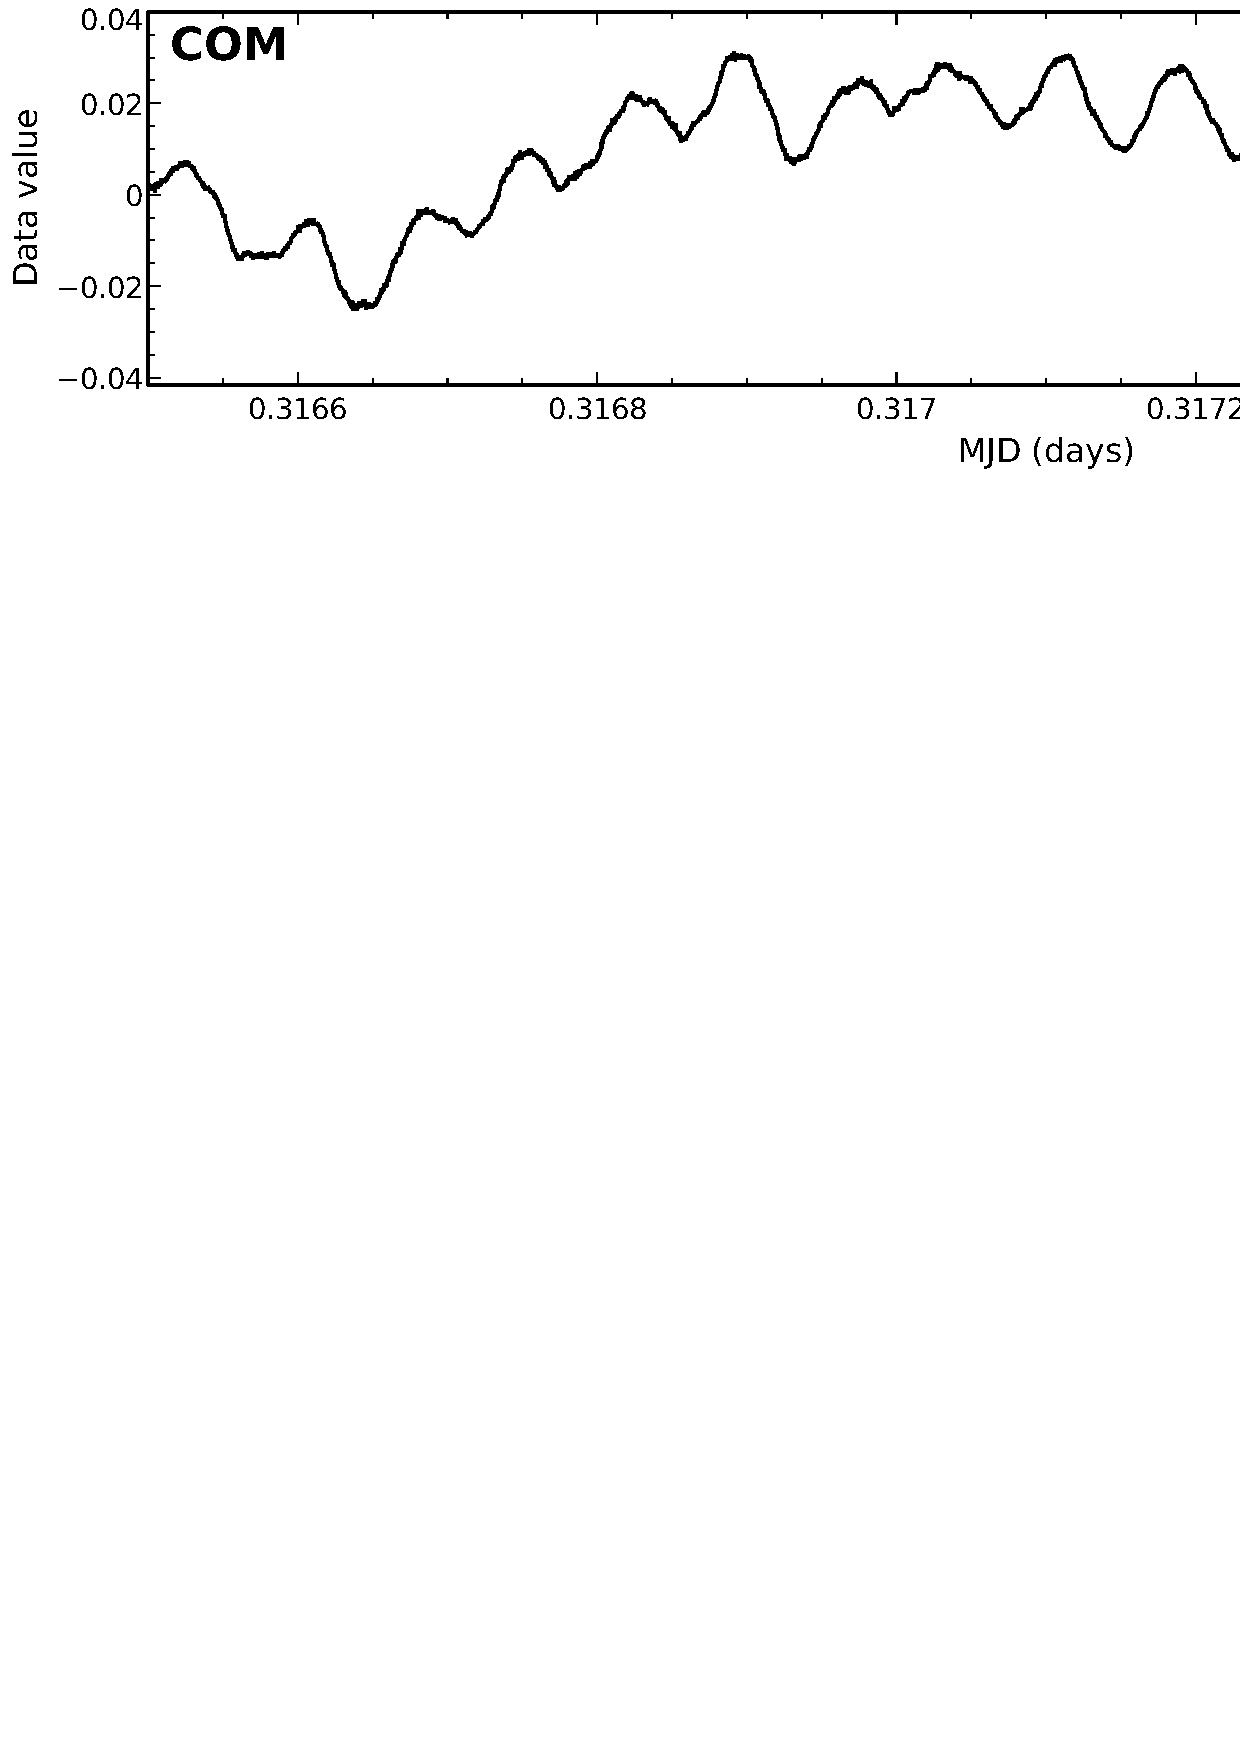
\includegraphics[width=136mm]{sc21_com} \\
  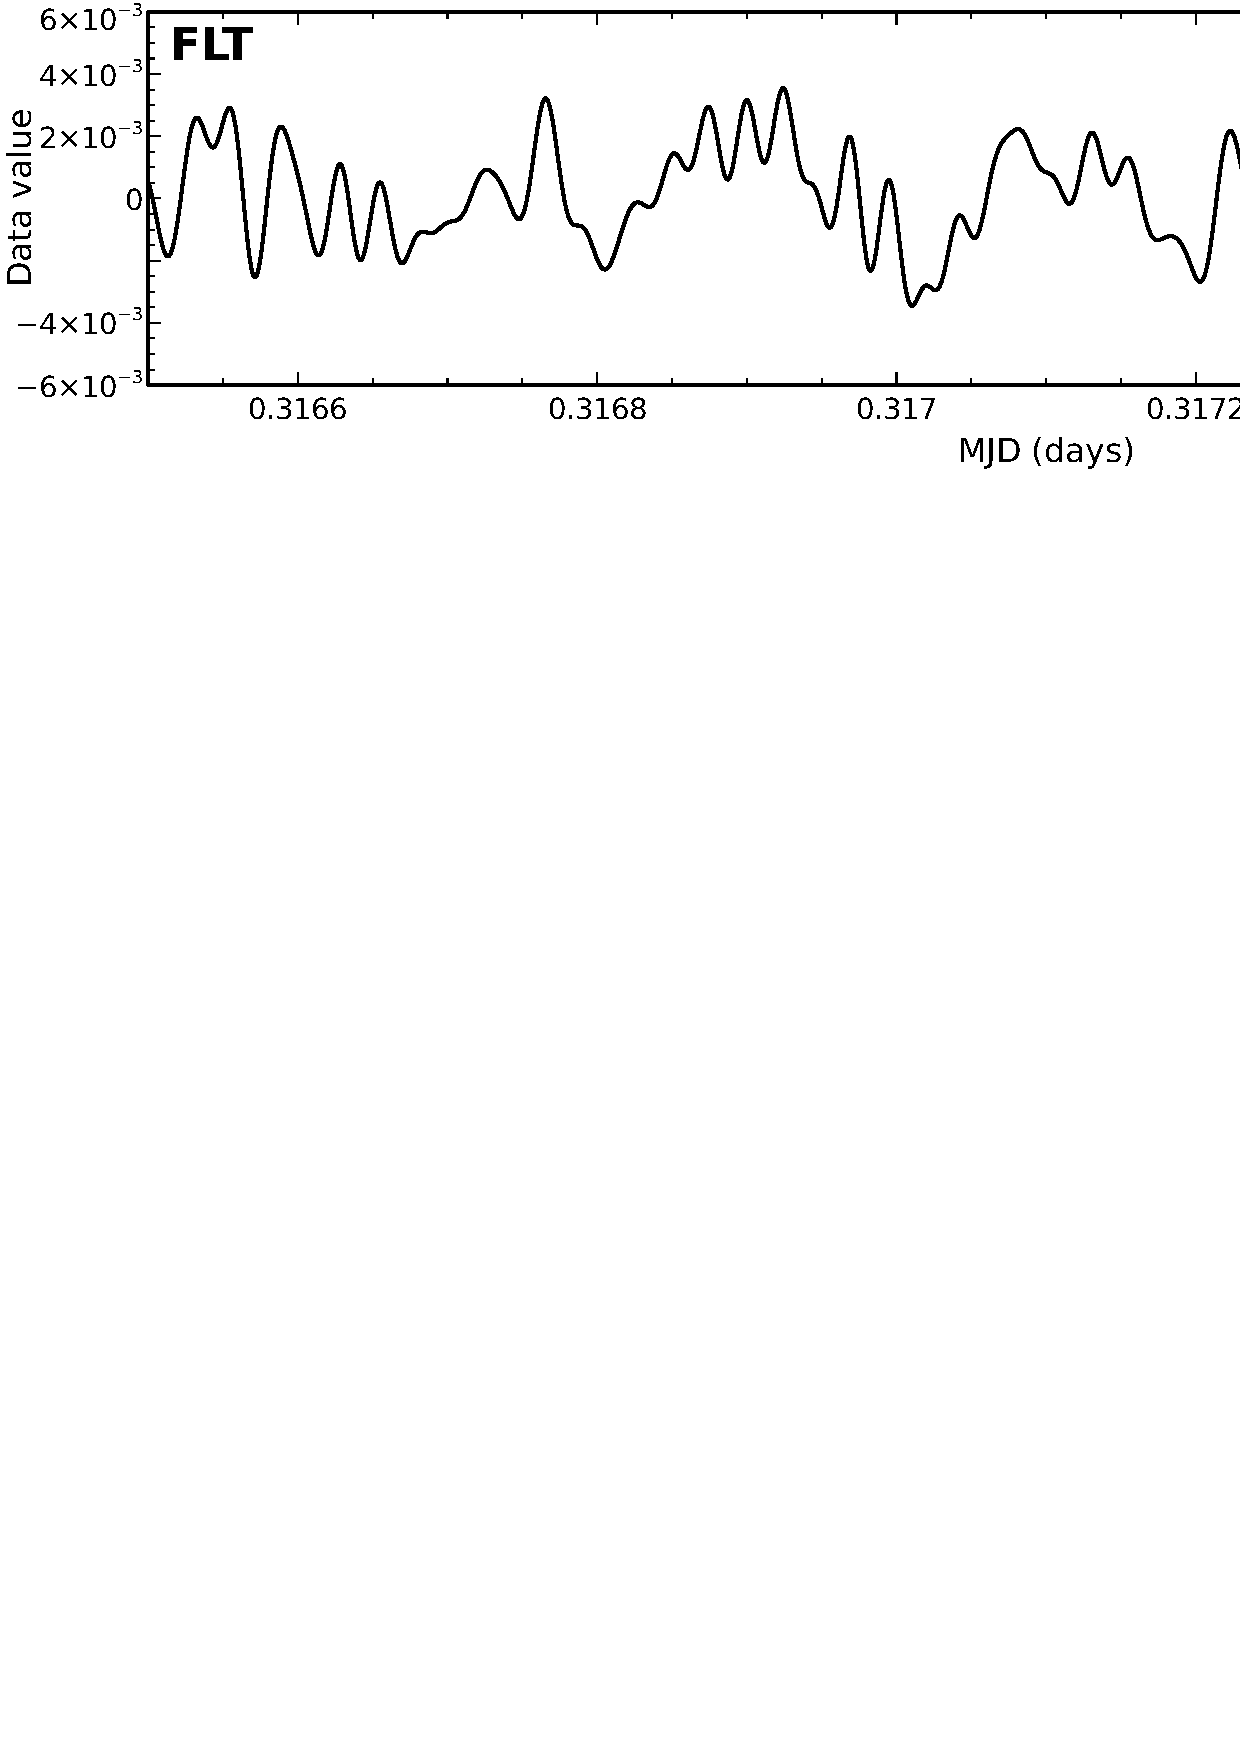
\includegraphics[width=136mm]{sc21_flt} \\
  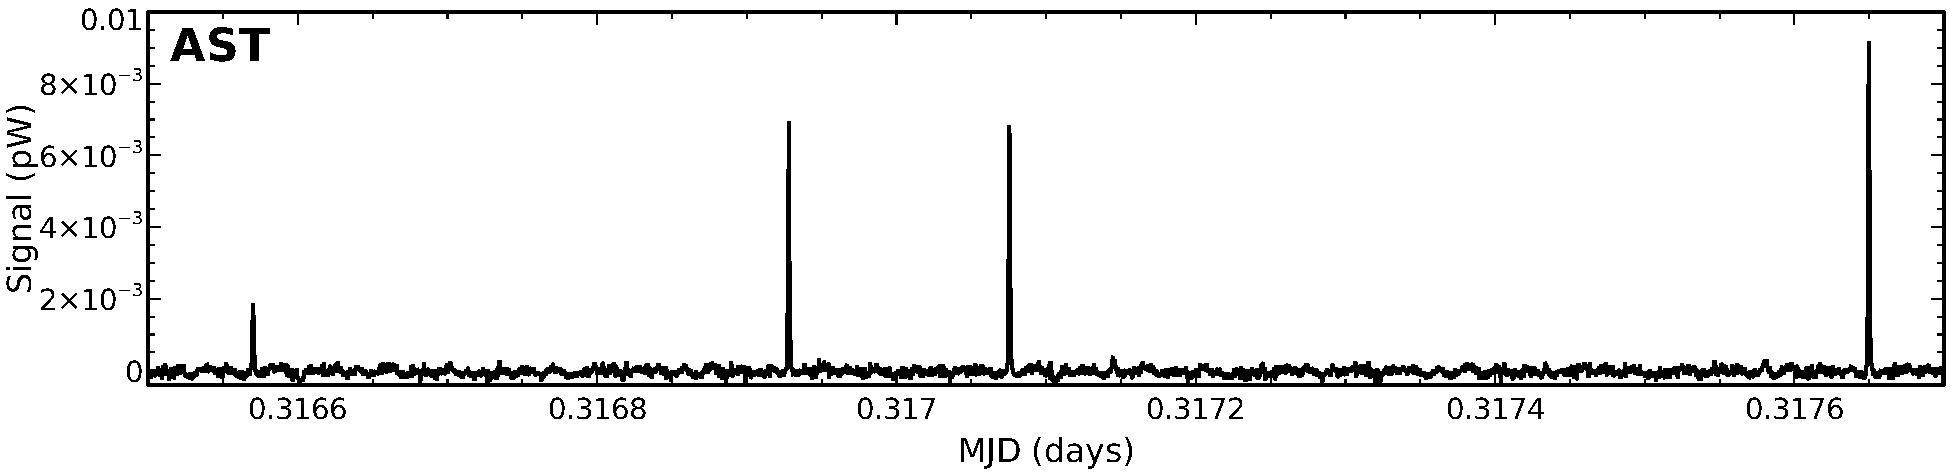
\includegraphics[width=136mm]{sc21_ast} \\
  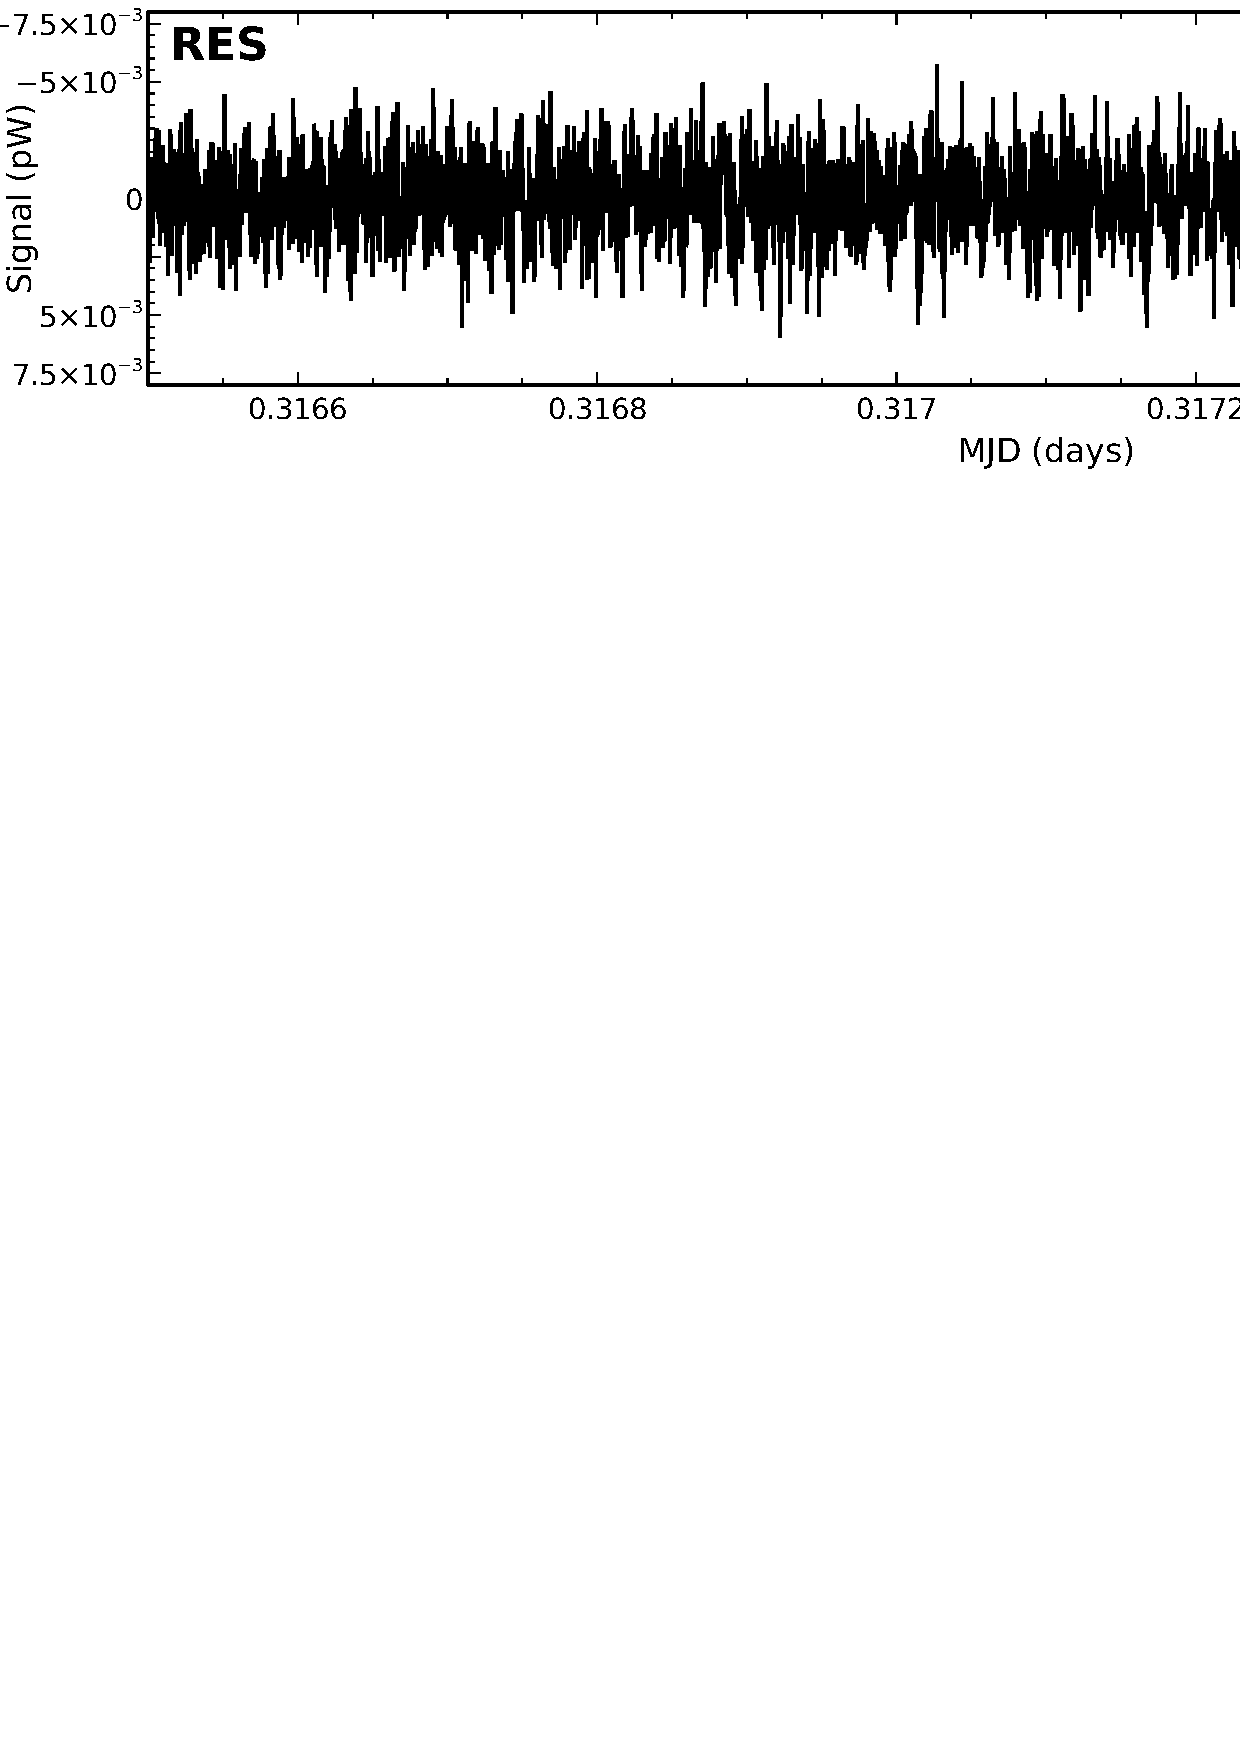
\includegraphics[width=136mm]{sc21_res} \\
\caption{\small Time-domain components of the iterative models. These
show the solution for the same single bolometer for part of an
observation of CRL2688. From top to bottom: the \texttt{COM} model
containing signal common to all bolometers, the \texttt{FLT} model
containing residual low-frequency noise missed by \texttt{COM}, the
\texttt{AST} model with the signal showing as a positive spike when
this bolometer passes over the source, and the \texttt{RES} model
looking (as expected) like white noise.}
\label{fig:itercomp}
\end{center}
\end{figure}
\end{htmlonly}



\subsection{\xlabel{config}Specialised configuration files}
\label{sec:config}

The default configuration file \texttt{dimmconfig.lis} is intended to
provide a reasonably good map for all types of observational
strategies and goals and compromises have been made to reach that
balance.

Whilst \texttt{dimmconfig.lis} is always a good recipe to start with
for your first run through of \makemap\ you will want to follow this up
with a specialised recipe that will match your observation. A number
of these specialised configuration files are supplied with \smurf\ and
can be found in \texttt{\$STARLINK\_DIR/share/smurf/} with file names
of the form \texttt{dimmconfig*.lis}. We suggest that you initially
run the map-maker with the default configuration file before trying
the configuration file relevant to your project.
\\ \\
The specialised files are all based on \texttt{dimmconfig.lis}, and
any parameters in these files simply override the relevant default
values. \cref{Table}{tab:dimmdef}{A table} lists all the active variables
contained in \texttt{dimmconfig.lis} and gives their default values
and a brief description. For comprehensive documentation on \emph{all}
available variables see the \texttt{dimmconfig.lis} file itself in
\cref{Appendix}{app:par_full}{an appendix}.
\\ \\
Below is a description of each of the specialised configuration files
available; the table following each description lists the parameters
set for each recipe. A verbatim copy of these files can be found in
\cref{Appendix}{app:special}{Specialised Configuration Files}.
\vspace*{3mm}
%
\myfig{sc21_dimmconfig4}{[t!]}{width=0.99\linewidth}{fig:inherit}{
  The inheritance order for the standard configuration files. Any
  parameters in the specialised configuration files override those in
  \texttt{dimmconfig.lis} which in turn override
  \texttt{smurf\_makemap.def}. If you chose to define your own
  parameter file you must specify its inheritance file.}

%

%
\subsubsection{dimmconfig\_blank\_field.lis}

This configuration is tuned for blank field surveys for which the goal
is to detect low signal-to-noise point sources. Blank field recipe
should be used for any map where the source is too faint to show up in
a 30-second scan.

Iteratively applying a high-pass
filter (\texttt{FLT}) can result in convergence problems when there is
little or no signal in the map; instead, a single, harsher high-pass
filter is applied as a pre-processing step (corresponding to
200-arcsec scales at both 450\,$\mu$m and 850\,$\mu$m). There are also
more conservative cuts to remove noisy/problematic bolometers. Only 4
(positive) iterations are requested as there is no signal to confuse
to models.

One of the options available in the map-maker allows the fitting of a
\texttt{COM} model to each sub-array separately. This option is
activated by setting \texttt{com.perarray = 1}. The model fit is
improved but with the loss of any structure on scales larger than a
single sub-array---not an issue for blank fields.

\cref{Figure}{fig:bfcompare}{The images below} shows the sharp
contrast in the output map between reducing data with the default
configuration file and using \texttt{dimmconfig\_blank\_field.lis}.

Normally blank-field maps would be subject to considerable
post-processing analysis (such as a jack-knife analysis and applying a
matched filter). All of these additional steps are outlined in
\cref{Section}{sec:cosmology}{Cosmology example}.
\vspace{0.3cm}
%
% The tildes around the equal sign are to ensure HTML table field is
% not wrapped after the parameter name.
\latex{\renewcommand*\arraystretch{0.8}}
\begin{table}[h!]
\centering
\begin{tabular}{|p{6.5cm}p{7.0cm}|}
\hline
\multicolumn{2}{|l|}{\texttt{dimmconfig\_blank\_field.lis}}\\
\hline
\texttt{numiter~=~4}&\texttt{flt\_edge\_largescale~=~200}\\
\texttt{spikethresh~=~10}&\texttt{model order~=~(com,ext,ast,noi)}\\
\texttt{com.perarray~=~1}&\\
\hline
\end{tabular}
\end{table}
%
\myfigduo{sc21_cosmo1-def}{sc21_cosmo1-bf}{[t!]}{width=0.47\linewidth}{fig:bfcompare}{3mm}{
 Maps of a deep cosmology field reduced with \textbf{(left)}
  \texttt{dimmconfig.lis} and \textbf{(right)} \texttt{dimmconfig\_blank\_field.lis}.}

\subsubsection{dimmconfig\_bright\_compact.lis}

This configuration is aimed at reducing maps of bright, compact
sources that are isolated at the centre of the map. It references
\texttt{dimmconfig\_bright.lis} (which in turn references
\texttt{dimmconfig.lis}), and thus the parameters from both `bright'
recipes override the default values in \texttt{dimmconfig.lis}.

The addition of \texttt{ast.zero\_circle} and
\texttt{ast.zero\_notlast} parameters are used to constrain the map to
zero beyond a radius of 1\,arcmin for all but the final iteration.
This strategy helps with map convergence significantly, and can
provide good maps of bright sources, even in cases where scan patterns
failed and the telescope degenerated into scanning back-and-forth
along a single position angle on the sky.

\texttt{com.perarray} is set to 1 indicating that a \texttt{COM} model
should be fit separately for each sub-array. This is not advised for
extended sources as signal on scales larger than a single sub-array is
lost but is fine for a compact central source. Likewise, the filtering
is tighter. The SNR threshold for DC steps is relaxed from 25 in the
default file to 100 to avoid problems associated with bright sources.

This is the recipe that is commonly used to reduce calibration
observations with a pixel size set to 1\,arcsec---see
\cref{Appendix}{app:fcf}{Flux conversion factors} for details on
determining the FCFs from calibrators.
\vspace{0.3cm}
%
%% The tildes around the equal sign are to ensure HTML table field is
%% not wrapped after the parameter name.
\latex{\renewcommand*\arraystretch{0.7}}
\begin{table}[h!]
\centering
\begin{tabular}{|p{6.5cm}p{7.0cm}|}
\hline
\multicolumn{2}{|l|}{\texttt{dimmconfig\_bright\_compact.lis}}\\
\hline
\texttt{numiter~=~-40}&\texttt{com.perarray~=~1}\\
\texttt{flt.filt\_edge\_largescale~=~200}& \texttt{flt.zero\_circle~=~(0.016666)}\\
 \texttt{ast.zero\_circle~=~(0.0166666666)}& \\
\hline
\multicolumn{2}{|l|}{\texttt{dimmconfig\_bright.lis}}\\
\hline
\texttt{noisecliphigh~=~10.0} & \texttt{dcthresh~=~100}\\
\texttt{com.corr\_tol~=~7}& \texttt{com.gain\_tol~=~7}\\
\texttt{com.gain\_abstol~=~5}& \\
\hline
\end{tabular}
\end{table}
%
\subsubsection{dimmconfig\_bright\_extended.lis}

This configuration is for reducing maps of bright extended sources.
The filtering is increased at 850\,$\mu$m to 600\,arcsec (600\,arcsec
is the default at 450\,$\mu$m), to aid the recovery of extended
emission.

Masking is used in this recipe where \texttt{ast.zero\_snr} is used to
constrain the \texttt{AST} model to zero wherever the SNR is lower
than 5$\,\sigma$. Everywhere the signal is below this threshold, the
\texttt{AST} model is set to zero for all but the final iteration
(\texttt{ast.zero\_notlast} is set to 1 in the default file). This
prevents ringing around bright sources. \texttt{numiter} has been
raised to \texttt{-40}, as more iterations are required to maximise
the sensitivity to large dynamic signal ranges in the map.

Recovering both faint extended structure and bright sources in the
same field poses an extra challenge. There are a number of options
available which build on the default recipe. The simplest is to set
the configuration parameter \texttt{ast.zero\_snrlo} which allows the
mask to grow organically as the \texttt{AST} model evolves. A second
is to supply an external mask; the simplest implementation of this is
to make your map using \texttt{dimmconfig\_bright\_extended.lis} then
generate a mask from the result, alternatively you can use a mask
generated from another dataset (e.g. Herschel). Instructions on
passing an external mask to the map-maker are outlined in
\cref{Section}{sec:maskbe}{Supplying an external mask}.
%
\cref{Figure}{fig:becompare}{The images below} shows a comparison
between maps reduced with the default configuration file and using
\texttt{dimmconfig\_bright\_extended.lis}; the most noticeable
difference is the improvement in the bowling around strong sources.
%
\latex{\renewcommand*\arraystretch{0.7}}
\begin{table}[h!]
\centering
\begin{tabular}{|p{6.5cm}|}
\hline
\texttt{dimmconfig\_bright\_extended.lis}\\
\hline
\texttt{numiter~=~-40}\\
\texttt{ast.zero\_snr~=~5}\\
\texttt{flt.filt\_edge\_largescale~=~600} \\
\hline
\end{tabular}
\end{table}

\myfigduo{sc21_gal_def_new}{sc21_gal_brex_new}{[h!]}{width=0.47\linewidth}{fig:becompare}{3mm}{
  A region towards the Galactic centre reduced with \textbf{(left)}
  \texttt{dimmconfig.lis} and \textbf{(right)} \texttt{dimmconfig\_bright\_extended.lis}.}
\latex{\renewcommand*\arraystretch{0.8}}
\clearpage
%
\section{\xlabel{maps}Reducing your Data}
\label{sec:maps}

This chapter describes how to run the map-maker and what to look out
for during processing. We also discuss reducing your data using the
\oracdr\ science pipeline and why you might want to chose this option.


\subsection{\xlabel{manual}Running the map-maker}

In the following example we produce a map of CRL2688, one of SCUBA-2's
secondary calibrators. As discussed in \cref{Section}{sec:dimm}{The
Dynamic Iterative Map-Maker}, all of the settings for the map-maker
are stored in configuration files. In this example we will just use
the default configuration file, \texttt{dimmconfig.lis}. For an
overview of the specialised configuration files available see
\cref{Section}{sec:config}{this section}.

As an input to the map-maker, any of the standard \smurf\
configuration files can be called directly from the Starlink path
with \texttt{\^\,\$STARLINK\_DIR/share/smurf/dimmconfig*.lis}.
Alternatively, a local copy can be made and called with
\texttt{\^\,dimmconfig*.lis}. Details of how to edit any of the
parameters can be found in \cref{Section}{sec:tweak}{Tweaking the
configuration file}.

A number of ADAM parameters are used by \makemap\ of which the
most important are: in, out, config, pixsize, ref, maxmem and
msg\_filter. Some of these appear in the example below but see
\cref{Appendix}{app:adam}{MAKEMAP ADAM Parameters} for the descriptions. A
complete list of all ADAM parameters can be found in \smurfsun.

\textbf{Note:} An up-caret (\,\^\,) is required any time you are reading in
a text file in \starlink. For the map-maker this includes the
configuration file and reading in a list of files as the input (e.g.
\texttt{in=\^\,rawfilelist.txt}).

The example uses \textbf{the
default pixel sizes which are 2\,arcsec for 450\,$\mu$m and 4\,arcsec for
850\,$\mu$m}. This can be overwritten by adding \texttt{pixsize=}$x$ to the
command string\footnote{The default sizes are defined as one quarter
of the Airy disk rounded up to the nearest half arcsecond.}, where $x$
is your desired pixel size in arcseconds. We advise that you do not
increase the pixel size at this stage as it will compromise model
fitting---instead regrid your map as a post-processing step.

Note that \texttt{method = iterate} has not been specified when
calling the map-maker as this this the default option.

\begin{myquote}
\begin{verbatim}
% makemap in='/jcmtdata/raw/scuba2/s8*/20120720/00030/*.sdf' out=850_crl2688\
  config=^$STARLINK_DIR/share/smurf/dimmconfig.lis


Out of 32 input files, 4 were darks, 8 were fast flats and 20 were science
Processing data from instrument 'SCUBA-2' for object 'CRL2688' from the
following observation :
20120720 #30 scan /shutter

MAKEMAP: Map-maker will use no more than 68401 MiB of memory

Projection parameters used:
CRPIX1 = 0
CRPIX2 = 0
CRVAL1 = 315.578333333333 ( RA = 21:02:18.800 )
CRVAL2 = 36.6938055555556 ( Dec = 36:41:37.70 )
CDELT1 = -0.00111111111111111 ( -4 arcsec )
CDELT2 = 0.00111111111111111 ( 4 arcsec )
CROTA2 = 0

Output map pixel bounds: ( -132:122, -126:129 )

Output map WCS bounds:
Right ascension: 21:01:38.318 -> 21:03:03.280
Declination: 36:33:07.19 -> 36:50:11.70

smf_iteratemap: will down-sample data to match angular scale of 4 arcsec
smf_iteratemap: Iterate to convergence (max 5)
smf_iteratemap: stop when change in chi^2 < 0.001
smf_iteratemap: provided data are in 1 continuous chunks, the largest of which
has 5957 samples (153.729 s)
smf_iteratemap: map-making requires 1376 MiB (map=3 MiB model calc=1372 MiB)
smf_iteratemap: Continuous chunk 1 / 1 =========
smf_calc_smoothedwvm: 0.977444 s to calculate unsmoothed WVM tau values
smf_iteratemap: Iteration 1 / 5 ---------------
--- Size of the entire data array ------------------------------------------
bolos : 5120
tslices: bnd:0(0.0 min), map:5957(2.6 min), tot:5957(2.6 min)
Total samples: 30499840
--- Quality flagging statistics --------------------------------------------
 BADDA:   10972794 (35.98%),        1842 bolos
BADBOL:   11818688 (38.75%),        1984 bolos
DCJUMP:      38809 ( 0.13%),
  STAT:      71680 ( 0.24%),          14 tslices
 NOISE:     810152 ( 2.66%),         136 bolos
Total samples available for map:   18634826, 61.10% of max (3128.22 bolos)
smf_iteratemap: Calculate time-stream model components
smf_iteratemap: Rebin residual to estimate MAP
smf_iteratemap: Calculate ast
--- Quality flagging statistics --------------------------------------------
 BADDA:   10972794 (35.98%),        1842 bolos  ,change          0 (+0.00%)
BADBOL:   11925914 (39.10%),        2002 bolos  ,change     107226 (+0.91%)
DCJUMP:      38809 ( 0.13%),                    ,change          0 (+0.00%)
  STAT:      71680 ( 0.24%),          14 tslices,change          0 (+0.00%)
   COM:     323165 ( 1.06%),                    ,change     323165 (+0.00%)
 NOISE:     810152 ( 2.66%),         136 bolos  ,change          0 (+0.00%)
Total samples available for map:   18312771, 60.04% of max (3074.16 bolos)
     Change from last report:    -322055, -1.73% of previous
smf_iteratemap: Will calculate chi^2 next iteration
smf_iteratemap: *** NORMALIZED MAP CHANGE: 0.874979 (mean) 73.7106 (max)
smf_iteratemap: Iteration 2 / 5 ---------------
smf_iteratemap: Calculate time-stream model components
smf_iteratemap: Rebin residual to estimate MAP
smf_iteratemap: Calculate ast
--- Quality flagging statistics --------------------------------------------
 BADDA:   10972794 (35.98%),        1842 bolos  ,change          0 (+0.00%)
BADBOL:   11949742 (39.18%),        2006 bolos  ,change      23828 (+0.20%)
 SPIKE:         34 ( 0.00%),                    ,change         34 (+0.00%)
DCJUMP:      38809 ( 0.13%),                    ,change          0 (+0.00%)
  STAT:      71680 ( 0.24%),          14 tslices,change          0 (+0.00%)
   COM:     357816 ( 1.17%),                    ,change      34651 (+10.72%)
 NOISE:     810152 ( 2.66%),         136 bolos  ,change          0 (+0.00%)
Total samples available for map:   18278374, 59.93% of max (3068.39 bolos)
     Change from last report:     -34397, -0.19% of previous
smf_iteratemap: *** CHISQUARED = 0.983228126551834
smf_iteratemap: *** NORMALIZED MAP CHANGE: 1.29181 (mean) 15.0552 (max)
smf_iteratemap: Iteration 3 / 5 ---------------
.....
.....
.....
smf_iteratemap: Iteration 5 / 5 ---------------
smf_iteratemap: Calculate time-stream model components
smf_iteratemap: Rebin residual to estimate MAP
smf_iteratemap: Calculate ast
--- Quality flagging statistics --------------------------------------------
 BADDA:   10972794 (35.98%),        1842 bolos  ,change          0 (+0.00%)
BADBOL:   11949742 (39.18%),        2006 bolos  ,change          0 (+0.00%)
 SPIKE:         34 ( 0.00%),                    ,change          0 (+0.00%)
DCJUMP:      38809 ( 0.13%),                    ,change          0 (+0.00%)
  STAT:      71680 ( 0.24%),          14 tslices,change          0 (+0.00%)
   COM:     362902 ( 1.19%),                    ,change          0 (+0.00%)
 NOISE:     810152 ( 2.66%),         136 bolos  ,change          0 (+0.00%)
Total samples available for map:   18273302, 59.91% of max (3067.53 bolos)
     Change from last report:          0, +0.00% of previous
smf_iteratemap: *** CHISQUARED = 0.952708604771402
smf_iteratemap: *** change: -0.000109049487216351
smf_iteratemap: *** NORMALIZED MAP CHANGE: 0.107427 (mean) 2.96138 (max)
smf_iteratemap: ****** Completed in 5 iterations
smf_iteratemap: ****** Solution CONVERGED
Total samples available from all chunks: 18273302 (3067.53 bolos)
\end{verbatim}
\end{myquote}
\vspace{-10mm}
\begin{center}
\latex{\line(1,0){155}}
\end{center}

\subsection{\xlabel{look_for}What to look out for}
%\flushbottom

Once the map-maker has completed you can open your output map using
\gaia---see \cref{Figure}{fig:itermap}{the figure below}. The excerpt
above shows the output written to the terminal as you run the map-maker. There
are a number of clues in this output that indicate the status of the
reduction.


\textbf{The number of input files}\\
The first to note is the number of input files; it is worth checking
this matches your expected number. Also summarised are the source
name, UT date and scan number.
\\ \\
\textbf{Map dimensions}\\
Next the basic dimensions of the data being processed are listed near
the start of the first iteration. The example above has 4\,arcsec pixels
-- the default at 850\,$\mu$m.
\\ \\
\textbf{Chunking}\\
\label{box:chunk}
The map-maker then determines if the raw data should be split and
processed in more than one chunk. In this map the data is reduced in
one continuous piece: \param{Continuous chunk 1 / 1}. Chunking is
where the map-maker processes sub sections of the time-series data
independently and should be avoided if possible---see the text box
\begin{latexonly}
on Page~\pageref{page:text}.
\end{latexonly}
\begin{htmlonly}
below.
\end{htmlonly}
\\

% The minipages used for the dvi version give latex2html problems.
\begin{htmlonly}
\htmladdimg{sc21_data_chunking.png}
\\ \\
\end{htmlonly}

\myfig{sc21_crl2688}{[t!]}{width=0.7\linewidth}{fig:itermap}{
Map of CRL2688 produced with the \smurf\ task \makemap\ using
the iterative algorithm with default parameters.}

\textbf{Quality statistics}\\
Next come the QUALITY flagging statistics. At the beginning, the main
purpose is to indicate how many bolometers are being used. In the
example above you can see that from a total of 5120 bolometers, 1842
were turned off during data acquisition (\texttt{BADDA}). In addition,
136 bolometers exceeded the acceptable noise threshold
(\texttt{NOISE}), while tiny fractions of the data were flagged
because the telescope was moving too slowly (\texttt{STAT}) or the
sample are adjacent to a step that was removed (\texttt{DCJUMP}).

The total number of bad bolometers (\texttt{BADBOL}) is 1984.
Accounting for these, and the small numbers of additionally flagged
samples, 3128.22 effective bolometers are available after initial
cleaning\footnote{The fractional number is due to time-slices being
removed during cleaning. The number of bolometers is then
reconstructed from the number of remaining time-slices}.


After each subsequent iteration a new `Quality' report is produced,
indicating how the flags have changed. An important flag that appears
in the `Quality' report following the first iteration is \texttt{COM}:
the DIMM rejects bolometers (or portions of their time series) if they
differ significantly from the common-mode (average) of the remaining
bolometers.

You may note that compared with the initial report, the total number of samples
with good `Quality' (\texttt{Total samples available for map}) has
dropped from 18634826 to 18273302 (about a 2 per cent decrease) as
additional samples were flagged in each iteration.


\begin{latexonly}
\begin{center}
\begin{fmpage}{0.92\linewidth}
\label{page:text}
\begin{minipage}[t!]{0.025\linewidth}
\hspace{0.1cm}
\end{minipage}
\begin{minipage}[t!]{0.93\linewidth}
\vspace{0.2cm}
\textbf{Data Chunking}\\
Chunking occurs when there is insufficient computer memory available
for the map-maker or when there is a gap in the time-series data (e.g.
from a missing sub-scan). In these cases, the map-maker divides up the
time-series and reduces each sub-portion independently, producing a
separate map for each, before finally coadding all the maps at the
end. Ideally you want your data reduced in a single chunk, however
this can be unfeasible for large maps.
\vspace{0.2cm}\\
The more data the map-maker processes at once, the better chance it
has of determining the difference between sky signal and background
noise. In \textsc{daisy} mode chunking is less of a concern as
the entire map area is covered many times in the space of a single
observation.
\vspace{0.2cm}\\
For \textsc{pong} maps chunking is a bigger concern, with the
maximum number of chunks that can be tolerated dependent on the number
of map rotations. For example, a 40-minute \textsc{pong} map with 8
rotations may get divided into three or four chunks. Although not
ideal, this will mean that each point is still covered by two or three
passes. Fewer passes than this however and the map-maker become less
effective.
\vspace{0.2cm}
\end{minipage}
\begin{minipage}[t!]{0.025\linewidth}
\hspace{0.1cm}
\end{minipage}
\end{fmpage}
\end{center}
\end{latexonly}

Be aware that some large reductions may take many iterations to reach
convergence and you may find significantly fewer bolometers remaining
resulting in higher noise than expected.
\\ \\
\textbf{Convergence}\\
What about the convergence parameter? As discussed in
\cref{Section}{sec:converge}{Convergence} there are two noise based
convergence criteria that can be set---\texttt{maptol} and \texttt{chitol}.

Both are reported during processing but only one will be used to determine
if convergence has been achieved.
\\
Convergence based on \texttt{maptol} can be checked from the line
reporting\\
\hspace{5mm}\texttt{smf\_iteratemap: *** NORMALIZED MAP
CHANGE: 0.10559 (mean) 2.81081 (max)}.\\
In the line above the number to look out for is the mean value. This
will have to drop below your required \texttt{maptol} for successful
convergence.

\texttt{chitol} convergence can be monitored by the
\texttt{CHISQUARED} value---the RMS of the residual (time series with
the various model components removed) for all of the samples with good
`Quality', normalised by the measured white noise levels. This can be
seen in the line below.\\
\hspace{0.5cm}\texttt{smf\_iteratemap: *** CHISQUARED = 0.872127100064999}


The default configuration file used in this example executes a maximum
of 5 iterations, but stops sooner if the change in \texttt{CHISQUARED}
is less then 0.001 (i.e. \texttt{numiter=-5}). In this example it
stops after 5 iterations: \\
\texttt{smf\_iteratemap: *** Completed in 5 iterations}.


\textbf{Note:} you can interrupt the processing at any stage with a
single \texttt{Ctrl-C}. The map-maker will complete the iteration then write
out a final science map. If you enter \texttt{Ctrl-C} a second time it will
kill the process immediately.

\subsection{\xlabel{sciencepl}Using the science pipeline}

You can also reduce your data using the \oracdr\ science pipeline on a
local computer. There are advantages to running the map-maker using
the pipeline. You can feed the pipeline observations of multiple
sources rather than feed in a single source at a time. The pipeline
will recognise the different sources and make a separate map for each,
whereas the map-maker would make a single large map that would include
all your sources (no matter how widely spaced!). Another useful
feature is that the pipeline will generate a log files to record
various useful quantities. The standard log files from reducing
science data are:
\\*
\begin{itemize}
\item log.noise---noise in the map for each observation and the coadd
(calculated from median of error component)
\item log.nefd---NEFD calculated for each observation and for the coadded map(s)
\end{itemize}
The pipeline will produce calibrated maps; by default these are
calibrated using the standard FCFs, although users can specify their
own if they wish.

Running the science pipeline is very straightforward and can be as
simple as the example below. Here a list is made of all your raw data,
the pipeline is then initiated, finally the reduction is started with
instructions to loop through all data listed in the supplied file and
the filename in question is given.

\begin{myquote}
\begin{verbatim}
% ls s8*.sdf > myfiles.lis
% oracdr_scuba2_850
% oracdr -loop file -files myfiles.lis
\end{verbatim}
\end{myquote}

You should be aware that you can supply the JAC with a tailored
configuration file or more complicated data-reduction script that you
would like to be associated with your project. The project can be
re-reduced using this tailored recipe and data products reduced to
your specification will be made available at CADC. This is
particularly useful for very large survey-scale projects.

For a more in-depth discussion on running the pipeline and a discussion
of the various outputs see \cref{section}{sec:pipe}{The SCUBA-2
Pipeline} or \pipelinesun.
\clearpage

\section{\xlabel{maps}Post-processing Reduction Steps}
\label{sec:postprocess}

This chapter describes the steps you are likely to want to take after
the map-maker has produced a science map. These include calibrating
your data by applying an FCF, dealing with multiple maps, checking the
noise levels and cropping your map.
\\*\\*
The software used for these post-processing steps are \Kappa\ and
\picard. \picard\ is specially designed to operate on the map-maker
products (and hence also on pipeline products) and a number of tailored
recipes exist to make these steps easier to perform. We recommend you
consult the \picard\ manual (see \picardsun) for a full list of
available recipes. General \picard\ options can be accessed by typing
\texttt{picard -h} in a terminal.

\subsection{\xlabel{apply_fcf}Flux Conversion Factor (FCF)}
\label{sec:cmult}

When your data comes out of the map-maker it is unit of picowatts
(pW). A flux conversion factor, or FCF, needs to be applied to scale
your data from units of pW to Janskys. For more information on calibrating
SCUBA-2 data see Dempsey et al. (2013) \cite{dempsey12}.
\\*\\*
JAC provides default values for the various FCFs which have been proven
to be stable. These standard numbers are applied by the pipeline when
reducing your data with \oracdr. For reduction dates from July 2012
onwards the FCF factors are:
\begin{table}[h!]
\centering
\begin{tabular}{|c|c|c|c|}
\hline
\multicolumn{2}{|c|}{FCF$_{aperture}$ (Jy/pW/arcsec$^2$) } &
\multicolumn{2}{c|}{FCF$_{peak}$ (Jy/pW/beam)} \\
\hline
\hspace{0.4cm} 450\,$\mu$m \hspace{0.3cm} & 850\,$\mu$m & \hspace{0.4cm} 450\,$\mu$m \hspace{0.3cm}& 850\,$\mu$m \\
\hline
4.71 $\pm$ 0.5& 2.34 $\pm$ 0.08& 491 $\pm$ 67& 537 $\pm$ 24 \\
\hline
\end{tabular}
\end{table}
\\
\textbf{IMPORTANT NOTES: (1) The standard FCF to be applied depends on
the reduction date for your data. For data that have been
\emph{reduced prior} to July 2012 you should see
\cref{Appendix}{app:fcfs}{FCFs by Reduction Date} for alternative
FCFs. (2) Due to a glitch in the WVM, data reduced between Sept. 19,
2012 and Jan. 18, 2013 must be re-reduced using the latest version of
Starlink (Hikianalia or later), or should have an FCF derived from a
calibrator reduced at the same time (and not our standard FCF) applied
to it. }

\subsubsection{Peak FCF}

If you want to read off the \textbf{peak flux} from your map, you
should multiply your map by the \fcfb\ (also known as the peak FCF).
Thus, when you open your map in \gaia\ the value of the brightest
pixel will be the peak flux of your source. Applying \fcfb\ will
result in a map with units of Jy/beam. For point-like or compact
sources smaller than the beam (with a Gaussian profile), this peak
value will be the flux density of your source. Be aware that the
pipeline (see \cref{Section}{sec:pipe}{SCUBA-2 Pipeline}) reports FCFs
in units of mJy/beam.  Note that \fcfb\ applies to the default pixel
sizes (4\,arcsec at 850\,$\mu$m and 2\,arcsec at 450\,$\mu$m). For
pixel sizes other than these, \fcfb\ will need to be scaled accordingly.

\subsubsection{Aperture FCF}

To get the flux density of extended sources with \textbf{aperture
photometry} you should apply the \fcfa. You will also need to multiply
your map by the square of the pixel size (i.e. 16 for 4'' pixels).
Only then can you sum the emission in an aperture. \fcfa\ was
determined using a 60\,arcsec diameter aperture. If your aperture
differs from this you should scale your flux accordingly---the scaling
factor can be read off the curve of growth (see
\cref{Appendix}{app:cog}{Aperture Photometry Curve of Growth}). This
graph gives the ratio of aperture flux to total flux for a range of
aperture diameters.

\subsubsection{Determining your own FCF}

Calibration observations are taken at various points throughout the
night and we recommend you compare the FCF calculated from your
nearest calibrator to the standard FCF. You can use this FCF to scale
the the standard value accordingly. You should chose the calibrator
nearest in time to your science observations, unless the weather has
changed significantly.
\vspace{1mm}\\
\begin{minipage}[t]{0.05\linewidth}
\texttt{(1)}
\end{minipage}
\begin{minipage}[t]{0.95\linewidth}
 You should first reduce the calibrator with the map-maker using
 \texttt{dimmconfig\_bright\_compact.lis} as your configuration file.
\end{minipage}
\vspace{1mm}\\
\begin{minipage}[t]{0.05\linewidth}
\texttt{(2)}
\end{minipage}
\begin{minipage}[t]{0.95\linewidth}
Next determine the FCF value by passing the resulting map to the
\picard\ recipe \xref{\drrecipe{SCUBA2\_CHECK\_CAL}}{sun265}{SCUBA2_CHECK_CAL}.
\begin{myquote}
\begin{verbatim}
% picard SCUBA2_CHECK_CAL 850calibrator.sdf
\end{verbatim}
\end{myquote}
This will produce a log file (\texttt{log.checkcal}) which records the both
\fcfb\ and \fcfa. Check that these values closely approximate the
standard FCF values given above.
\end{minipage}
\vspace{1mm}\\
\begin{minipage}[t]{0.05\linewidth}
\texttt{(3)}
\end{minipage}
\begin{minipage}[t]{0.95\linewidth}
Re-reduce the calibrator using the map-maker with the \emph{same}
configuration file you used for your science observations. Once again
determine the FCF using \drrecipe{SCUBA2\_CHECK\_CAL}.
\end{minipage}
\vspace{1mm}\\
\begin{minipage}[t]{0.05\linewidth}
\texttt{(4)}
\end{minipage}
\begin{minipage}[t]{0.95\linewidth}
Apply this FCF to your reduced science data using \cmult. (Remember to
also apply the pixel size squared factor if using \fcfa.)
\end{minipage}

\subsubsection{Applying the FCF using \cmult}

You can multiply your data file by the FCF, or by any other constant
factor, using the \Kappa\ command \cmult. This application multiplies
each pixel in an NDF by a scalar to produce a new NDF. In the example
below the output map is in units of mJy/beam.

\begin{myquote}
\begin{verbatim}
% cmult in=850map.sdf out=850map_cal scalar=537000
\end{verbatim}
\end{myquote}


\subsection{\xlabel{coadd}Coadding multiple maps}
\label{sec:coadd}

You may have multiple maps of the same source which you would like to
coadd. \picard\ has a recipe called
\xref{\drrecipe{MOSAIC\_JCMT\_IMAGES}}{sun265}{MOSAIC_JCMT_IMAGES}
that coadds maps while correctly dealing with the exposure time and
weights NDF extensions.
\begin{myquote}
\begin{verbatim}
% picard -recpars mypar.lis MOSAIC_JCMT_IMAGES 850map*_cal_crop.sdf
\end{verbatim}
\end{myquote}
This creates a single output file based on the name of the last file
in the list, and with a suffix \texttt{\_mos}.

There are a number of options associated with
\param{MOSAIC\_JCMT\_IMAGES} (see the \textsc{Picard} manual for a full
description). However, the main one is choosing between \wcsmosaic\
(default) and the \ccdpack\ option \makemos\ for the combination
method. For more information on \task{makemos} and advice on choosing the
best method see \xref{SUN/139}{sun139}{}.

An example parameter file like the one below chooses \task{makemos}
using a 3-$\sigma$ clipping threshold.
\begin{myquote}
\begin{verbatim}
[MOSAIC_JCMT_IMAGES]
MOSAIC_TASK = makemos
MAKEMOS_METHOD = sigmas
MAKEMOS_SIGMAS = 3
\end{verbatim}
\end{myquote}
Another option available (either independently or within this recipe)
is to register the images. This can be used when there is a common,
known source that is present in \emph{all} of the input maps. The
position of that source can be given and the recipe
\xref{\drrecipe{SCUBA2\_REGISTER\_IMAGES}}{sun265}{SCUBA2_REGISTER_IMAGES}
fits a profile to the source and shifts the map accordingly so they
are all aligned.

\textbf{Note:} If you wish to give \picard\ an input list file you should
use the \texttt{cat} command with back quotes like so:
\begin{myquote}
\begin{verbatim}
% picard MOSAIC_JCMT_IMAGES `cat listoffiles.txt`
\end{verbatim}
\end{myquote}


Currently there is no advantage in terms of data quality to reducing
all observations simultaneously or separately. However, the latter
does allow the option of assessing the individual maps before coadding
and is the method followed in this example.

\subsection{\xlabel{crop}Cropping your map}
\label{sec:crop}

The nature of the scan patterns results in SCUBA-2 maps significantly
larger than the requested size. The high noise towards the outer edges
is a consequence of the scanning operation (i.e. the telescope moving
slowly as it reverses direction and reduced integration time) and
should not be included in your final map.

You can crop your map to the map size specified in the data header or
to any requested size of box or circle using the \picard\ command
\xref{\param{CROP\_JCMT\_IMAGES}}{sun265}{CROP_JCMT_IMAGES}. The centre
of the cropping area will always be the centre of your map.
\begin{myquote}
\begin{verbatim}
% picard -recpars mypar.lis CROP_JCMT_IMAGES 850map_cal.sdf
\end{verbatim}
\end{myquote}
The example above includes a parameter file specifying the radius of
the circle to be extracted (in arcsecs). The format for the parameter
file is shown below.
\begin{myquote}
\begin{verbatim}
[CROP_JCMT_IMAGES]
MAP_RADIUS = 1800.0
\end{verbatim}
\end{myquote}
If this parameter file is omitted it will default to a box of sides
equal to the map size in the header (as requested in the MSB). Be
aware that the circular nature of the scan patterns means that good
data will be lost if you chose a square or rectangular map.

The output from \drrecipe{CROP\_JCMT\_IMAGES} is a file with the suffix
\texttt{\_crop}. Full details of this recipe can be found in the
\htmladdnormallink{\textsc{Picard} manual}{http://www.oracdr.org/oracdr/PICARD}
\latex{\footnote{\texttt{http://www.oracdr.org/oracdr/PICARD}}}.

\subsection{\xlabel{noise}Calculating the noise}

These steps apply to the output from the map-maker---either as a
result of running it manually or using the reduced files downloaded
from the \htmladdnormallink{JCMT Science
Archive.}{http://www3.cadc-ccda.hia-iha.nrc-cnrc.gc.ca/jcmt/} One of
the first checks you can do is to open your map in \gaia\ and check
the flatness of the background. If it passes visual inspection you
will want to know what noise level you have reached.
\\ \\
If you have not already cropped your map you should do so. The data at
the edges of the map are considerably noisier due to reduced exposure
time, so to get an accurate RMS you will need to remove these noisy
edges---see \cref{Section}{sec:crop}{Cropping your map}.

Once cropped, the noise can then be read from the statistics of the
file. The \Kappa\ command \stats\ may be used for this:
\begin{myquote}
\begin{verbatim}
% stats comp=err order=true 850map_cal_crop
\end{verbatim}
\end{myquote}
The \param{comp=err} string specifies that the error component of the
file should be read, while \param{order=true} gives you the median.
\textbf{The `Pixel mean' and `Pixel median' values are then the mean
and median RMS for your science map in Jy.}

\textbf{Note:} If you do not use the \param{comp=err} option, the `Standard
deviation' value will give you a similar result; however, it will be
slightly higher due to contamination from any sources in your map.
\\ \\
\textbf{Visualising the error map}\\
You can plot the noise or error component of your map using the
\textsc{Kappa} command \histogram. This allows you to visualise the
distribution with more ease. Again the \param{comp=err} option is
used.
\begin{myquote}
\begin{verbatim}
% histogram 850_map_cal_crop comp=err numbin=200 style="color=white"
\end{verbatim}
\end{myquote}
The output is shown in the left-hand panel of \cref{Figure}{fig:bfnoi}{the
graphics below}.

\myfigduo{sc21_noihist}{sc21_crl2688_err}{}{width=0.47\linewidth}{fig:bfnoi}{3mm}{
The error map of the cropped \makemap\ output viewed in two different
ways. \textbf{(left)} Histogram of the noise component created using
the \textsc{Kappa} command \task{histogram}. \textbf{(right)} Opened with \gaia.}

It is also useful to view the error map itself to check its
uniformity. To do this you will need to copy out the error component
of your map into a new file; this can be done with the \textsc{Kappa} command
\ndfcopy.
\begin{myquote}
\begin{verbatim}
% ndfcopy 850_map_cal_crop comp=err 850_map_cal_crop_noi
\end{verbatim}
\end{myquote}
The error file (\texttt{850\_map\_cal\_crop\_noi}) can then be viewed
with \gaia---see the right-hand panel of \cref{Figure}{fig:bfnoi}{the
figure above}.

\subsection{\xlabel{maskshow}Displaying masks}
\label{sec:maskshow}

Both \texttt{dimmconfig\_bright\_compact.lis} and
\texttt{dimmconfig\_bright\_extended.lis} configuration files use
\texttt{AST} model masking by default and you may find it advantageous
to experiment with different levels and types of masking in your
reduction. When you do so it is useful to be able to display, and thus
monitor, the extent of the masked region used by the map-maker. For
more information on adjusting the making levels or applying masking to
other models see \cref{Section}{sec:tweak}{Tailoring your Reduction}.

You can see what masks are associated with your map using the \Kappa\
\showqual\ command.
\begin{myquote}
\begin{verbatim}
% showqual 850_map
\end{verbatim}
\end{myquote}
The mask can be viewed by opening the map in \gaia\ and selecting the
'QUALITY' component of the first NDF in the pop-up window.

If you would like to plot the mask over your map you will need to copy
out the `QUALITY' component of the data using \texttt{ndfcopy}.
\begin{myquote}
\begin{verbatim}
% ndfcopy comp=qua 850_map 850_map_mask
\end{verbatim}
\end{myquote}
You can then open your map in \gaia\ and contour the mask NDF on top.
As the levels in the mask file are either 0 or 1, selecting a contour
level anywhere in between (e.g. 0.5) will show the mask outline---see
\cref{Figure}{fig:maskdisp}{the figure below}.

\myfig{sc21_dispmask3}{[t!]}{width=0.9\hsize}{fig:maskdisp}{
Using \gaia\ to display your map with the \texttt{AST} mask used by
the map-maker contoured on top.}

\subsection{\xlabel{match_filter}Point-source extraction---Applying a matched filter}
\label{sec:mf}

This effectively fits a single Gaussian point spread function (PSF), centered over
every pixel in the map, and applies a background suppression filter to
remove any residual large-scale noise.

Cosmology maps usually contain very faint sources that often need
extra help extracting. The \picard\ recipe
\xref{\drrecipe{SCUBA2\_MATCHED\_FILTER}}{sun265}{SCUBA2_MATCHED_FILTER}
can be used to improve point-source detectability.

The matched filter works by smoothing the map and PSF with a broad
Gaussian and then subtracting from the originals. The images are then
convolved with the modified PSF. The output map should be used
primarily for source detection only. Although the output is normalised
to preserve peak flux density, the accuracy of this depends on how
closely the real PSF matches the telescope beam size. In the case of
nearby sources, each ends up contributing flux to both peaks.

\begin{myquote}
\begin{verbatim}
% picard -recpars mypar.lis SCUBA2_MATCHED_FILTER 850_map_cal_crop.sdf
\end{verbatim}
\end{myquote}

As in the example parameter file below we have requested the
background should be estimated by first smoothing the map and PSF with
a 15-arcsec Gaussian.
\begin{myquote}
\begin{verbatim}
[SCUBA2_MATCHED_FILTER]
SMOOTH_FWHM = 15
\end{verbatim}
\end{myquote}
This is a fairly common technique used throughout the extra-galactic
sub-millimetre community to identify potential sources. A full
description of the matched filter principle is given in
\cref{Appendix}{app:mf}{SCUBA-2 Matched Filter}, while the \textsc{Picard}
manual gives full details of all the available parameters.

%cupid - findclumps

\subsection{\xlabel{provenance}Map provenance \& configuration parameters}
\label{sec:prov}

You may want to check a reduced file to determine which raw files went
into it and what configuration parameters were used with the
map-maker. There are a number of useful \Kappa\ commands to help you
with this:

\provshow\ will list all the NDFs that were used in the creation of
your map, while \hislist\ will show a truncated list of input files
but will list every configuration parameter used by the map-maker.
This includes all the hidden default values as well as those specified
in your supplied configuration file. These commands are executed like
this:
\begin{myquote}
\begin{verbatim}
% provshow 850map.sdf
% hislist 850map.sdf
\end{verbatim}
\end{myquote}

There are also tools that allow you to inspect the configuration
parameters in more detail. One of these is the \smurf\ command
\configmeld. This task requires a visual-differences tool to
be installed on your machine; those currently recognised are
\htmladdnormallink{meld}{http://meldmerge.org/}\latex{\footnote{\texttt{http://meldmerge.org/}}},
\htmladdnormallink{opendiff}{http://developer.apple.com/},
\htmladdnormallink{diffmerge}{http://www.sourcegear.com/diffmerge},
\htmladdnormallink{kdiff3}{http://kdiff3.sourceforge.net},
\htmladdnormallink{tkdiff}{http://sourceforge.net/projects/tkdiff},
\htmladdnormallink{diffuse}{http://diffuse.sourceforge.net},
and are searched for in that order. It will compare the
configuration parameters for two reduced maps or configuration files
(which can be mixed and matched). The follow example illustrates two
ways to run it.

\begin{myquote}
\begin{verbatim}
% configmeld 850map1.sdf 850map2.sdf
% configmeld 850map1.sdf ^mydimmconfig2.lis
\end{verbatim}
\end{myquote}
Another useful command is the \Kappa\ command \configecho.
This is very versatile and will display the name and value of one or
all configuration parameters either from a configuration file or from
the history of an NDF.

The first example below will return the value of \texttt{numiter} from
the map \texttt{850map.sdf}. The second example will display the values of all
the parameters in \texttt{850map.sdf} and will prefix them with a `+' if they
differ from the the values given in \texttt{dimmconfig.lis}.

\begin{myquote}
\begin{verbatim}
% configecho name=numiter config=! ndf=850map.sdf
% configecho name=! config=^dimmconfig.lis ndf=850map.sdf
\end{verbatim}
\end{myquote}

\clearpage
\section{\xlabel{tweak}Tailoring your Reduction}
\label{sec:tweak}

The default configuration file \texttt{dimmconfig.lis} contains all of
the parameters the majority if users would wish to adjust. Any
configuration file can be edited by copying it to a local directory
beforehand. The first line of each specialised configuration file is a
path to the recipe from which it is derived. These paths all lead to
recipes in the \starlink\ tree which cannot be edited. If you are
creating your own file from scratch, make sure to include this
reference to an existing configuration file on the first line.

All the parameters in \texttt{dimmconfig.lis} can be adjusted by
simply adding them to your specialised file. Any parameters appearing
in the specialised file automatically override those in the default.
If a parameter is in use in the default that you wish to disable, you
should specify it as \texttt{<undef>} in your specialised file.

You can also amend your configuration file by specifying new
parameters directly on the command line. They are appended to the
configuration filename as a comma separated list as shown in the
example below. Be sure to include all the necessary quotation marks.

\begin{myquote}
\begin{verbatim}
% makemap in='s8*.sdf' out=850map method=iterate \
config='"^dimmconfig.lis,numiter=20,exportndf=(flt,noi),itermap=1"'
\end{verbatim}
\end{myquote}

The map-maker uses other parameters beyond those described in the
configuration files. These can be found in the default makemap file,
smurf\_makemap.def. This file can be found in your \smurf\ path or
online at the \starlink\
\htmladdnormallink{github
repository}{https://github.com/Starlink/starlink/blob/master/applications/smurf/defaults/smurf\_makemap.def}
\latex{\footnote{\texttt{https://github.com/Starlink/starlink/blob/master/applications/smurf/defaults/smurf\_makemap.def}}}.
We do not advise users to alter any of these default parameters.

\textbf{Note:} any parameter can be made wavelength dependent by
adding the prefix \texttt{450.} or \texttt{850.}, e.g.
\texttt{flt\_edge\_largescale} applies to both 450\,$\mu$m and
850\,$\mu$m whilst \texttt{450.flt\_edge\_largescale} applies to
450\,$\mu$m only. Be aware that if both are specified, unqualified
values (no prefix) take priority over qualified values.

\subsection{\xlabel{inter}Writing out models \& intermediate maps}
\textbf{exportmodel}\\
This parameter has been introduced in
\cref{Section}{sec:export}{Exporting individual models} and
allowed you to see the model that was fit for each component
specified by the \texttt{modelorder} parameter.

{\bf itermap}\\
Setting the parameter \texttt{itermap=1} writes out a map after each
iteration. Setting \texttt{itermap=2} adds the QUALITY component.
These can be visually inspected with

\begin{myquote}
\begin{verbatim}
% gaia 850map.more.smurf.itermaps
\end{verbatim}
\end{myquote}
to help determine an appropriate number of iterations. This is useful
when a fixed number of iterations have been requested (i.e. a positive
value for \texttt{numiter}) and the map solution diverges before
they have completed.

\textbf{shortmaps}\\
If the parameter \texttt{shortmaps} is non-zero, a map is made from
every group of adjacent timeslices (specified by the parameter).
These are stored as an NDF extension and can be viewed \gaia.

\begin{latexonly}
\begin{figure}[ht!]
\begin{center}
\begin{fmpage}{0.95\linewidth}
\vspace{0.2cm}
\hspace{2mm}
\textbf{Viewing ITERMAPs}

\vspace{0.5cm}

\begin{minipage}[c]{0.65\linewidth}

\begin{myquote}
\begin{verbatim}
% stackframes map.more.smurf.itermaps \
sort=false map_itermaps
\end{verbatim}
\end{myquote}
\end{minipage}
\hspace{0.3cm}
\begin{minipage}[c]{0.29\linewidth}
Stack the individual itermaps into a single cube.
\end{minipage}

\vspace{0.5cm}

\begin{minipage}[c]{0.65\linewidth}
\centering
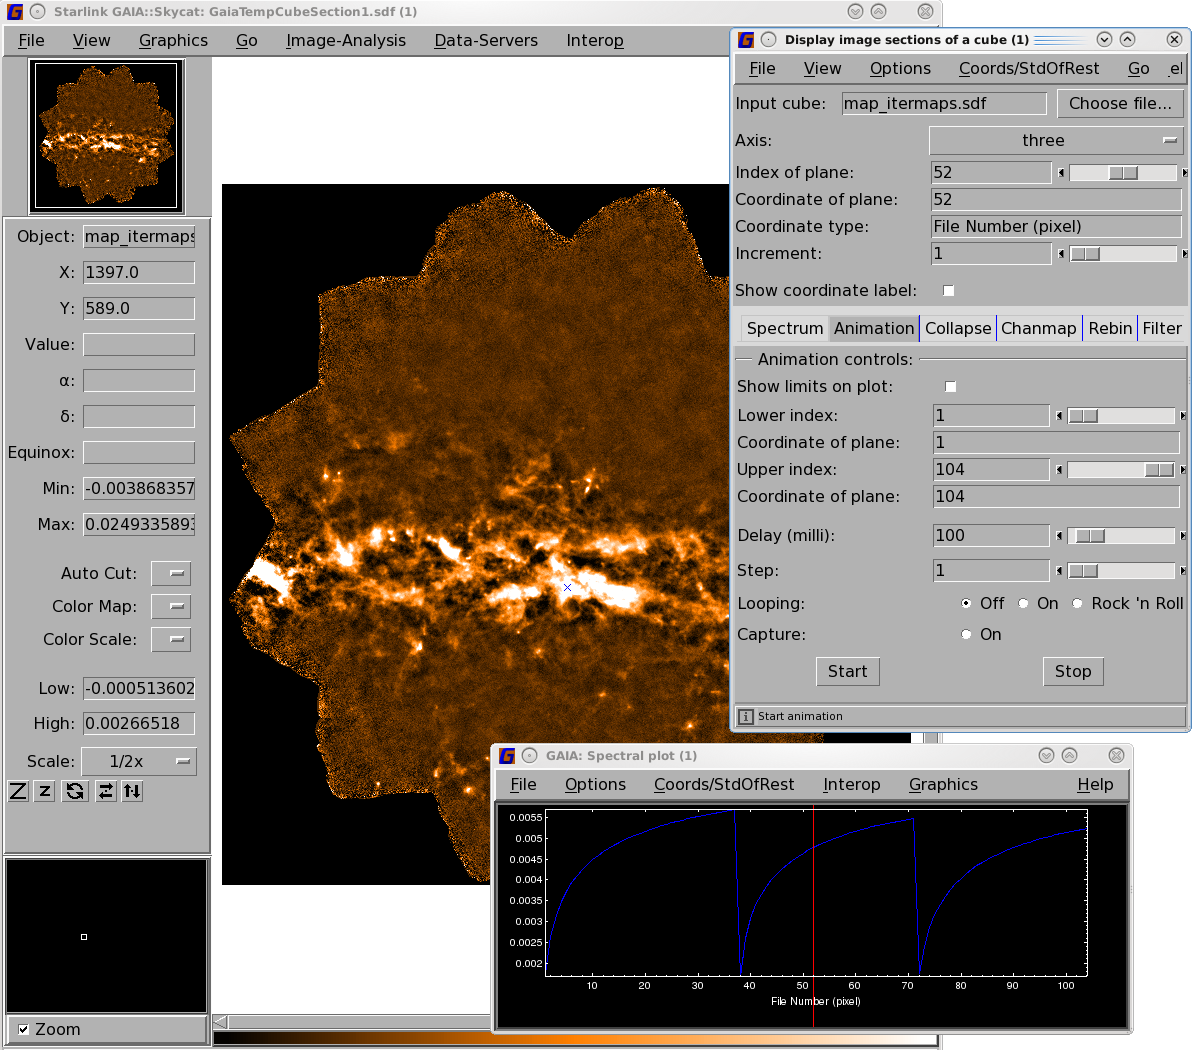
\includegraphics[width=0.95\textwidth]{sc21_itermaps_anim}

\end{minipage}
\hspace{0.3cm}
\begin{minipage}[c]{0.29\linewidth}
The output map map\_itermaps can be opened with \gaia. The data used
in this example is the Galactic map reduced in
\cref{Section}{sec:bright_ex}{dimmconfig\_bright\_extended.lis}. The
Spectral plot window shows the value for a single pixel and the 3
chunks are easily identified. You can select the `Animation' tab in
the `Display image sections' window and click `Start' to loop through
the itermaps for each iteration. the `movie' will appear in the main
\gaia\ window.
\end{minipage}

\vspace{0.7cm}

\begin{minipage}[c]{0.65\linewidth}
\centering
\hspace{0.5mm}
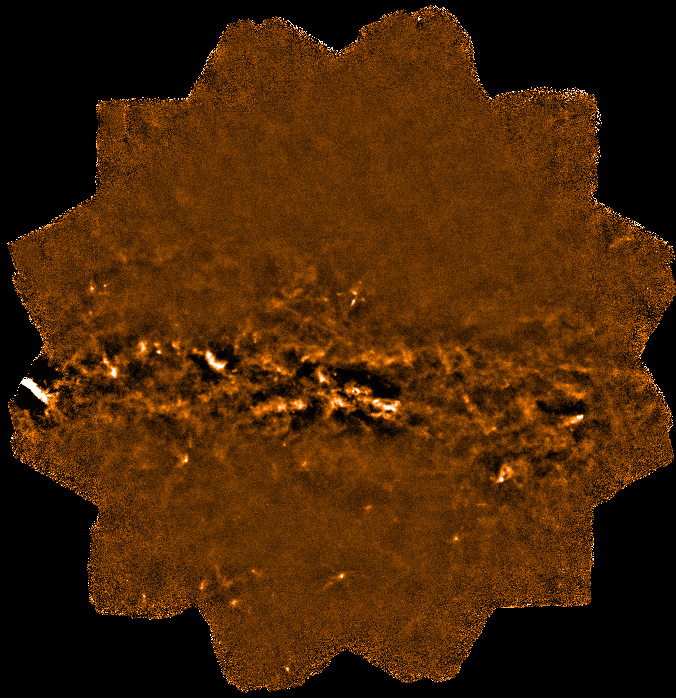
\includegraphics[width=3cm, height=3cm]{sc21_iter1}
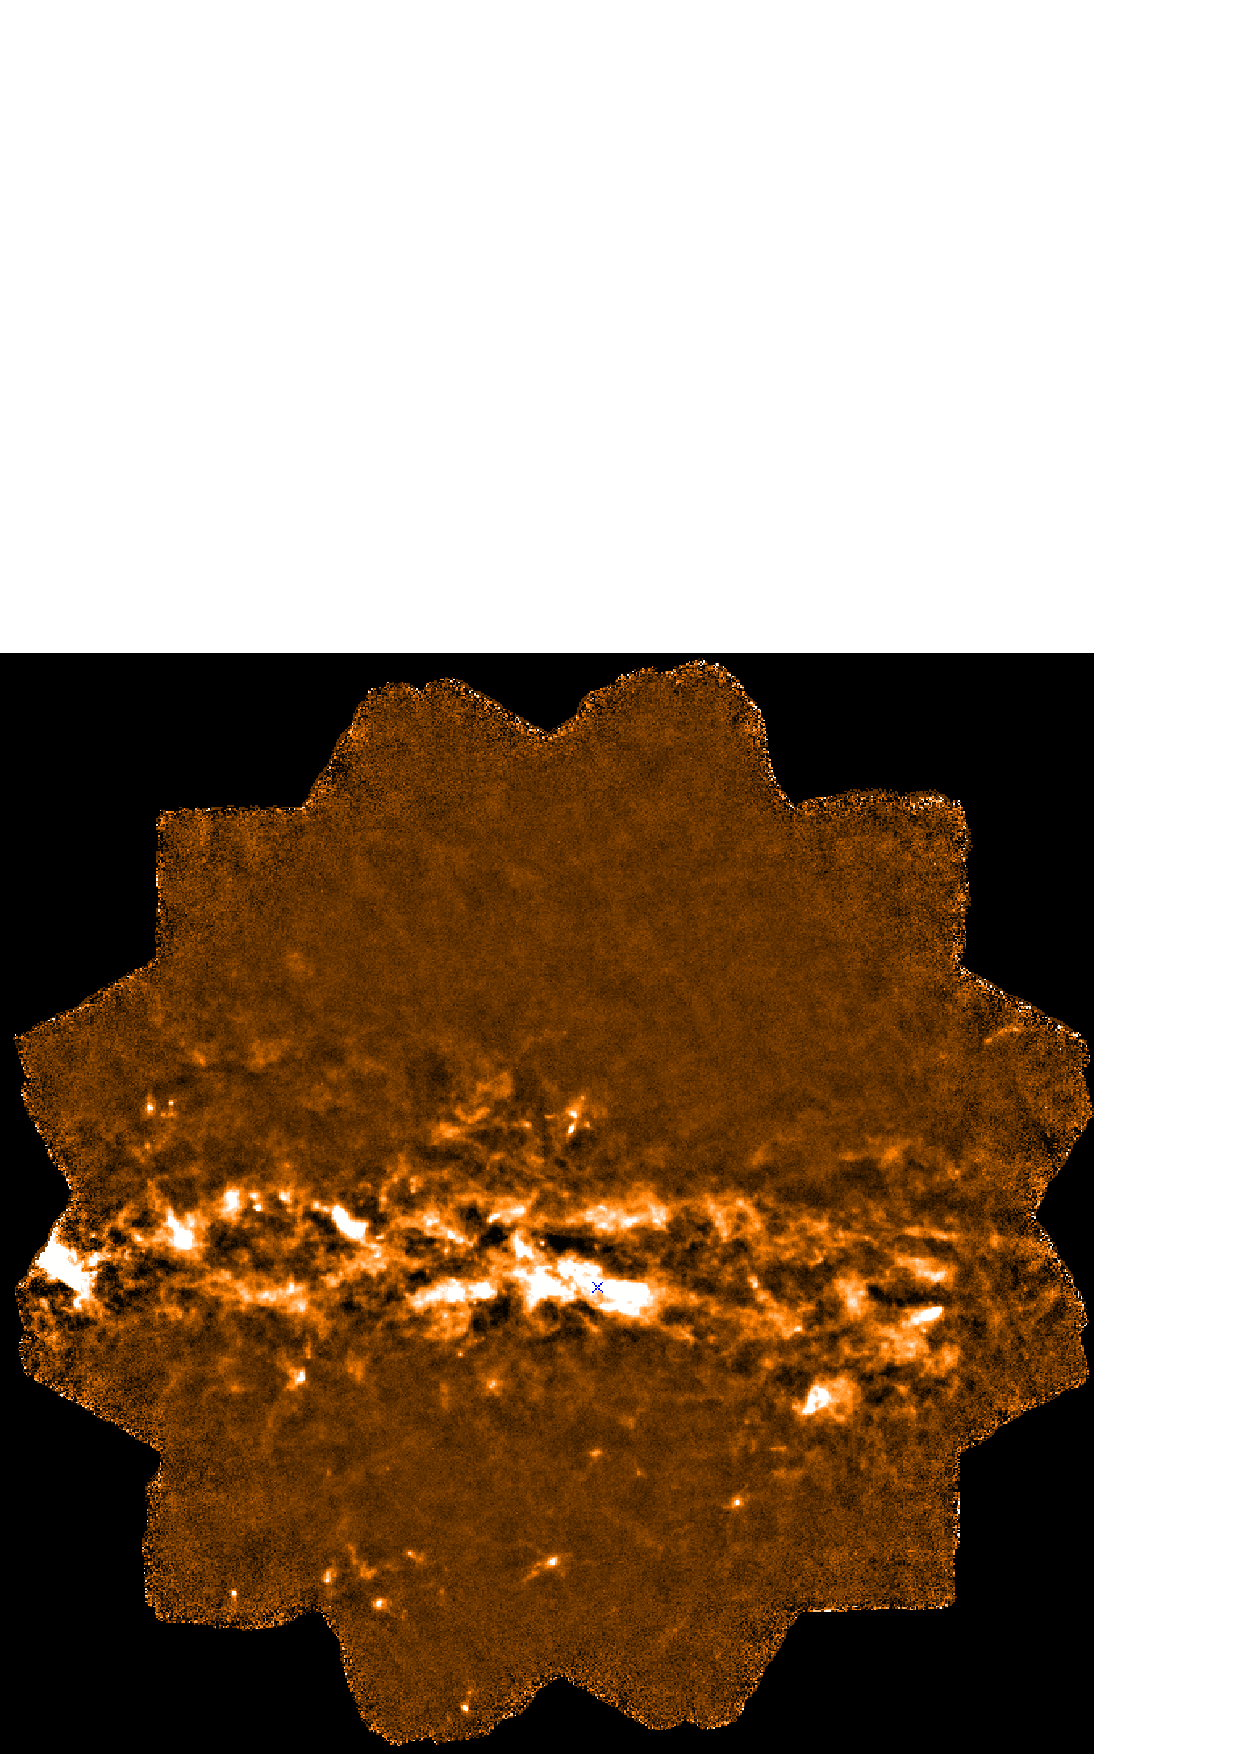
\includegraphics[width=3cm, height=3cm]{sc21_iter2}
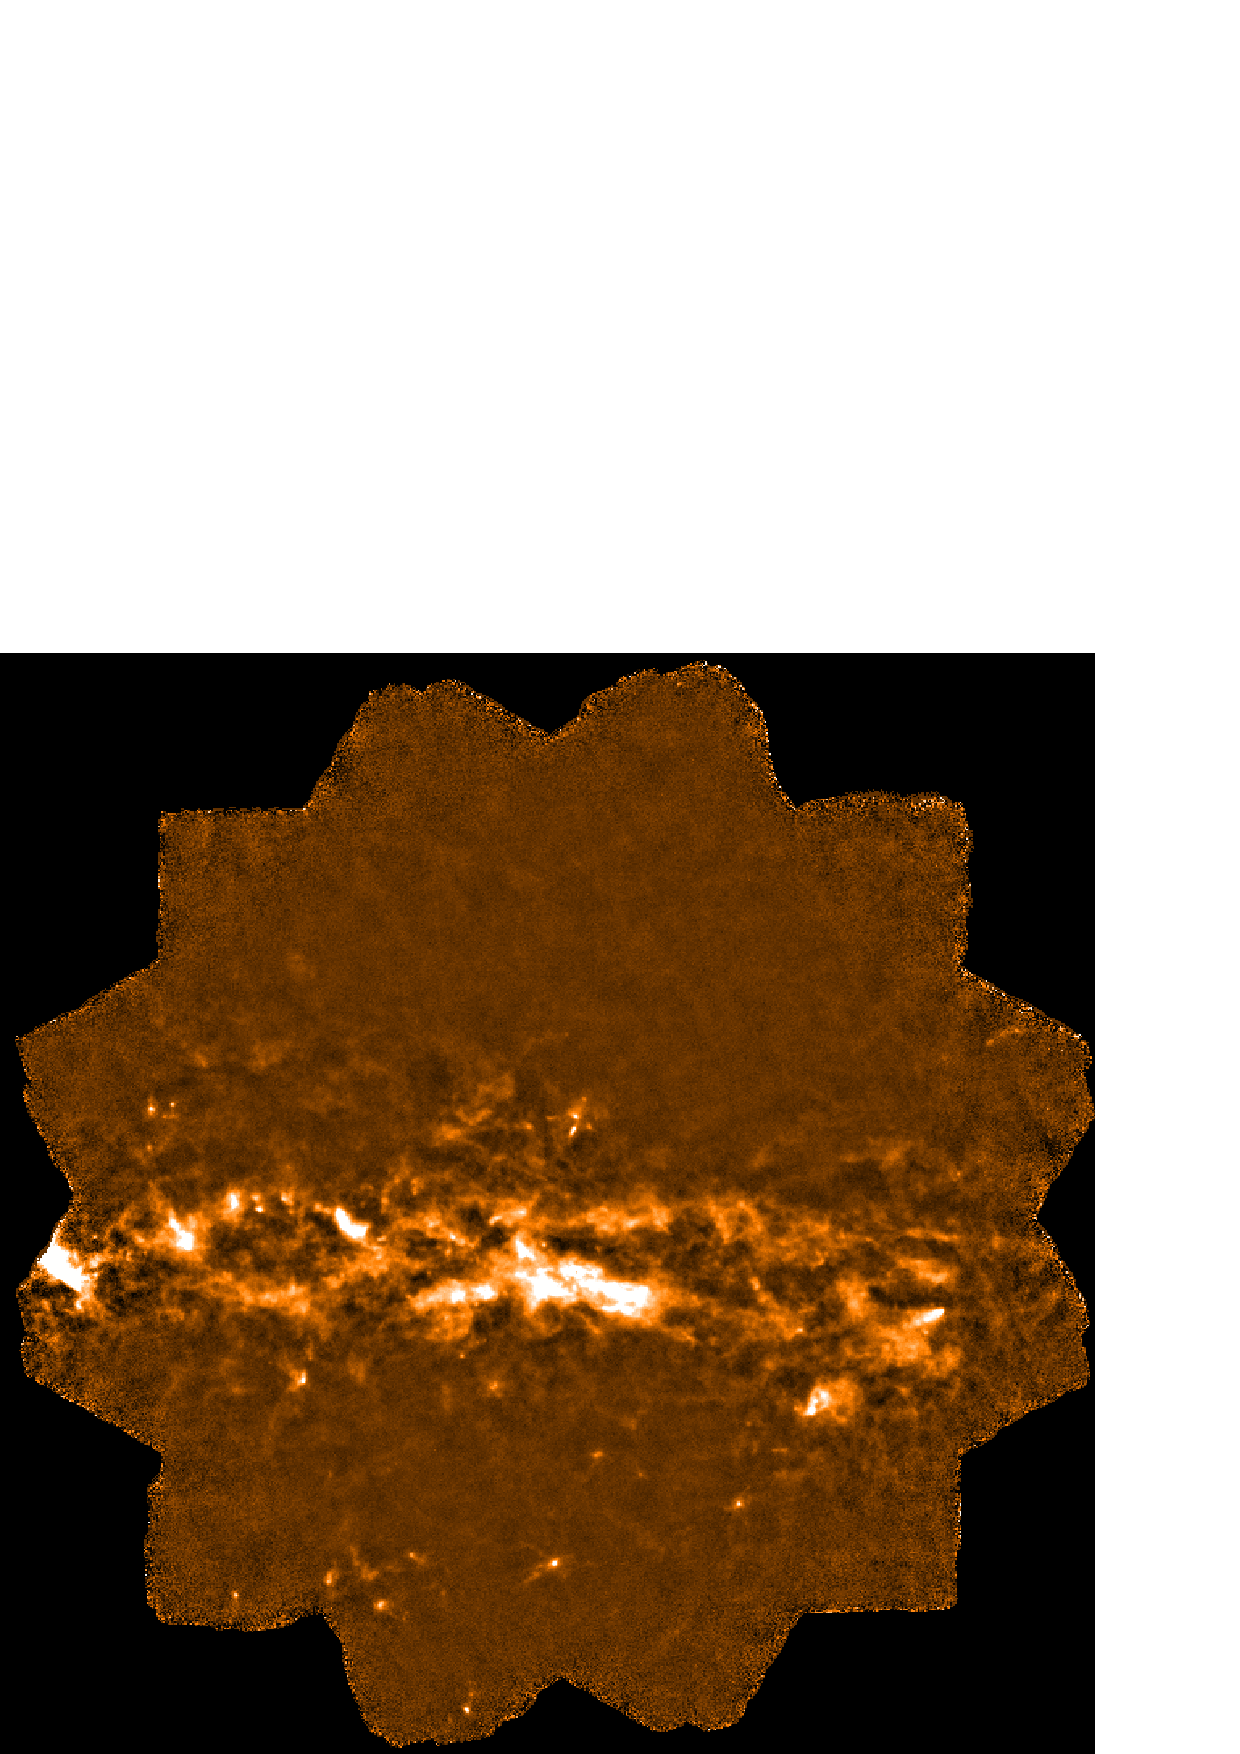
\includegraphics[width=3cm, height=3cm]{sc21_iter31}
\vspace{0.2cm}
\end{minipage}
\hspace{0.3cm}
\begin{minipage}[c]{0.29\linewidth}
These windows show the itermaps map at 1, 10, and 30 iterations. A
specific iteration can be selected using the `Index of plane' slider
on the `Display image sections' window.
\vspace{0.2cm}
\end{minipage}
\end{fmpage}
\end{center}
\caption{\small Example using the \smurf\ command \stackframes\ and
\gaia\ to view the `itermaps' map for each iteration.}
\label{fig:stack}
\end{figure}
\end{latexonly}

% The minipages used for the dvi version give latex2html problems.
\begin{htmlonly}
\label{fig:stack} \htmladdimg{sc21_view_itermaps.png}
Figure: Example using the \textsc{Smurf} command \task{stackframes} and
\gaia\ to view the `itermaps' map for each iteration.
\end{htmlonly}

\begin{myquote}
\begin{verbatim}
% gaia 850map.more.smurf.shortmaps
\end{verbatim}
\end{myquote}

\textbf{Note:} You can view the shortmaps and itermaps more
conveniently by stacking them into a single cube using the \smurf\
command \stackframes. This cube can then be viewed as a
`movie' with \gaia, using the animation option to loop through the
itermaps. See \cref{Figure}{fig:stack}{the box above} for instructions.

\subsection{\xlabel{filt}Adjusting the filtering}
\label{sec:filt}

Some of the most important parameters to experiment with are the
filtering options. By default the low-pass filter is applied once
during the pre-processing stage and is turned off for the iterative
steps. The high-pass filter is only specified during the iterative
steps and its selected value is crucial for maps containing extended
emission.  All the parameters dealing with the \texttt{FLT} model can
be found in \cref{Appendix}{app:par_full}{Configuration Parameters: dimmconfig.lis}.

The maximum spatial scale of structure that can be recovered by the
map-maker is determined by the scanning speed and frequency cut
applied to the data:

\begin{equation}
\frac{\mbox{speed}\;(''/\mbox{s)}}{\mbox{frequency cut}\;(\mbox{Hz)}}=\mbox{scale size}\;('')
\end{equation}

The filtering options set in \texttt{dimmconfig.lis} are:

\texttt{450.flt.filt\_edge\_largescale = 600} \\
\texttt{850.flt.filt\_edge\_largescale = 300}.

To make your life easier, these parameters allow you to specify the
filter limits in terms of spatial scale in arcsecs---in this case
300\,arcsec at 850\,$\mu$m and 600\,arcsec at 450\,$\mu$m. For example
at 850\,$\mu$m, recovering scales of 300\,arcsec at a scan speed of
600\,arcsec/sec (default for a 1 degree \textsc{pong}) corresponds to
a frequency 2\,Hz.

Choosing a high-pass filter is especially important for the recovery
of extended emission where you will likely wish to specify larger
spatial scales for \texttt{flt.filt\_edge\_largescale} than specified
by the default file. Indeed the
\texttt{dimmconfig\_bright\_extended.lis} recipe changes the
850\,$\mu$m value to \texttt{850.flt.filt\_edge\_largescale = 600}. Be
aware that increasing these scales simultaneously decreases the
flatness of your background. A compromise must be made between
extended structure and the flatness of your map. See
\cref{Figure}{fig:fltcompare}{the figure below} for an illustration of
the effect of \texttt{flt.filt\_edge\_largescale} on your map.

The scanning speeds are fixed for a given observing mode; you can find
out the speed at which your data were taken from the
\texttt{SCAN\_VEL} parameter in the FITS header (see
\cref{Section}{sec:fitsheader}{Headers and file structure}).


\myfigduo{sc21_brex_19}{sc21_brex_18}{}{width=0.46\linewidth}{fig:fltcompare}{7mm}{
Highlighting the effects of high-pass filtering on your map.
\textbf{(Left)} Map made with \texttt{850.flt.filt\_edge\_largescale =
300}. \textbf{(Right)} Map made with
\texttt{850.flt.filt\_edge\_largescale = 1000}. All other
configuration parameters remain the same.}

\subsection{\xlabel{fitcom}Fitting COM for each sub-array}
\label{sec:fitcom}

A useful option to improve the flatness of your maps is to fit the
\texttt{COM} model independently for each sub-array. This is
particularly effective if you find you have one sub-array noisier than
the others.

This comes with the warning however that you will lose information on
any scales larger than the area covered by a single sub-array. It is
therefore not recommended if you have very large-scale extended
structure.

To initialise this option set \texttt{com.perarray = 1}.


\subsection{\xlabel{noibox}Flagging bad data}
\label{sec:noibox}

It is possible to down-weight data that have higher noise by setting
the parameter \texttt{noi.box\_size}. If this is set (i.e. non-zero)
then the length of time over which the noise is determined can be
specified in time samples (positive values) or seconds (negative
values). By default this is set to zero and the whole time stream is
used giving a single variance for each bolometer. This variance is
used to weight the data for subsequent iterations, hence more finely
estimated noise levels are preferable.

Setting \texttt{noi.box\_size} helps remove `scuffs' or other noise
artifacts you might see in your error map due to a sub-array (or
arrays) temporarily jumping to a higher noise state. We recommend a
value of \texttt{noi.box\_size = -15} (i.e. half a sub-scan). As the
value tends to -1 (one second) we find some of the source signal being
down-weighted. Higher than this -15 value and the map-maker becomes
less sensitive to the higher noise states.

Other parameters you may want to utilise include \texttt{flagfast} and
\texttt{flagslow}. You may find that setting \texttt{flagfast} to less
than the default of 1000''/sec will help reduce the effect of any
`smearing' of sources (and of noise) in maps, while setting \texttt{flagslow} greater
than the default of 300''/sec helps to flatten the edges of maps. To
determine reasonable values for your dataset you should do \jcmtstate\
and view the scan speed using \topcat---see
\cref{Section}{sec:scan}{Displaying scan patterns} for details.

\subsection{\xlabel{mask}Masking options}
\label{sec:mask}

The \texttt{AST}, \texttt{FLT} and \texttt{COM} models each have a
number of common masking options. The main ones are
\texttt{xxx.zero\_circle}, \texttt{xxx.zero\_lowhits},
\texttt{xxx.zero\_snr} and \texttt{xxx.zero\_snrlo}. Masking comes
with different restrictions and sensitivities depending on the model
in question.

\texttt{AST} masking is the option we recommend. On each iteration the
map is constrained to zero at all points outside the masked region and
the \texttt{AST} model is estimated based only on data inside the
mask.

\texttt{FLT} masking is used to omit bright sources from the estimate
of the low frequency background subtracted from the residuals on each
iteration. This can help prevent ringing in the final map. SNR based
\texttt{FLT} masking cannot be used on the first iteration and
\texttt{FLT} masking should be used sparingly to aid convergence (it
is limited to the first 2 iterations by default by
\texttt{flt.zero\_niter = 2}).

\texttt{COM} masking is used to omit very bright sources from the
estimate of the common-mode signal, this can prevent sources being
rejected due to their dissimilarity to the common-mode. SNR based
\texttt{COM} masking cannot be used on the first iteration and the
mask should always be small.

For the rest of this section we will concentrate on \texttt{AST}
masking only. \texttt{ast.zero\_circle} defines a circle is defined to
mask out the source, with everything outside this circle being
constrained to zero. This is utilised in
\texttt{dimmconfig\_bright\_compact.lis} by the \texttt{AST} model as
the source is expected to be very compact with a flat background. The
default size of this circle is 60\,arcsec, but this can adjusted by
altering \texttt{ast.zero\_circle}. The position of this circle
defaults to the centre of the map. You can specify alternative
coordinates if this is not appropriate.

\texttt{ast.zero\_lowhits} allows masking based on the number of data
samples in a pixel. For the \texttt{AST} model this means that
spurious regions of emission at the edges of the map where exposure
time is low are not included in the source mask. See the documentation
in \cref{Appendix}{app:par_full}{Configuration Parameters:
dimmconfig.lis} for more information on each.

Finally there is signal-to-noise based masking as utilised by
\texttt{dimmconfig\_bright\_extended.lis}. It uses the parameter
\texttt{ast.zero\_snr} to define a mask based on the SNR. The default
is 5, meaning that pixels below an SNR of 5\,$\sigma$ will be set to
zero. This is dynamic with the SNR mask being re-determined after each
iteration. Setting \texttt{ast.zero\_snr} too low can cause noise
spikes to be interpreted as signal. Instead, \texttt{ast.zero\_snrlo}
can be set which allows the mask to grow to include pixels with an SNR
down to \texttt{ast.zero\_snrlo}. This typically improves the
resulting map so is well worth experimenting with.

An alternative to setting \texttt{ast.zero\_snrlo} is to smooth the
SNR mask by setting the parameter \texttt{ast.zero\_snr\_fwhm}.

Remember for all \texttt{AST} masking to include
\texttt{ast.zero\_notlast = 1} so that mask is not applied on the
final iteration. This means that the background regions in the map are
only generated by this single, final iteration.

An alternative to SNR masking is to supply an external mask using the
\texttt{REF} parameter.  Setting the parameter
\texttt{ast.zero\_snr\_fwhm} allows you to automate this step for a
specific case. Here, the map-maker is run once, then the mask
generated by \texttt{ast.zero\_snr} is smoothed by a Gaussian (of
`FWHM' arcsecs) and the map-maker is re-run with this smoothed mask
supplied as an external mask. You can supply your own external mask
however by following the instructions in the next section.

Multiple masks are combined according to the \texttt{ast.zero\_union}
parameter (there are also corresponding \texttt{FLT} and \texttt{COM}
ones). If this parameter is true (i.e. non-zero) then the two masks
will be combined to act as one large mask (the union of the individual
masks). Hence a pixel will be flagged/masked if it falls within either
mask (rather than being required to fall in both). The alternative is
a false (i.e. zero) value; this means that only pixels that fall into
both masks independently will be flagged/masked. Here, only the
intersection of the masks is considered the final masked area.

For example, if you find an SNR mask allow bright regions to develop
towards the edges of your map, you can force these to zero by using
the intersection of the SNR mask with a `low-hits' mask.

\subsection{\xlabel{maskbe}Supplying an external mask}
\label{sec:maskbe}

As an SNR mask is redetermined after each iteration it varies as the
map varies which can sometimes cause convergence problems. The mask
will also depend on the amount of data going into the map and the
pixel size. An externally supplied mask is fixed and tells the
map-maker where you expect the emission to be.

The sequence below is a summary of the procedure for generating and
supplying an external mask. In this example the mask is generated from
the map produced by an initial run through the map-maker.
Alternatively maps from other telescopes can be used.

These steps are followed in the example in \cref{Section}{sec:bright_ex}{Extended galactic sources}.

\textbf{(a)} Generate a map covering your region. This may be by simply
running the map-maker on your data as shown below.
\begin{myquote}
\begin{verbatim}
% makemap in='s8*.sdf' out=850map method=iterate \
config='"^dimmconfig_bright_extended.lis"'
\end{verbatim}
\end{myquote}
The alternative is to access a map from a different dataset or even a
different telescope, e.g. a map downloaded from the Herschel Science
Archive. For instructions on converting from fits format to NDF see
\cref{Appendix}{app:convert}{Converting a Herschel map to NDF}.
\\*\\*
\textbf{(b)} Make a signal-to-noise map using the \Kappa\ command \makesnr.
\begin{myquote}
\begin{verbatim}
% makesnr 850map 850map_snr
\end{verbatim}
\end{myquote}
\textbf{(c)} This SNR map is thresholded to set everything below 3$\sigma$ to 0 and
everything above to 1.
\begin{myquote}
\begin{verbatim}
% thresh 850map_snr 850map_mask thrlo=3 newlo=0 thrhi=3 newhi=1
\end{verbatim}
\end{myquote}
In the step above you can set everything below 3$\sigma$ to
\texttt{bad} and use this as your mask. However this generates a hard
3$\sigma$ cut-off to your map which is unrealistic for the real data.
Instead the following 2 steps are performed to smooth the edges of the
mask.
\\*\\*
\textbf{(d)} The thresholded map is smoothed with a Gaussian filter
of FWHM of 5 pixels (=\,20\,arcsec). Then it is again thresholded, this time
keeping everything above 5\,\% of the 0 level as the mask and setting
the rest to \texttt{bad}.
\begin{myquote}
\begin{verbatim}
% gausmooth 850map_mask 850map_mask_sm fwhm=5
% thresh 850map_mask_sm 850map_mask_zm thrlo=0.05 newlo=bad thrhi=0.05 newhi=1
\end{verbatim}
\end{myquote}
Finally the map is re-made with this mask supplied as an external
file. Notice that the extra parameters required to pick up this external
mask are being appended to the configuration file on the command line
rather than editing the file itself.
\begin{myquote}
\begin{verbatim}
% makemap in='s8*.sdf' out=850map_zm method=iterate \
config='"^dimmconfig_bright_extended.lis,ast.zero_mask=1,ast.zero_snr=0"' \
ref=850map_mask_zm
\end{verbatim}
\end{myquote}

\subsection{\xlabel{skyloop}Skyloop}
\label{sec:skyloop}

Traditionally, the map-maker divides a non-contiguous sequence of time
series data into chunks. It processes each chuck independently
before coadding them as a final step in the the reduction.

This means for each chunk the map-maker has to start from scratch
determining the \texttt{AST} model and the benefit of long integration
times spent building up the signal is lost. Recipes which use
signal-to-noise masks especially suffer from this approach as the
signal-to-noise in each individual chunk can remain low and fainter
extended structure is not recovered.

This new \skyloop\ command runs \makemap\ multiple times
performing just a single iteration on each occasion. It starts by
performing a single iteration of \texttt{makemap} from which a final
coadded map is generated. This map is then supplied as an initial
estimate of the sky for the next loop through \texttt{makemap}. On
this next iteration, the initial sky estimate is subtracted from the
cleaned time-series data and the \texttt{COM}, \texttt{GAI},
\texttt{FLT}, \texttt{EXT} models are subtracted. This produces a new
model of the sky (from the current iteration) to which the sky
estimate (from the previous iteration) is then added. In this way the
signal from all of the chunks is built up over the iterations and is
all included in the final map estimate when convergence is reached.

Be aware that \texttt{skyloop} uses a lot of disk space. Setting
environment variable \texttt{STAR\_TEMP} to a suitable location
before you start will prevent \texttt{skyloop} from crashing
if you run out of temporary storage space.
\begin{myquote}
\begin{verbatim}
% setenv STAR_TEMP .
\end{verbatim}
\end{myquote}
 \texttt{skyloop} is then called in the same way as \texttt{makemap}, with
 a configuration file specified on the command line.
\begin{myquote}
\begin{verbatim}
% skyloop in=^myfiles.lis out=map_skyloop config=^dimmconfig_bright_extended.lis \
LOGFILE=skyloop.log ILEVEL=ATASK GLEVEL=debug
\end{verbatim}
\end{myquote}

\clearpage
\section{\xlabel{Examples}Examples of Different Reductions}
\label{sec:eg}

\subsection{\xlabel{Cosmology}Deep point-source maps}
\label{sec:cosmology}

The science goal of many extra-galactic SCUBA-2 observations is to
detect unresolved point sources. In the examples below we work through the
reduction of just such an extra-galactic field, A1835.

Most extra-galactic objects are on average only slightly brighter than
the confusion limit---the fluctuations of the background sky
brightness due to multiple super-imposed, unresolved sources within
the telescope beam, below which individual sources cannot be detected.
It is likely that any sources in the map will be at best, only a few
standard deviations brighter than the noise in the map (caused by a
combination of instrumental noise and source confusion).

\subsubsection{Example 1 - The simple reduction}
The basic reduction method for maps like these follow two main
steps---running the data through the map-maker using the
\texttt{dimmconfig\_blank\_field.lis} recipe (see
\cref{Section}{sec:config}{Specialised configuration files}). Then
applying the \picard\ \drrecipe{SCUBA2\_MATCHED\_FILTER} recipe (see
\cref{Section}{sec:mf}{Point-source extraction}).
\\ \\
\textbf{(a) Run the map-maker}\\
In this example the raw data is stored locally in a directory called
\texttt{data}. We have three observations (\#13, \#18, \#21) of the field
which we will reduced independently.

\begin{myquote}
\begin{verbatim}
% makemap data/s8*00013_00\*.sdf cosmo1 method=iterate \
config=^$STARLINK_DIR/share/smurf/dimmconfig_blank_field.lis

% makemap data/s8*00018_00\*.sdf cosmo2 method=iterate \
config=^$STARLINK_DIR/share/smurf/dimmconfig_blank_field.lis

% makemap data/s8*00021_00\*.sdf cosmo3 method=iterate \
config=^$STARLINK_DIR/share/smurf/dimmconfig_blank_field.lis

\end{verbatim}
\end{myquote}

\textbf{(b) Combine the maps}\\
These three maps are then combined using the \textsc{Picard} recipe
\xref{\drrecipe{MOSAIC\_JCMT\_IMAGES}}{sun265}{MOSAIC_JCMT_IMAGES}. In
this case we accept the default of \wcsmosaic\ mosaicking and
nearest-neighbour pixel spreading and so do not supply a parameter
file.
\begin{myquote}
\begin{verbatim}
% picard MOSAIC_JCMT_IMAGES cosmo*.sdf
\end{verbatim}
\end{myquote}
The output map, \texttt{cosmo2\_mos.sdf}, is shown in the left-hand
panel of \cref{Figure}{fig:cosmomap}{the figure below}. The advantage of using the
\textsc{Picard} recipe over standalone \Kappa\ commands is that the exposure
time is also propagated correctly to the output mosaic (it is stored
in the \texttt{MORE.SMURF.EXP\_TIME} extension).
\\

\myfigduo{sc21_850cosmo_bf}{sc21_850cosmo_mf_crop}{}{width=0.48\linewidth}{fig:cosmomap}{2mm}{
  Reduced \textsc{pong} maps of cosmology field A1835. \textbf{Left:}
  Map reduced with \texttt{dimmconfig\_blank\_field.lis}.
  \textbf{Right:} Map on the left after the matched filter has been
  applied and it has been cropped.}

\textbf{(c) Apply the matched filter}\\
In order to optimally find sources that are the size of the telescope
beam, we apply the matched filter recipe --
\xref{\drrecipe{SCUBA2\_MATCHED\_FILTER}}{sun265}{SCUBA2_MATCHED_FILTER}.
We create a simple parameter file called \texttt{smooth.ini}:
\begin{myquote}
\begin{verbatim}
[SCUBA2_MATCHED_FILTER]
SMOOTH_FWHM = 15
\end{verbatim}
\end{myquote}
where \texttt{SMOOTH\_FWHM = 15} indicates that the background should be
estimated by first smoothing the map and PSF with a 15-arcsec FWHM
Gaussian. Next, the recipe is executed as follows:
%
\begin{myquote}
\begin{verbatim}
% picard -recpars smooth.ini SCUBA2_MATCHED_FILTER cosmo2_mos.sdf
\end{verbatim}
\end{myquote}
%
The output of this operation is a smoothed image called
\texttt{cosmo2\_mos\_mf.sdf} and a cropped version is shown in the
right-hand panel of \cref{Figure}{fig:cosmomap}{figure above}. You can immediately
see the contrast to the left-hand panel which is the output from the
map-maker. A number of signal peaks now emerge as possible sources.
\\ \\
\textbf{(d) Crop the map}\\
Next we shall crop the map to remove the noisy edges,
in this case to a 900-arcsec radius circle. The output file will be named
\texttt{cosmo2\_mos\_mf\_crop.sdf}.
\begin{myquote}
\begin{verbatim}
% picard CROP_JCMT_IMAGES cosmo2_mos_mf.sdf

\end{verbatim}
\end{myquote}

\myfig{sc21_850cosmo_mf_crop_snr}{}{width=0.6\linewidth}{fig:snrmask}{
  Signal-to-noise map made the \Kappa\ command \makesnr.
  The map has been scaled from 0 to +3.}

\textbf{(e) Make an SNR map}\\
Finally, we need to find sources. The filtered map contains a
VARIANCE component, so it is easy to produce an SNR map using the
\textsc{Kappa} task \task{makesnr}:
\begin{myquote}
\begin{verbatim}
% makesnr cosmo2_mos_mf_crop cosmo2_mos_mf_crop_snr
\end{verbatim}
\end{myquote}

The resulting map, \texttt{cosmo2\_mos\_mf\_snr}, is shown in
\cref{Figure}{fig:snrmask}{signal-to-noise image}. Compared with the
matched filter map the
edges no longer appear as noisy because they have been down-weighted
by the larger noise values where there were less data.
\\ \\
\textbf{(f) Identify sources}\\
The basic procedure for identifying sources would be to locate peaks
above some threshold SNR. The SNR image above shows peaks that are
likely to be real sources. For a start, a source appears where
expected at the 0,0 position.

But how can we check if these sources are real?
\begin{itemize}

\item One option is to split your data into mutually exclusive subsets
  and produce independent maps. Are the highest SNR peaks detected in each of
  them?
\item A second test is to compare the number of {\em negative} peaks above
  a given SNR with the number of {\em positive} peaks.
\end{itemize}

\subsubsection{Example 2 - Advanced pipeline method}
\label{sec:jk}

Although this method is considerably simpler to execute, the products
have undergone more advanced processing than the manual method just
given. The pipeline is particularly recommended for this recipe due to
its extra analysis steps.

\textbf{(a) Create input file}\\
Create an file with the names of all the files you wish to process (e.g. myfiles.lis)
\\ \\
\textbf{(b) Run the pipeline}\\
The pipeline must first be initiated for the wavelength you are
working on. In the case below this is 850\,$\mu$m. Note that the date
does not \emph{have} to be specified when initialising the pipeline.
The pipeline is run using the
\xref{\drrecipe{FAINT\_POINT\_SOURCES\_JACKKNIFE}}{sun265}{FAINT_POINT_SOURCES_JACKKNIFE}
recipe; this uses \texttt{dimmconfig\_blank\_field.lis} as the
configuration file. If you wish to provide an alternative file you
will need to put the name of the new configuration file in a recipe
parameter file---see \cref{Section}{sec:runpl}{The SCUBA-2 Pipeline}
for details.
\begin{myquote}
\begin{verbatim}
% oracdr_scuba2_850 -cwd YYYYMMDD
% oracdr -loop file -files myfiles.lis -nodisplay \
-log sf FAINT_POINT_SOURCES_JACKKNIFE
\end{verbatim}
\end{myquote}


The pipeline will write out a large number of files with the following suffices:

\begin{minipage}[t]{0.3\linewidth}
sYYYYMMDD*\_fmos
sYYYYMMDD*\_mappsf\\\\
gsYYYYMMD*\_wmos
gsYYYYMMD*\_whiten
gsYYYYMMD*\_cal
gsYYYYMMD*\_mf
\end{minipage}
\begin{minipage}[t]{0.7\linewidth}
The map for each observation\\
The map for each observation with an artificial\\point source added at the map centre\\
The coadd of all the \_fmos files\\
The whitened version of \_wmos\\
The calibrated version of \_whiten\\
The matched-filtered version of \_cal\\
\end{minipage}

\drrecipe{FAINT\_POINT\_SOURCES\_JACKKNIFE} is a recipe designed to
process blank field/extra-galactic data. The recipe uses a jack-knife
method to remove low-spatial frequency noise and generate a matched
filter output map.

The recipe processes each observation twice, a standard reduction
first, then a re-run with a fake point source added to the time
series. This produces a coadded signal map (\_wmos) and a
coadded PSF map (\_mappsf).

After the map-maker has completed, the recipe will call
\xref{\drrecipe{SCUBA2\_JACKKNIFE}}{sun265}{SCUBA2_JACKKNIFE}. This
routine divides the observations into two groups (odd and even) which
are coadded and then subtracted to create a jack-knife map. This map
contains only noise with no contribution from astronomical signal. The
angular power spectrum of this map is then used to estimate and remove
the residual 1/\emph{f} noise from the signal map and the PSF map;
this is the whitening step. The whitened jack-knife map is run through
\xref{\drrecipe{SCUBA2\_MATCHED\_FILTER}}{sun265}{SCUBA2_MATCHED_FILTER}
using the whitened PSF map as the PSF input. It is this matched filter
map which will be of most interest to users.

See \pipelinesun\ for more information on
\drrecipe{FAINT\_POINT\_SOURCES\_JACKKNIFE} and all other pipeline
recipes \\ \\ \textbf{(c) Optional: Re-run
\drrecipe{SCUBA2\_JACKKNIFE}}\\

You may wish to run the \drrecipe{SCUBA2\_JACKKNIFE} step again
independently from the pipeline. If your final map does not look as
expected you might first examine the individual mosaics from the
pipeline (\_fmos), one of these observations might show visible
artifacts that you wish to exclude from the coadd. The size of the
region in the jackknife image which is used to do the whitening step
is determined automatically, but the method may fail if the box is too
small.

If you decide to re-run this step you first coadd all the `\_mappsf'
files to create a coadded PSF using the \picard\ recipe
\xref{\drrecipe{MOSAIC\_JCMT\_IMAGES}}{sun265}{MOSAIC_JCMT_IMAGES}.
\begin{myquote}
\begin{verbatim}
% picard MOSAIC\_JCMT\_IMAGES *_mappsf
\end{verbatim}
\end{myquote}
Next create a parameter file (\texttt{recpars.lis}) for the jack-knife
recipe (\drrecipe{SCUBA2\_JACKKNIFE}) with the following:
\begin{myquote}
\begin{verbatim}
[SCUBA2_JACKKNIFE]
PSF_MATCHFILTER = <name_of_above_coadded_PSF>.sdf
\end{verbatim}
\end{myquote}
Another option for this parameter file is `WHITEN\_BOX' to set the
size of the region used to calculate the angular power spectrum.
Finally run \drrecipe{SCUBA2\_JACKKNIFE}:
\begin{myquote}
\begin{verbatim}
% picard -log sf -nodisplay -recpars recpars.lis SCUBA2_JACKKNIFE *fmos.sdf
\end{verbatim}
\end{myquote}
This will create files beginning with pgYYYMMDD$\ldots$ that should have
the same suffices as above: \_wmos, \_whiten, \_cal and \_mf.


\subsection{\xlabel{Galactic}Extended Galactic sources}
\label{sec:bright_ex}

This example is concerned with recovering bright extended emission.
The signal from extended emission varies slowly as seen by the array
passing over it. It thus appears at lower frequencies in the power
spectrum and complicates the high pass filter selection. Too harsh a
filter will make flat maps but any extended emission will have been
removed in doing so.
\\ \\
\textbf{(a) Running the map-maker}\\
We run the map-maker using \texttt{dimmconfig\_bright\_extended.lis};
we have also specified a couple of overrides on the command line --
\texttt{maptol}=0.04 is slightly more stringent than default and
\texttt{ast.zero\_snrlo = 3} allows the 5\,$\sigma$ mask set by the
configuration file to grow out to an SNR of 3\,$\sigma$; however, it
will only expand to include adjacent pixels.

In this example we give the map-maker a file containing a list of the
input files (filelist.txt) and
\texttt{dimmconfig\_bright\_extended.lis} is in the local directory.

\begin{myquote}
\begin{verbatim}
% makemap in=^filelist.txt 850galactic method=iterate \
config='"^dimmconfig_bright_extended.lis,maptol=0.04,ast.zero_snrlo=3"'
\end{verbatim}
\end{myquote}

\myfig{sc21_gal_11}{[t!]}{width=0.6\linewidth}{fig:galmakemap}{
  The output from the map-maker using \texttt{dimmconfig\_bright\_extended.lis}.}

\textbf{(b) Generating an external mask}\\
It is likely the first step, with the inclusion of
\texttt{ast.zero\_snrlo}, will produce a perfectly good map and you
may decide subsequent steps may be unnecessary. Nevertheless this
example will cover the other main techniques if you wish to experiment
further with masking options.

Next we create an external mask from the output of \makemap. Here we
follow the steps outlined in \cref{Section}{sec:mask}{Masking options}.

\begin{myquote}
\begin{verbatim}
% makesnr 850map 850map_snr
\end{verbatim}
\end{myquote}

This SNR map is thresholded to set everything below 3\,$\sigma$ to 0 and
everything above to 1.

\begin{myquote}
\begin{verbatim}
% thresh 850map_snr 850map_mask thrlo=3 newlo=0 thrhi=3 newhi=1
\end{verbatim}
\end{myquote}
The thresholded map is shown in the left-hand panel of
\cref{Figure}{fig:mask}{this figure}. The next step is to smooth this
map by multiplying it with a Gaussian of 16\,arcsec. For this we use a
factor of 4 for the FWHM parameter.

\begin{myquote}
\begin{verbatim}
% gausmooth 850map_mask 850map_mask_sm fwhm=4
\end{verbatim}
\end{myquote}

We threshold the map again to produce our mask. In this case all
values below out threshold are set to `bad'. The the smoothed map now
has values scaled between 0 and 1, we set our threshold at 0.02 to
include more of the emission beyond the 3\,$\sigma$ edge.
\begin{myquote}
\begin{verbatim}
% thresh 850map_mask_sm 850map_mask_zm thrlo=0.02 newlo=bad thrhi=0.02 newhi=1
\end{verbatim}
\end{myquote}
The final mask is shown in the right-panel of \cref{Figure}{fig:mask}{this figure},
note how it encompasses more emission and has softer edges than the
first threshold map. \\

\myfigduo{sc21_gal_mask1}{sc21_gal_mask2}{}{width=0.475\linewidth}{fig:mask}{2mm}{
  \textbf{(left)} The initial mask created by thresholding 850map\_snr
  to 3\,$\sigma$. \textbf{(right)} Second mask made by thresholding the
  smoothed map to 0.02.}

\textbf{(c) Re-running the map-maker with an external mask supplied}\\
As a last step the map is re-made with this mask supplied as an external
file. For this run we apply the additional parameters in a
personalised configuration file, \texttt{mydimmconfig.lis}.
\begin{myquote}
\begin{verbatim}
% makemap in=^filelist.txt 850galactic method=iterate \
config=^mydimmconfig.lis ref=850map_mask_zm
\end{verbatim}
\end{myquote}

The configuration file, \texttt{mydimmconfig.lis}, has the following
format---note how it is based on
\texttt{dimmconfig\_bright\_extended.lis}. It has decreased the
convergence parameter to \texttt{MAPTOL}=0.03 but increased the number
of iterations to compensate as 40 is unlikely to be sufficient.
\begin{myquote}
\begin{verbatim}
^$STARLINK_DIR/share/smurf/dimmconfig_bright_extended.lis
numiter = -100
maptol = 0.03
ast.zero_mask=1
ast.zero_snr = 0
\end{verbatim}
\end{myquote}

\textbf{(d) Cropping the map}\\
We shall now crop the map to remove the noisy edges using the \picard\
recipe \xref{\drrecipe{CROP\_JCMT\_IMAGES}}{sun265}{CROP_JCMT_IMAGES}.
To determine what to trim we can look at the exposure-time image with
\gaia.

\cref{Figure}{fig:exptime}{The exposure-time image} shows a sharp drop
off at a radius of 30\,arcmin. We can thus specify a parameter file
(\texttt{recpars.ini}) and run \drrecipe{CROP\_JCMT\_IMAGES} like so:

\begin{myquote}
\begin{verbatim}
[CROP_JCMT_IMAGES]
MAP_RADIUS = 1800
\end{verbatim}
\end{myquote}

\begin{myquote}
\begin{verbatim}
% picard -recpars recpars.ini CROP_JCMT_IMAGES 850galactic.sdf
\end{verbatim}
\end{myquote}
The final cropped map is shown in \cref{Figure}{fig:crop_map}{this plot}. Compared
with the first map out of the map-maker
(\cref{Figure}{fig:galmakemap}{first map}),
slightly more of the faint extended emission is apparent.

One of the challenges facing this type of reduction is the need to
account for both faint extended structure and very bright sources in
the same map. You may find some degree of bowling remains around the
brightest sources.

\myfig{sc21_gal_exptime}{[t!]}{width=0.7\linewidth}{fig:exptime}{
The exposure-time image of the science map from
\cref{Figure}{fig:galmakemap}{this figure}. You can right-click and drag the mouse
between two points to measure the distance. Here we see the exposure
time dropping off sharply at a radius of 30\,arcmin. A non-default
colour scale has been chosen to illustrate the morphology.}

A patchy looking background is a result of the more relaxed high pass
filtering and is an inevitable consequence of recovering extended
emission. To remove that is to also remove extended emission as they
are essentially indistinguishable.

There are areas you may wish to experiment with:
\begin{itemize}
\item Adjust the filtering---see \cref{Section}{sec:filt}{Adjusting the filtering} for details.
\item Supply an external mask from a different dataset, e.g. a \htmladdnormallink{Herschel}{http://herschel.esac.esa.int/} map.
\item Run Skyloop---see \cref{Section}{sec:skyloop}{Skyloop} for details.
 \end{itemize}

\myfig{sc21_gal12_crop}{[t!]}{width=0.8\hsize}{fig:crop_map}{
The final cropped, reduced map from the map-maker run with
an external mask supplied.}


\clearpage
\section{\xlabel{pipeline}The SCUBA-2 Pipeline}
\label{sec:pipe}
\subsection{\xlabel{pl_overview}Pipeline overview}

SCUBA-2 data reduction pipelines have been developed based on the
existing \oracdr\ pipeline (Cavanagh et al., 2008\cite{oracdr}) used
for ACSIS. There are three distinct pipelines currently utilised by
SCUBA-2: two of these, the quick-look (QL) and summit pipelines, are
run in real time at the JCMT during data acquisition; the third, the science
pipeline, offers a comprehensive reduction which users will be
interested in running locally.

\begin{itemize}
\item The QL runs quality assurance checks on the data as it comes in.
For science data it calculates the noise between 2\,Hz and 10\,Hz,
along with the NEP and effective NEP, for each 30-second scan. These
values undergo quality assurance checks to ensure SCUBA-2 is within
an acceptable operating range.
\item The summit pipeline is designed to provide a quick map of the
data, it does this by running fewer iterations and chunking the data
more. This is a useful guide to observers who wish to check the
quality of their data.
\item The science pipeline is run the following day. Data from the
previous night is processed using an optimal reduction routine, that
includes the map-maker and a number of post-processing steps (outlined
below). These data are transferred to CADC and available for download
by project members the following day.
\end{itemize}

The manual for the SCUBA-2 pipeline can be found at \pipelinesun,
while the pipeline software comes as part of the \starlink\ suite.


\subsection{\xlabel{science_pl}The Science Pipeline}
The science pipeline will automate many of the steps discussed in
\cref{Section}{sec:maps}{Reducing your data}:
\vspace{-0.3cm}
\begin{itemize}\itemsep-0.3em
\item Run the iterative map-maker.
\item Apply the FCF to calibrate to mJy/beam.
\item Coadd multiple observations of the same object.
\item Apply the matched-filter if the blank-field configuration file
has been requested.
\end{itemize}

\subsection{\xlabel{running_pl}Running the Science Pipeline}
\label{sec:runpl}
\begin{minipage}[t]{0.05\linewidth}
\textbf{(1)}
\end{minipage}
\begin{minipage}[t]{0.95\linewidth}
The first step is to initialise the pipeline software. This is simply done by:
\begin{myquote}
\begin{verbatim}
% oracdr_scuba2_850 -cwd

\end{verbatim}
\end{myquote}
\end{minipage}

\begin{minipage}[t]{0.05\linewidth}
\textbf{(2)}
\end{minipage}
\begin{minipage}[t]{0.95\linewidth}
Next there are a few environment variables that must be defined to
ensure the data is read from and written to the right places. Many are
set automatically when the pipeline is initialised but others must be
set manually. Details of the optional variables are given in
\pipelinesun\ but the three mandatory ones are:
\begin{itemize}\itemsep-0.1em
\item \param{STARLINK\_DIR}: Location of your Starlink installation.
\item \param{ORAC\_DATA\_IN}: The location where the data should be read from.
If you are supplying a text file listing the raw data this should be the
location of that file.
\item \param{ORAC\_DATA\_OUT}: The location where the data products should be
written. Also used as the location for a user-specified configuration file.\\
\end{itemize}
\end{minipage}

\begin{minipage}[t]{0.05\linewidth}
\textbf{(3)}
\end{minipage}
\begin{minipage}[t]{0.95\linewidth}
You can find out which recipe has been assigned to your raw data via
the \texttt{RECIPE} parameter in the FITS header in any of your raw
files. This is the recipe which will selected automatically by the
pipeline for the reduction. For example:
\begin{myquote}
\begin{verbatim}
% fitsval s8a20120725_00045_0003.sdf RECIPE
\end{verbatim}
\end{myquote}

If you wish to supply a modified configuration file (in the examples
below called \texttt{myconfigfile.lis}) you should create a parameter
file (in the examples below called \texttt{mypars.ini}) which follows
the \picard\ format. However, instead of a \picard\ command name, you
insert the reduction recipe name assigned to your data and the new
configuration filename as the \texttt{MAKEMAP\_CONFIG} option. For
example, \texttt{mypars.ini} contains the following:

\begin{myquote}
\begin{verbatim}
[REDUCE_SCAN]
MAKEMAP_CONFIG = myconfigfile.lis

\end{verbatim}
\end{myquote}

\end{minipage}

\begin{minipage}[t]{0.05\linewidth}
\textbf{(4)}
\end{minipage}
\begin{minipage}[t]{0.95\linewidth}
Now you are ready to run the pipeline command, this example we use the
\texttt{-recpars} option to specify parameter file from which call an
external parameter file to call our modified configuration file:
\begin{myquote}
\begin{verbatim}
% oracdr -loop file -files inputlist.txt -log xf -recpars mypars.ini
\end{verbatim}
\end{myquote}
\end{minipage}

\subsection{\xlabel{pl_output}Pipeline recipes}
\label{sec:recipes}

Outlined below are the four primary \oracdr\ recipes observers are
likely to require.  The first three cover reducing science maps using
\texttt{makemap} and the specialised configuration files discussed in
\cref{Section}{sec:config}{Specialised configuration files}. The last
recipe, ASSESS\_DATA\_NOISE, is a diagnostic routine rather than a
reduction one. A complete description of all these recipes can be
found in \pipelinesun.


\subsubsection{\xlabel{extsources}REDUCE\_SCAN\_EXTENDED\_SOURCES}

This is the recipe for processing extended sources, with the
\texttt{dimmconfig\_bright\_extended.lis} configuration file called by
\makemap. Multiple observations are coadded and the output
map is calibrated in units of mJy/arcsec$^2$. This recipe also
performs a source finder routine; the results are written as a FITS
catalogue (with file extension \texttt{.FIT}) which can be read as a
local catalogue into \gaia.

\subsubsection{\xlabel{faint}REDUCE\_SCAN\_FAINT\_POINT\_SOURCES}

This is the recipe for processing maps containing faint compact
sources. This time the configuration file called by \texttt{makemap}
is \texttt{dimmconfig\_blank\_field.lis}. The resulting map is further
processed with a matched filter to give the first output map. Then the
signal-to-noise ratio is taken to enhance point sources, this
signal-to-noise map is written out as a second output file. This
recipe also performs a source finder routine; the results are written
as a FITS catalogue (with file extension \texttt{.FIT}) which can be
read as a local catalogue into \gaia.

\subsubsection{\xlabel{faintjk}FAINT\_POINT\_SOURCES\_JACKKNIFE}

This recipe uses a jack-knife method to remove residual low-spatial
frequency noise and create an optimal matched-filtered output map. The
map-maker is run twice, first as a standard reduction using
\texttt{dimmconfig\_blank\_field.lis}, and the second time with a fake
source added to the time series. This creates a signal map and an
effective PSF map. A jack-knife map is generated from two halves of
the dataset and the maps are `whitened' by the removal of the residual
1/\emph{f} noise. The whitened signal map is processed with the
matched filter using the whitened PSF map as the PSF input. The data
are calibrated in mJy/beam using a corrected FCF. See
\cref{Section}{sec:jk}{Example 2 - Advanced pipeline method} for a
more-detailed description of this recipe and the files produced.

\subsubsection{\xlabel{assessnoise}ASSESS\_DATA\_NOISE}

This recipe is designed to provide a simple assessment of the noise
properties of your data. It calculates the noise for either the first
on-sky data file (default) or for the entire time stream. The results
are passed through the same quality-assurance checks as performed by
the quick-look pipeline and a log files is written out (of the form
log.scinoise850). This log file reports the noise or weighted NEP and
number of bolometers. The formatting is designed to allow easy
plotting of any of these parameters vs time or sub-scan using \topcat\
for each subarray. The recipe also writes out other files ---
\texttt{log.bolonoise}, \texttt{index.noise} and \texttt{index.nep}.
From these files it will be possible to determine which files failed
the QA tests, and you may wish to exclude from the input list to the
map-maker.

\subsection{\xlabel{pl_output}Pipeline output}

The pipeline will produce a group file for each object being
processed. If the pipeline is given data from multiple nights, all
those data will be included in the group coadd using inverse variance
weighting.

The final maps in your output directory will have the suffix
\texttt{\_reduced}. Maps will be made for individual observations,
which will start with an \texttt{s} (e.g.
\texttt{s20120720\_00030\_850\_reduced.sdf}). Group maps, which may contain
coadded observations from a single night, are also produced which
have the prefix \texttt{gs} (e.g. \texttt{gs20120720\_30\_850\_reduced.sdf}).

\textbf{Note:} A group file is \emph{always} created, even if only a single
observation is being processed.

Additionally, PNG images are made of the reduced files at a variety of
resolutions.

\subsection{\xlabel{cadc}Getting your data from CADC}

The JCMT Science Archive is hosted by The Canadian Astronomy Data
Centre (CADC). Both raw data and data processed by the science pipeline
are made available to PIs and co-Is through the CADC interface
(\texttt{http://www3.cadc-ccda.hia-iha.nrc-cnrc.gc.ca/jcmt/}).

To access proprietary data you will need to have your CADC username
registered by the JAC and thereby associated with the project code.

When searching the JCMT Science Archive, be sure to select the correct
search option from the `JSA Queries' tab. Here you can select public
versus proprietary, raw versus reduced, and SCUBA-2 versus ACSIS data.

An important search option to be aware of is `Group Type', where your
options are Simple, Night, Project and Public. Simple (which becomes
`obs' on the result page) is an individual observation; night means
the group file from the pipeline (these may or may not include more
than one observation; the `Group Members' value will tell you), the
project option is generated if an entire project has been run through
the pipeline and identical sources across the project are coadded
into master group files.  However, project processing has yet to be
implemented.


\clearpage


\begin{thebibliography}{}
\addcontentsline{toc}{section}{References}

\bibitem{archibald}
Archibald,~E.~N., et~al, 2002, \htmladdnormallink{\textit{On the atmospheric limitations
of ground-based submillimetre astronomy using array receivers}}{
http://dx.doi.org/10.1046/j.1365-8711.2002.05582.x}, MNRAS, 336, 1-13
(DOI:10.1046/j.1365-8711.2002.05582.x)

\bibitem{oracdr}
Cavanagh~B., Jenness~T., Economou~F., Currie~M.~J., 2008,
\htmladdnormallink{\textit{The ORAC-DR data reduction
pipeline}}{http://dx.doi.org/10.1002/asna.200710944}, Astron. Nactr., 329, 295
(DOI:10.1002/asna.200710944)

\bibitem{smurf}
Chapin~E.~L., et~al., 2013, \textit{SMURF -- Sub-Millimetre User Reduction
Facility}, \xref{Starlink User Note 258}{sun258}{}

\bibitem{mapmaker}
Chapin~E.~L., et~al., 2013, \textit{SCUBA-2: iterative map-making with the
Sub-Millimetre User Reduction Facility} MNRAS,
\htmladdnormallink{accepted}{http://arxiv.org/abs/1301.3652}

\bibitem{ssds}
Currie~M.~J., Wallace~P.~T., Warren-Smith~R.~F., 1989,
\textit{Starlink Standard Data Structures}, \xref{Starlink General
Paper 38.2}{sgp38}{}

\bibitem{kappa}
Currie~M.~J., Berry~D.~S, 2013, \textit{KAPPA -- Kernel Application Package},
\xref{Starlink User Note 95}{sun95}{}

\bibitem{dempsey12}
Dempsey~J.~T. et al., 2013, \textit{SCUBA-2: on-sky calibration using
submillimetre standard sources}, MNRAS,
\htmladdnormallink{accepted}{http://arxiv.org/abs/1301.3773}

\bibitem{dempsey-spie}
Dempsey~J.~T., Friberg~P., Jenness~T., Bintley~D., Holland~W.~S., 2010
\htmladdnormallink{\textit{Extinction correction and on-sky calibration of
SCUBA-2}}{http://dx.doi.org/10.1117/12.856476},
Proc.\ SPIE, 7741 (DOI:10.1117/12.856476)

\bibitem{gaia}
Draper~P.~W., Gray~N., Berry~D.~S., Taylor~M., 2012,
\textit{GAIA -- Graphical Astronomy and Image Analysis Tool},
\xref{Starlink User Note 214}{sun214}{}

\bibitem{picard}
Gibb~A.~G., Jenness~T., Economou~F., 2012, \textit{PICARD --- a
PIpeline for Combining and Analyzing Reduced Data}
\xref{Starlink User Note 265}{sun265}{}

\bibitem{s2main}
Holland, W. S., et~al, 2013, \textit{SCUBA-2: The 10,000 pixel bolometer
camera on the James Clerk Maxwell Telescope}, MNRAS,
\htmladdnormallink{accepted}{http://arxiv.org/abs/1301.3650}

\bibitem{flux1}
Jenness~T., et~al, 2002, \htmladdnormallink{\textit{Towards the automated
reduction and calibration of SCUBA data from the James Clerk Maxwell
Telescope}}{http://dx.doi.org/10.1046/j.1365-8711.2002.05604.x},
MNRAS, 336, 14-21 (DOI:10.1046/j.1365-8711.2002.05604.x)

\bibitem{sc2ana005}
Scott~D., Van Engelen~A., 2005, \htmladdnormallink{\textit{Scan Mode Strategies for
SCUBA-2}}{http://docs.jach.hawaii.edu/JCMT/SC2/ANA/S210/005/sc2_ana_s210_005.ps},
SCUBA-2 Data Reduction document SC2/ANA/S210/005

\end{thebibliography}

\newpage
\appendix

\section{\xlabel{app_clean}Cleaning the Raw Data}
\label{app:clean}

You can use the \smurf\ task \clean\ to help inspect time-series.
\task{sc2clean} can be used to do two basic tasks in one go: concatenate data
(with or without applying a flatfield); and cleaning (fix up steps and
spikes, remove the means, filter, remove common-mode etc.). It uses
the same configuration files as the iterative map-maker (though
ignoring the map-making specific items).

In this first basic example, we just want to clean up some data enough
to see whether the bolometers have been flat-fielded correctly, and
more-or-less exhibit the same behaviour over time. The pre-processing
or cleaning steps used by the default configuration file are
summarised in \cref{Table}{tab:dimmdef}{this table}.

\begin{myquote}
\begin{verbatim}
% sc2clean $FILES clean config=^$STARLINK_DIR/share/smurf/dimmconfig.lis
\end{verbatim}
\end{myquote}

Here \texttt{\$FILES} can just be a single file from a subarray, or a
subset, e.g. \texttt{s8a20110417\_00051\_0003.sdf} (the first file
containing science data), \texttt{s8a20110417\_00051\_000"[1234]"}
(file 1 is a noise observation with shutter closed that gets ignored,
file 2 is a flatfield observation that will be used to override the
flatfield stored in the subsequent files 3 and 4 which are
concatenated together, the \texttt{.sdf} is optional),
\texttt{s8a20110417\_00051\_000\textbackslash?} (files 1 through 9),
\texttt{s8a20110417\_00051\_\textbackslash*} (the whole observation).

If you inspect the resulting \texttt{clean.sdf} in \gaia\
(\cref{Section}{sec:gaiacube}{Displaying time-series data}) and flip
through the data cube you should
see all of the bolometers signals go up and down together with about
the same amplitude: the hope is that for a well-behaved instrument you
are mostly seeing sky noise variations that are seen with roughly the
same amplitude by all bolometers.

Another common feature, if the scans are particularly long and/or fast
(e.g. 1~degree across), is strong periodic signals that are correlated
with the scan pattern. See \cref{Section}{sec:scan}{Displaying scan
patterns}---in particular
you will want to plot \texttt{az} and \texttt{el} (the absolute
azimuth and elevation), and also \texttt{daz} and \texttt{del} (the
azimuth and elevation offsets from the map centre). This signal is
usually azimuth-correlated due to magnetic field pickup. It only shows
up in azimuth, because the instrument is on a Nasmyth platform and
therefore does not move in elevation.

Part of the reason the signals look the same is because they have been
flatfielded. You can turn off flatfielding using the \texttt{noflat}
option to \task{sc2clean}, and you should then see that all of the detector
amplitudes vary.

Another very useful option is to remove the common signal observed by
all of the bolometers. This may be accomplished by

\begin{myquote}
\begin{verbatim}
% sc2clean $FILES clean \
   config='"^$STARLINK_DIR/share/smurf/dimmconfig.lis,compreprocess=1"'
\end{verbatim}
\end{myquote}

The residual of this signal will exhibit second-order time-varying
correlated signals across the focal plane. Usually these are not very
large, but in some cases some very large localized signals have been
detected, particularly in the 850\,$\mu$m arrays in early 2011.

Another variation on this is to accentuate the residual low-frequency
noise by low-pass filtering the result. This can again be accomplished
by simply adding a filter command in the \texttt{config} parameter,
which in this case low-pass filters with a cutoff at 10\,Hz:

\begin{myquote}
\begin{verbatim}
% sc2clean $FILES clean \
config='"^$STARLINK_DIR/share/smurf/dimmconfig.lis,compreprocess=1,filt_edgelow=10"'
\end{verbatim}
\end{myquote}

Finally, in some cases you might just want to fit and remove
polynomial baselines from the bolometers (by default only the mean is
removed). This example will remove a line, but you can increase the
value of \texttt{order} to remove higher-order polynomials

\begin{myquote}
\begin{verbatim}
% sc2clean $FILES clean \
   config='"^$STARLINK_DIR/share/smurf/dimmconfig.lis,order=1"'
\end{verbatim}
\end{myquote}

Any of the cleaning parameter can be specified independently of the
default configuration files like so:
\begin{myquote}
\begin{verbatim}
% sc2clean $FILES clean config='"order=1,dcfitbox=30,dcthresh=25,dcsmooth=50"'
\end{verbatim}
\end{myquote}
Or you can create your own customised configuration file. All the
pre-processing options that may be specified are listed and described
in \texttt{dimmconfig.lis}---see \cref{Appendix}{app:par_full}{here}.

\newpage
\section{\xlabel{special}Specialised Configuration Files}
\label{app:special}

\subsection{dimmconfig\_bright\_extended.lis}
\begin{myquote}
\begin{verbatim}
#  Name:
#     dimmconfig_bright_extended.lis

#  Purpose:
#     A MAKEMAP configuration suitable for bright extended sources .

#  Description:
#     This file provides values for parameters used by the SMURF:MAKEMAP
#     command to control the details of the map-making algorithm. To
#     use it, assign it to the CONFIG parameter on the command line when
#     running MAKEMAP. For instance:
#
#     % makemap config=^/star/share/smurf/dimmconfig_bright_compact.lis
#
#     (substitute the path to your Starlink installation in place of
#     "/star").
#
#     For bright extended regions we turn on AST zero-masking based on a map
#     pixel SNR threshold of 5-sigma. This prevents ringing around bright
#     sources, but will completely flatten the map in low-SNR regions.

#  Notes:
#     - This file inherits the parameter values defined in file
#     /star/share/smurf/dimmconfig.lis.
#     - For a full list of all available parameters, and their purposes,
#     see the file $SMURF_DIR/smurf_makemap.def. All available parameters
#     are also documented in SUN/258, appendix "Configuration Parameters".
#     - A single parameter can be given different values to use when
#     processing 450 or 850 um data. This is done by including the
#     parameter twice, prefixing the parameter name with "450." and "850."

#  Authors:
#     HP: Harriet Parsons (JAC, Hawaii)
#     DSB: David Berry (JAC, Hawaii)

#  History:
#     12-FEB-2013 (HP):
#        General tidy.
#     14-FEB-2013 (DSB):
#        Use a standard prologue format. Re-instated comments describing
#        rationale for each value.
#-

#  Inherit the values defined in the parent dimmconfig file
   ^$STARLINK_DIR/share/smurf/dimmconfig.lis

   numiter=-40
   flt.filt_edge_largescale=600
   ast.zero_snr = 5
\end{verbatim}
\end{myquote}

\subsection{dimmconfig\_bright\_compact.lis}
\begin{myquote}
\begin{verbatim}
#  Name:
#     dimmconfig_bright_compact.lis

#  Purpose:
#     A MAKEMAP configuration suitable for bright isolated compact sources .

#  Description:
#     This file provides values for parameters used by the SMURF:MAKEMAP
#     command to control the details of the map-making algorithm. To
#     use it, assign it to the CONFIG parameter on the command line when
#     running MAKEMAP. For instance:
#
#     % makemap config=^/star/share/smurf/dimmconfig_bright_compact.lis
#
#     (substitute the path to your Starlink installation in place of
#     "/star").
#
#     The strategy provided by this configuration is aimed at short scans
#     of calibrators (which may be quite bright). We constrain the map
#     using ast.zero_circle=(0.01666), which sets all pixels beyond 60
#     arcsec to zero until the last iteration.  A word of warning: if
#     the source is near the edge of the map (or has an extent large than
#     the size of this mask!) this configuration may give odd results due
#     to the value of ast.zero_lowhits!  If you suspect a problem, compare
#     the location of the source with the zero-masked pixels (see QUALITY
#     component of the resulting map). If the mask overlaps with the source,
#     try modifying the radius.

#  Notes:
#     - This file inherits the parameter values defined in hidden file
#     /star/share/smurf/.dimmconfig_bright.lis (note the dot at the start
#     of the file name).
#     - For a full list of all available parameters, and their purposes,
#     see the file $SMURF_DIR/smurf_makemap.def. All available parameters
#     are also documented in SUN/258, appendix "Configuration Parameters".
#     - A single parameter can be given different values to use when
#     processing 450 or 850 um data. This is done by including the
#     parameter twice, prefixing the parameter name with "450." and "850."

#  Authors:
#     HP: Harriet Parsons (JAC, Hawaii)
#     DSB: David Berry (JAC, Hawaii)

#  History:
#     12-FEB-2013 (HP):
#        General tidy.
#     12-FEB-2013 (DSB):
#        Use a standard prologue format. Re-instated comments describing
#        rationale for each value.
#-
#  Inherit the values defined in the parent dimmconfig file
   ^$STARLINK_DIR/share/smurf/.dimmconfig_bright.lis

   numiter=-40

#  Per array common-mode should be fine here since we are dealing with
#  a compact source. It seems to make things more stable.
   com.perarray = 1

#  We can get away with harsher filtering since the boundary conditions are
#  quite tight
   flt.filt_edge_largescale=200

#  Use boundary constraints since the source is assumed to be isolated
   ast.zero_circle = (0.0166666666)

#  Mask the data when forming th FLT model in order to exclude the
#  source. This only happends on the first two iterations. This usually
#  speeds up convergence.
   flt.zero_circle = (0.0166666666)
\end{verbatim}
\end{myquote}

\subsection{dimmconfig\_blank\_field.lis}
\begin{myquote}
\begin{verbatim}
#  Name:
#     dimmconfig_bright_compact.lis

#  Purpose:
#     A MAKEMAP configuration suitable for deep scans of blank fields.

#  Description:
#     This file provides values for parameters used by the SMURF:MAKEMAP
#     command to control the details of the map-making algorithm. To
#     use it, assign it to the CONFIG parameter on the command line when
#     running MAKEMAP. For instance:
#
#     % makemap config=^/star/share/smurf/dimmconfig_blank_field.lis
#
#     (substitute the path to your Starlink installation in place of
#     "/star").
#
#     This config is aimed primarily at reducing blank fields -- extremely
#     deep observations for detecting the individual point sources that
#     produce the cosmic infrared background.
#
#     Since there are no bright objects, a single high-pass filter
#     is applied at the start, and no other iterative filtering is
#     performed. A harsher high-pass filter is applied than in the
#     default configuration since no appreciable large-scale structure
#     is expected.

#  Notes:
#     - This file inherits the parameter values defined in file
#     /star/share/smurf/dimmconfig.lis.
#     - For a full list of all available parameters, and their purposes,
#     see the file $SMURF_DIR/smurf_makemap.def. All available parameters
#     are also documented in SUN/258, appendix "Configuration Parameters".
#     - A single parameter can be given different values to use when
#     processing 450 or 850 um data. This is done by including the
#     parameter twice, prefixing the parameter name with "450." and "850."

#  Authors:
#     HP: Harriet Parsons (JAC, Hawaii)
#     DSB: David Berry (JAC, Hawaii)

#  History:
#     12-FEB-2013 (HP):
#        General tidy.
#     14-FEB-2013 (DSB):
#        Use a standard prologue format. Re-instated comments describing
#        rationale for each value.
#-

#  Inherit the values defined in the parent dimmconfig file
   ^$STARLINK_DIR/share/smurf/dimmconfig.lis

   numiter = 4

#  No FLT model is needed since we are filtering out low frequencies as
#  part of the initial cleaning process.
   modelorder = (com,ext,ast,noi)

#  Use time-domain de-spiker first because we are only doing a single
#  FFT-based high-pass filter before the iterations start.
   spikethresh = 10

#  Heavier high-pass filtering. Note that the default padding/apodization
#  that will be used is the number of samples that corresponds to the
#  period of the knee frequency in the high-pass filter (i.e. 200*(1/freq) )
   filt_edge_largescale = 200

#  Large-scale structure is not an issue so treat each subarray
#  independently for common-mode removal
   com.perarray = 1
\end{verbatim}
\end{myquote}


\subsection{dimmconfig\_bright.lis}

This file is included as although it is not used in its own right it
form the basis (on top of \texttt{dimmconfig.lis} for both
\texttt{dimmconfig\_bright\_compact.lis} and
\texttt{dimmconfig\_bright\_extended.lis}
\begin{myquote}
\begin{verbatim}
^$STARLINK_DIR/share/smurf/dimmconfig.lis

# *** Specialized config for bright sources ***
#
# Maps of bright sources, regardless of their physical extent,
# generally require less aggressive rejection of bad data due to the
# presence of strong astronomical signals (which may accidentally be
# identified as steps, throw-off the common-mode bolometer rejection,
# contaminate noise estimates etc.). They also generally require a
# larger number of iterations to maximize the sensitivty to large
# dynamic signal ranges in the map.
#
# ***********************************************************

numiter = 20

# Much weaker bolometer noise clip
noisecliphigh = 10.0

# Less aggressive DC step finder to avoid problems with bright sources
dcthresh = 100

# Less aggressive bolo flagging. Also, handle bolos in entire
# chunks. Even if we get chunked common-mode flagging to work much
# better, these maps of bright point sources may cause problems.

com.corr_tol = 7
com.gain_tol = 7
com.gain_abstol = 5
#com.gain_box = 600000
\end{verbatim}
\end{myquote}

\newpage
\section{\xlabel{adam}MAKEMAP ADAM Parameters}
\label{app:adam}

\begin{minipage}[t]{0.2\linewidth}
IN
\end{minipage}
\begin{minipage}[t]{0.8\linewidth}A list of on eor more SCUBA-2 time
series files.  This can be specified directly as a comma-separated
list with wild cards or via a text file.
\end{minipage}

\begin{minipage}[t]{0.2\linewidth}
OUT
\end{minipage}
\begin{minipage}[t]{0.8\linewidth}The output 2\textsc{d} science map.
\end{minipage}

\begin{minipage}[t]{0.2\linewidth}
CONFIG
\end{minipage}
\begin{minipage}[t]{0.8\linewidth}This supplies the configuration
parameters to be used by the iterative map-maker (when method=iterate).
\end{minipage}

\begin{minipage}[t]{0.2\linewidth}
REF
\end{minipage}
\begin{minipage}[t]{0.8\linewidth}Optional: specifies an existing map
to which the new map should be aligned.
\end{minipage}

\begin{minipage}[t]{0.2\linewidth}
PIXSIZE
\end{minipage}
\begin{minipage}[t]{0.8\linewidth}The pixel dimensions of the output
map.  The default values are 2\,arcsec for 450\,$\mu$m and 4\,arcsec
for 850\,$\mu$m.
\end{minipage}

\begin{minipage}[t]{0.2\linewidth}
MAXMEM
\end{minipage}
\begin{minipage}[t]{0.8\linewidth}Optional: maximum memory available
for map-making.  Can be used to limit the amount used or to force
chunking.
\end{minipage}

\begin{minipage}[t]{0.2\linewidth}
MSG\_FILTER
\end{minipage}
\begin{minipage}[t]{0.8\linewidth}Optional: controls how much
information is displayed on screen. Set to \texttt{verb} or
\texttt{debug} for more information or \texttt{quiet} for less.
\end{minipage}


\newpage
\section{\xlabel{calib}SCUBA-2 Data Calibration}
\label{app:cal}

\subsection{\xlabel{fcf}Flux conversion factors (FCF)}
\label{app:fcf}

Primary and secondary calibrator observations have been reduced using
the specifically designed \texttt{dimmconfig\_bright\_compact.lis}.
The maps produced from this are then analysed using tailor-made
\picard\ recipes. For instructions on applying the FCFs to your map see
\cref{Section}{sec:cmult}{this page}.

A map reduced by the map-maker has units of pW. To calibrate the data
into units of Janskys (Jy), a set of bright, point-source objects with
well known flux densities are observed regularly to provide a flux
conversion factor (FCF). The data (in pW) can be multiplied by this FCF
to obtain a calibrated map. The FCF can also be used to assess the
relative performance of the instrument from night to night. The noise
equivalent flux density (NEFD) is a measure of the instrument
sensitivity, and while not discussed here, is also produced by the
\textsc{Picard} recipe shown here. For calibration of primary and secondary
calibrators, the FCFs and NEFDs have been calculated as follows:

\begin{enumerate}
\item{The \textsc{Picard} recipe \drrecipe{SCUBA2\_CHECK\_CAL} takes the reduced
map, crops it, and runs background removal. Surface-fitting
parameters are changeable in the \textsc{Picard} parameter file.}
\item{It then runs the \Kappa\ \beamfit\ task on the specified point
source. The \task{beamfit} task will estimate the peak (uncalibrated)
flux density and the FWHM. The integrated flux density within a
given aperture (30-arcsec radius default) is calculated using
\photom\ \autophotom. Flux densities for calibrators such as Uranus,
Mars, CRL~618, CRL~2688 and HL~Tau are already known to
\picard. To derive an FCF for other sources of known flux densities,
the fluxes can be added to the parameter file with the source name
(in upper case, spaces removed): \texttt{FLUX\_450.MYSRC = 0.050}
and \texttt{FLUX\_850.MYSRC = 0.005} (where the values are in Jy),
for example.}

\item {Three alternative FCF values are calculated, two of which are
described below.}
\end{enumerate}

\begin{itemize}

\item{\textbf{\fcfa}}

\begin{equation}
\label{eq:fcf_arcsec}
\mathrm{FCF_{arcsec}} = \frac{S_\mathrm{tot}}{P_\mathrm{int} \times
A_\mathrm{pix}}
\end{equation}

where $S_\mathrm{tot}$ is the total flux density of the calibrator,
$P_\mathrm{int}$ is the integrated sum of the source in the map (in
pW) and $A_\mathrm{pix}$ is the pixel area in arcsec$^2$, producing an
FCF in Jy/arcsec$^2$/pW. This \fcfa\ is the number to
multiply your map by when you wish to have surface-brightness units,
and to carry out aperture photometry.

\item{\textbf{\fcfb}}

\begin{equation}
\label{eq:fcf_beam}
\mathrm{FCF_{beam}} = \frac{S_\mathrm{{peak}}}{P_\mathrm{peak}}
\end{equation}
producing an FCF in units of Jy/beam/pW.
\end{itemize}

The measured peak signal here is derived from the Gaussian fit of
\beamfit. The peak value is susceptible to pointing and focus errors,
and we have found this number to be somewhat unreliable, particularly
at 450\,$\mu$m. \fcfb\ is the number to multiply your
map by when you wish to measure absolute peak flux densities of
discrete unresolved point sources. The peak value in the map is then
the total flux density of the point source. You should not integrate
over the source after calibrating in this fashion, as this will give
an overestimate of the flux density.


\subsection{\xlabel{extinction}Extinction correction}

Analysis of the SCUBA-2 secondary calibrators has allowed calculation
of the transmission relationships for the SCUBA-2 450\,$\mu$m and
850\,$\mu$m pass-bands to be determined. Full details of the analysis
and on-sky calibration methods of SCUBA-2 can be found in Dempsey et
al.\ (2012)~\cite{dempsey12}\cite{dempsey-spie}.

Archibald et al. (2002)\,\cite{archibald} describes how the Caltech
Submillimeter Observatory (CSO) 225\,GHz opacity, $\tau_{225}$,
relates to SCUBA opacity terms in each band, $\tau_{450}$ and
$\tau_{850}$. The JCMT water-vapour radiometer (WVM) uses the 183\,GHz
water line to calculate the precipitable water vapour (PWV) along the
line-of-sight of the telescope. This PWV is then input into an
atmospheric model to calculate the zenith opacity at 225\,GHz
($\tau_{225}$). This allows ease of comparison with the adjacent CSO
225\,GHz tipping radiometer. The opacities have been as:

\begin{equation}
\tau_{450} = 26.0 \times (\tau_{225} - 0.012);
\end{equation}
and
\begin{equation}
\tau_{850} = 4.6 \times (\tau_{225} - 0.0043).
\end{equation}

The SCUBA-2 filter characteristics are described in
detail \htmladdnormallinkfoot{on the JCMT
website}{http://www.jach.hawaii.edu/JCMT/continuum/scuba2/filter/}.

The extinction correction parameters that scale from $\tau_{225}$ to
the relevant filter have been added to the map-maker code. You can
override these values by setting \param{ext.taurelation.filtname} in
your map-maker config files to the two coefficients `($a$,$b$)' that you
want to use (where \texttt{filtname} is the name of the filter). The
defaults are listed in \texttt{\$SMURF\_DIR/smurf\_extinction.def}.
It is worth noting that if an
individual science map and corresponding calibrator observation has
already been reduced with the old factors (and your source and
calibrator are at about the same airmass and if the tau did not change
appreciably), any errors in extinction correction should cancel out in
the calibration.

\newpage
\section{\xlabel{fcfsred}FCFs by Reduction Date}
\label{app:fcfs}

Ongoing development of the SCUBA-2 analysis has resulted in on-going
changes to the tau relationship and the FCFs. Depending on when your
data was reduced will need to apply different calibration values.
\\
\begin{table}[h!]
\begin{center}
\begin{tabular}{|l|c|c|c|c|}
 \hline
 \multicolumn{1}{|c|}{Date} &
 \multicolumn{2}{c|}{FCF - 450$\mu$m} &
\multicolumn{2}{c|}{FCF - 850$\mu$m} \\
\cline{2-5}
& Jy/pW/beam &Jy/pW/arcsec$^2$ & Jy/pW/beam &Jy/pW/arcsec$^2$ \\
 \hline
until January 2012 &383 & 4.9&1080 &5.0 \\
January 2012 - July 2012&606&6.06 &556 &2.42 \\
July 2012 onwards&491 &4.71 &537 &2.34 \\
\hline
\end{tabular}
\end{center}
\end{table}
\vspace{-2mm}
\begin{table}[h!]
\begin{center}
\begin{tabular}{|l|c|c|}
 \hline
 \multicolumn{1}{|c}{Date} & \multicolumn{2}{|c|}{Tau Relation} \\ \cline{2-3}
                           & 450$\mu$m & 850$\mu$m \\ \hline
until January 2012 & 32 $\times$ ($\tau_{225}$ - 0.02) & 5.2 $\times$ ($\tau_{225}$ - 0.013) \\
January 2012 - July 2012 & 26 $\times$ ($\tau_{225}$- 0.01923) & 4.6 $\times$ ($\tau_{225}$ - 0.00435) \\
July 2012 onwards & 26 $\times$ ($\tau_{225}$ - 0.01196) & 4.6 $\times$ ($\tau_{225}$ - 0.00435) \\
\hline
\end{tabular}
\end{center}
\end{table}

\vspace{-5mm}
\begin{itemize}
\item Peak FCF (Jy/pW/beam) -- multiply your map by this when you wish
to measure absolute peak fluxes of discrete sources.
\item Arcsec FCF (Jy/pW/arcsec$^2$)---multiply your map by this if
you wish to use the calibrated map to do aperture photometry.
\end{itemize}
You can find out when your data was reduced and hence what tau
relation was applied by using the \Kappa\ command \hislist.
\vspace{-2mm}
\begin{myquote}
\begin{verbatim}
% hislist file.sdf | grep EXT.TAURELATION
      , EXT.TAURELATION.450=(26.0,-0.012),
      EXT.TAURELATION.850=(4.6,-0.0043), EXT.TAUSRC=auto, FAKESCALE=1,
\end{verbatim}
\end{myquote}

\newpage
\section{\xlabel{cog}Aperture Photometry Curve of Growth}
\label{app:cog}

The SCUBA-2 beam has a broad error beam. As the size of the annulus
changes, the contribution from the error beam scales according to the
curve-of-growth---see \cref{Figure}{fig:cog}{the figure below}. To correct for an
aperture size differing from 60-arcsec diameter you should read off the
appropriate scaling factor for your FCF from the graph below.

\myfig{sc21_curveofgrowth}{[h!]}{width=0.95\hsize}{fig:cog}{
  Aperture photometry curve of growth normalised for a 60-arcsec
  aperture at 450$\mu$m \textbf{(left)} and 850$\mu$m
  \textbf{(right)}. Figure taken from Dempsey et al. (2012).}


\newpage
\section{\xlabel{matchedfilter}SCUBA-2 Matched Filter}
\label{app:mf}

In order to optimally find sources that are the size of the telescope
beam, and suppress this residual large-scale noise, the \picard\
recipe \drrecipe{SCUBA2\_MATCHED\_FILTER} may be used. If there were
no large-scale noise in the map, the filtered signal map would be
calculated as follows:

\begin{equation}
{\cal{M}} = \frac{[M(x,y)/\sigma^2(x,y)] \otimes P(x,y)}
{[1/\sigma^2(x,y)] \otimes [P^2(x,y)]},
\end{equation}

where $M(x,y)$ and $\sigma(x,y)$ are the signal and RMS
noise maps respectively produced by \smurf, and $P(x,y)$ is a map of the
PSF. Here \(\otimes\) denotes the 2-dimensional cross-correlation
operator. Similarly, the variance map would be calculated as

\begin{equation}
  {\cal{N}}^2 = \frac{1}{[1/\sigma^2(x,y)] \otimes [P^2(x,y)]}.
\end{equation}

This operation is equivalent to calculating the maximum-likelihood fit
of the PSF centered over every pixel in the map, taking into account
the noise. Presently $P(x,y)$ is simply modelled as an ideal Gaussian
with a FWHM set to the diffraction limit of the telescope.

However, since there is large-scale (and therefore correlated from
pixel to pixel) noise, the recipe also has an additional step. It
first smooths the map by cross-correlating with a larger Gaussian
kernel to estimate the background, and then subtracts it from the
image. The same operation is also applied to the PSF to estimate the
effective shape of a point-source in this background-subtracted map.

Before running \textsc{Picard}, a simple parameters file called \texttt{smooth.ini}
may be created.
\begin{myquote}
\begin{verbatim}
[SCUBA2_MATCHED_FILTER]
SMOOTH_FWHM = 15
\end{verbatim}
\end{myquote}
%
where \texttt{SMOOTH\_FWHM = 15} indicates that the background should
be estimated by first smoothing the map and PSF with a 15~arcsec FWHM
Gaussian. The recipe is then executed as follows:
%
\begin{myquote}
\begin{verbatim}
% picard -recpars smooth.ini SCUBA2_MATCHED_FILTER map.sdf
\end{verbatim}
\end{myquote}
%
The output of this operation is a smoothed image called
\texttt{map\_mf.sdf}. By default, the recipe automatically normalizes
the output such that the peak flux densities of point sources are
conserved. Note that the accuracy of this normalization depends on how
closely the real PSF matches the 7.5~arcsec and 14~arcsec full-width
at half-maximum (FWHM) Gaussian shapes assumed at 450$\mu$m and
850$\mu$m, respectively (an explicit PSF can also be supplied using
the \param{PSF\_MATCHFILTER} recipe parameter).

\newpage
\section{\xlabel{convert}Converting a Herschel map to NDF}
\label{app:convert}

You can convert data taken from the
{Herschel Science Archive}{http://herschel.esac.esa.int/Science\_Archive.shtml}
into an NDF with the following \convert\ and \Kappa\ commands respectively:

\begin{myquote}
\begin{verbatim}
% fits2ndf herschelmap.fits herschelmap.sdf
% ndfcopy in=herschelmap.sdf.more.fits_ext_1 out=herschelmap_data.sdf
\end{verbatim}
\end{myquote}
In this example the file downloaded from the Herschel Science Archive
is named \texttt{herschelmap.fits}. In the final conversion step this
is renamed to \texttt{herschelmap\_data.sdf}.

\section{\xlabel{acronyms}List of Acronyms}

\begin{description}

\item[CSO]\quad Caltech Submillimetre Observatory

\item[DIMM]\quad Dynamic Iterative Map-Maker

\item[FCF]\quad Flux Conversion Factor

\item[FWHM]\quad Full-Width at Half-Maximum

\item[GAIA]\quad Graphical Astronomy and Image Analysis Tool

\item[JCMT]\quad James Clerk Maxwell Telescope

\item[KAPPA]\quad Kernel APplication Package

\item[MSB]\quad Minimum  Schedulable Block

\item[NEFD]\quad Noise Equivalent Flux Density

\item[NEP]\quad Noise Equivalent Power

\item[PSF]\quad Point Spread Function

\item[S2SRO]\quad SCUBA-2 Shared Risk Observing

\item[SCUBA]\quad Submillimetre Common User Bolometer Array

\item[SCUBA-2]\quad Submillimetre Common User Bolometer Array-2

\item[SMURF]\quad Sub-Millimetre User Reduction Facility

\item[SNR]\quad Signal-to-Noise ratio

\item[TES]\quad Transition Edge Sensor

\item[WVM]\quad Water Vapour radioMeter


\end{description}

\section{\xlabel{par_full}Configuration Parameters: dimmconfig.lis}
\label{app:par_full}

The following pages describe selected configuration parameters.

\begin{itemize}
\item The ``SMURF Usage'' section of each description lists the SMURF
commands that accept the parameter. This does not mean that all the
listed commands actually \emph{use} the parameter - it just means that
any commands \emph{not} in the list will report an error if the parameter
is supplied.
\item The default value for each parameter is shown in square brackets at
the end of the description. This is the default value used by the
\texttt{dimmconfig.lis} configuration file. Other configuration
files may override this default.
\end{itemize}

\chapter{\xlabel{selpars}Configuration-parameter Descriptions}
\label{app:parameters}

This appendix describes some of the \makemap\ configuration parameters
that are more likely to be of interest to a typical user. Thus parameters
relating to experimental or deprecated features, or features that should
not normally need to be changed, are not included here. For a complete list
of all available configturation parameters, see
\xref{SUN/258}{sun258}{par_full}.

\begin{itemize}
\item The ``SMURF Usage'' section of each description lists the \SMURF commands
that accept the parameter. This does not mean that all the
listed commands actually \emph{use} the parameter---it just means that
any commands \emph{not} in the list will report an error if the parameter
is supplied.
\item The default value for each parameter is shown in square brackets at
the end of the description. These default values are defined in the file
\texttt{\$SMURF\_DIR/smurf\_makemap.def} and are the values that are used
for any parameters that are not assigned a value within the configuration
file supplied to \makemap. In other words, any parameter values supplied
within a configuration file will be used instead of these default values.
\end{itemize}
\ifpdf
\else
~\newline
\textbf{\large Alphabetical listing:} \newline
See \cref{Appendix}{app:catpars}{Configuration parameters listed by
category} for classified listings.
\fi

\sstminitoc{}
\sstnomaintoc
% This file was created using:
%
%	applications/smurf/defaults/make_pardocs \
%		selected_params.lis \
%		selected_params.tex \
%		../../../applications/smurf/defaults 
%


\section{General Iterative }
\sstminitoc{}


\sstroutine{
   NUMITER
}{
   Determines when to stop iterating
}{
   \sstdescription{
      If a positive number is supplied, the specified number of
      iterations will always be performed. If a negative number is
      supplied, the absolute value gives the maximum number of
      iterations to perform. Fewer iterations will be performed if
      the termination criteria specified by parameter {\tt{"}}\xref{maptol}{sun258}{MAPTOL}{\tt{"}} and
      parameter {\tt{"}}\xref{chitol}{sun258}{CHITOL}{\tt{"}} are both met before {\tt{"}}-numiter{\tt{"}}
      iterations have been performed. [-5]
   }
   \sstattributetype{
      real
   }
   \sstdiytopic{
      SMURF Usage
   }{
      MAKEMAP, CALCQU
   }
}

\sstroutine{
   MAPTOL
}{
   Specifies when to stop iterating
}{
   \sstdescription{
      If the normalised change (either the mean or maximum change -
      see parameter {\tt{"}}\xref{maptol\_mean}{sun258}{MAPTOL_MEAN}{\tt{"}}) between the maps created on
      subsequent iterations falls below the value of maptol, then the
      map-maker performs one more iteration and then terminates. Only
      used if parameter {\tt{"}}\xref{numiter}{sun258}{NUMITER}{\tt{"}} is negative. The normalised mean
      (or maximum) change between maps is defined as the mean (or
      maximum) of the absolute change in map pixel value, taken
      over all pixels within the region of the AST mask (if any,
      see parameter {\tt{"}}\xref{ast.zero\_mask}{sun258}{AST.ZERO_MASK}{\tt{"}}, etc), and normalised by the RMS
      of the square root of the pixel variances. Compared to parameter
      {\tt{"}}\xref{chitol}{sun258}{CHITOL}{\tt{"}}, this is much more like a {\tt{"}}by eye{\tt{"}} test, that will stop
      the solution when the map stops changing. [0.05]
   }
   \sstattributetype{
      real
   }
   \sstdiytopic{
      SMURF Usage
   }{
      MAKEMAP, CALCQU
   }
}


\sstroutine{
   MODELORDER
}{
   Determines which models to include in the iterative
   process, and the order in which they are evaluated
}{
   \sstdescription{
      This should be a comma-separated list, in parentheses,
      containing one or more of the following model names, in the
      order in which they should be evaluated. Note: components
      specified AFTER 'ast' will not be calculated for the first
      time until the second iteration:

      \sstitemlist{

         \sstitem
         dks: fit and remove dark squid for the column

         \sstitem
         com: remove common-mode signal

         \sstitem
         gai: if com specified, fit gain/offset of common mode

         \sstitem
         ext: apply extinction correction

         \sstitem
         ast: estimate the map and astronomical signal

         \sstitem
         flt: apply filter to time streams

         \sstitem
         noi: estimate time-domain variance

         \sstitem
         smo: time series smoothing using a median or mean boxcar filter

         \sstitem
         ssn: scan-synchronous (i.e. azimuth dependent) noise removal

         \sstitem
         pln: remove plane from each time slice

         \sstitem
         tmp: remove externally define template such as azimuth [(com,gai,ext,flt,ast,noi)]
      }
   }
   \sstattributetype{
      list of strings
   }
   \sstdiytopic{
      SMURF Usage
   }{
      MAKEMAP, CALCQU
   }
}

\sstroutine{
   EXPORTNDF
}{
   Provides diagnostic information
}{
   \sstdescription{
      Specify a value of 1 or 0 to export all or none of the
      model components after the final iteration. You can also
      specify a comma-separated list of component names, enclosed
      in parentheses, to be exported. Note that you can specify
      additional components RES and QUA to what may be provided to
      parameter {\tt{"}}\xref{modelorder}{sun258}{MODELORDER}{\tt{"}} if you wish to export the residual
      model or quality arrays respectively. Exportation of RES is
      implied if NOI is specified as it becomes the variance
      component of the resulting NDF for RES. QUA will become the
      quality component of any full 3-dimensional model (e.g.
      RES, AST, FLT, EXT), but no quality will be written to model
      components with different dimensions. [0]
   }
   \sstattributetype{
      integer or list of strings
   }
   \sstdiytopic{
      SMURF Usage
   }{
      MAKEMAP, CALCQU
   }
}


\sstroutine{
   ITERMAP
}{
   Provide extra diagnostic information
}{
   \sstdescription{
      If itermap is set to a positive value, the map from each iteration
      of each chunk will be stored in an output NDF. If itermap is set
      to a negative value, only the final iteration will be written from
      each chunk. If its absolute value is larger than 1, then each
      itermap will include a quality component that reflects the AST
      mask in use.

      By default, each itermap NDF will be stored in an extension
      called .MORE.SMURF.ITERMAPS in the main output NDF. However,
      an alternative location can be specified by supplying a value
      for ADAM parameter ITERMAPS. This is useful as it allows you
      to look at earlier itermaps whilst makemap is still running. [0]
   }
   \sstattributetype{
      integer
   }
   \sstdiytopic{
      SMURF Usage
   }{
      MAKEMAP, CALCQU
   }
}

\sstroutine{
   BOLOMAP
}{
   Creates diagnostic information
}{
   \sstdescription{
      If non-zero, a separate map will be created from each
      individual bolometer. These maps are placed in the BOLOMAPS
      component of the SMURF extension in the main output map. [0]
   }
   \sstattributetype{
      integer
   }
   \sstdiytopic{
      SMURF Usage
   }{
      MAKEMAP, CALCQU
   }
}

\sstroutine{
   SHORTMAP
}{
   Provides extra diagnostic information
}{
   \sstdescription{
      If non-zero, then an extension called .MORE.SMURF.SHORTMAPS
      is added to the output map NDF, holding maps made from every
      group of {\tt{"}}shortmap{\tt{"}} adjacent time slices. Alternatively, set
      to -1 to produce a map each time the TCS\_INDEX value within
      the JCMTSTATE extension is incremented (i.e., each time a full
      pass through the scan pattern has been completed). Any other
      negative value is interpreted as a duration in seconds, and is
      converted to time slices using the (possibly down-sampled)
      sample frequency of the data being mapped. [0]
   }
   \sstattributetype{
      integer
   }
   \sstdiytopic{
      SMURF Usage
   }{
      MAKEMAP, CALCQU
   }
}


\sstroutine{
   HITSLIMIT
}{
   Rejects map pixels that receive very few samples
}{
   \sstdescription{
      If non-zero, pixels that receive very few bolometer samples
      are set to bad in the final map. The limiting number of
      bolometer samples is equal to {\tt{"}}hitslimt{\tt{"}} times the mean
      number of hits per pixel, averaged over the map pixels
      that recieve at least one bolometer sample. [0.01]
   }
   \sstattributetype{
      real
   }
   \sstdiytopic{
      SMURF Usage
   }{
      MAKEMAP, CALCQU
   }
}




\section{Preprocessing     }
\sstminitoc{}


\sstroutine{
   DOWNSAMPSCALE
}{
   Speeds up map-making, and reduces memory requirements
}{
   \sstdescription{
      If the telescope is scanning slowly the data may be
      safely down-sampled to save memory and time. This parameter
      controls the minimum angular scale on the sky. The new
      sample frequency is chosen such that this scale will be
      preserved taking into account the average slew speed and
      the sample rate of the input files. If a positive value is
      selected, this gives the angular scale (in arcsec) to which
      the new sample rate will be matched. Alternatively, if a
      negative value is supplied, its magnitude will be multiplied
      by the PIXSIZE for the requested map. For example, the default
      here is to set it to -1 such that the time-series sample rate
      matches the pixel grid (in practice, a factor of 2 might make
      more sense as this would correspond to the Nyquist frequency
      of the map pixel grid). [-1]
   }
   \sstattributetype{
      real
   }
   \sstdiytopic{
      SMURF Usage
   }{
      MAKEMAP, CALCQU
   }
}


\sstroutine{
   MAXLEN
}{
   Determines how the input time-series data is split into chunks
}{
   \sstdescription{
      The maximum length (in seconds) for a single chunk of
      concatenated data. If 0 is supplied, attempt to concatenate
      entire continuous chunks. [0]
   }
   \sstattributetype{
      integer
   }
   \sstdiytopic{
      SMURF Usage
   }{
      MAKEMAP, CALCQU
   }
}

\sstroutine{
   DOCLEAN
}{
   Allows pre-cleaned data to be used
}{
   \sstdescription{
      Set this to 0 to turn off all data cleaning operations
      prior to the start of iterative map-making. [1]
   }
   \sstattributetype{
      integer
   }
   \sstdiytopic{
      SMURF Usage
   }{
      MAKEMAP, CALCQU
   }
}


\sstroutine{
   EXPORTCLEAN
}{
   Allows the initial cleaned data to examined or saved for
   later use
}{
   \sstdescription{
      If non-zero, the data will be saved to an NDF immediately
      after data cleaning and before map-making. The NDF name will
      be the same as model components, except with the suffix
      {\tt{"}}\_cln{\tt{"}}. Even if parameter {\tt{"}}\xref{doclean}{sun258}{DOCLEAN}{\tt{"}} ise set to zero, the
      data will be exported immediately before map-making. [0]
   }
   \sstattributetype{
      integer
   }
   \sstdiytopic{
      SMURF Usage
   }{
      MAKEMAP, CALCQU
   }
}


\sstroutine{
   ORDER
}{
   Baseline removal
}{
   \sstdescription{
      Subtract a baseline polynomial of this order as part of
      the initial cleaning phase. [1]
   }
   \sstattributetype{
      integer
   }
   \sstdiytopic{
      SMURF Usage
   }{
      SC2CLEAN, CALCQU, MAKEMAP
   }
}


\sstroutine{
   COMPREPROCESS
}{
   Remove common-mode before the iterative algorithm begins
}{
   \sstdescription{
      If non-zero, the common-mode will be estimated and removed
      additionally as a pre-processing step. All the {\tt{"}}com.$<$xxx$>${\tt{"}} and
      {\tt{"}}gai.$<$xxx$>${\tt{"}} parameters are parsed and used (e.g., to also
      flag bad data and optionally flatfield off the relative
      response to the common-mode signal). If this pre-processing
      step is chosen, it is still possible to specify COM/GAI
      as model components in the iterative solution. [0]
   }
   \sstattributetype{
      integer
   }
   \sstdiytopic{
      SMURF Usage
   }{
      SC2CLEAN, CALCQU, MAKEMAP
   }
}


\sstroutine{
   DCTHRESH
}{
   Control the cleaning of DC steps in bolometer time streams
}{
   \sstdescription{
      The SNR threshold at which to detect DC steps. Note, this
      refers to the noise level in the bolometer data after it
      has been smoothed with a median filter of width given by
      parameter {\tt{"}}\xref{dcsmooth}{sun258}{DCSMOOTH}{\tt{"}}. In order to find the equivalent
      threshold in the unsmoothed data, multiply the dcthresh
      value by 1.25/sqrt(dcsmooth). For instance, the default
      values for dcsmooth (50) and dcthresh (25) correspond
      to a threshold of 25$*$1.25/sqrt(50) = 4.4 sigma in the
      unsmoothed data. Only used if parameter {\tt{"}}\xref{dcfitbox}{sun258}{DCFITBOX}{\tt{"}} is
      non-zero. [25.0]
   }
   \sstattributetype{
      integer
   }
   \sstdiytopic{
      SMURF Usage
   }{
      SC2CLEAN, CALCQU, MAKEMAP
   }
}

\sstroutine{
   DCFITBOX
}{
   Control the cleaning of DC steps in bolometer time streams
}{
   \sstdescription{
      This gives the box size over which to fit data with a
      straight line on either side of a potential DC jump,
      prior to estimating the bolometer noise levels when doing
      initial data cleaning. If positive, in units of samples. If
      negative, in units of seconds. If zero, do not perform step
      correction during initial data cleaning. [30]
   }
   \sstattributetype{
      integer
   }
   \sstdiytopic{
      SMURF Usage
   }{
      SC2CLEAN, CALCQU, MAKEMAP
   }
}

\sstroutine{
   DCMAXSTEPS
}{
   Control the cleaning of DC steps in bolometer time streams
}{
   \sstdescription{
      The maximum number of steps that can be corrected in each
      minute of good data (i.e. per 12000 samples) from a bolometer
      before the entire bolometer is flagged as bad. A value of
      zero will cause a bolometer to be rejected if any steps are
      found in the bolometer data stream. Only used if parameter
      {\tt{"}}\xref{dcfitbox}{sun258}{DCFITBOX}{\tt{"}} is non-zero. [10]
   }
   \sstattributetype{
      integer
   }
   \sstdiytopic{
      SMURF Usage
   }{
      SC2CLEAN, CALCQU, MAKEMAP
   }
}

\sstroutine{
   DCLIMCORR
}{
   Control the cleaning of DC steps in bolometer time streams
}{
   \sstdescription{
      If more than DCLIMCORR bolometer have a step at a given
      time, then all bolometers are corrected for a step at that
      time, using lower thresholds. A value of zero switches off
      the correction of correlated steps within the initial
      data cleaning phase. Only used if parameter {\tt{"}}\xref{dcfitbox}{sun258}{DCFITBOX}{\tt{"}} is
      non-zero. [0]
   }
   \sstattributetype{
      integer
   }
   \sstdiytopic{
      SMURF Usage
   }{
      SC2CLEAN, CALCQU, MAKEMAP
   }
}

\sstroutine{
   DCSMOOTH
}{
   Control the cleaning of DC steps in bolometer time streams
}{
   \sstdescription{
      The width of the median filter used to smooth a bolometer
      data stream prior to finding DC jumps. If positive, in units
      of samples. If negative, in units of seconds. Only used if
      parameter {\tt{"}}\xref{dcfitbox}{sun258}{DCFITBOX}{\tt{"}} is non-zero. [50]
   }
   \sstattributetype{
      integer
   }
   \sstdiytopic{
      SMURF Usage
   }{
      SC2CLEAN, CALCQU, MAKEMAP
   }
}


\sstroutine{
   SPIKETHRESH
}{
   Controls time-based spike detection within initial data
   cleaning
}{
   \sstdescription{
      The SNR value at which to flag spikes within the
      sigma-clipper used within initial data cleaning. Also see
      parameter {\tt{"}}\xref{spikebox}{sun258}{SPIKEBOX}{\tt{"}}. No de-spiking is performed in the
      initial data cleaning if a value of zero is supplied. [0]
   }
   \sstattributetype{
      integer
   }
   \sstdiytopic{
      SMURF Usage
   }{
      SC2CLEAN, CALCQU, MAKEMAP
   }
}

\sstroutine{
   SPIKEBOX
}{
   Controls time-based spike detection within initial data
   cleaning
}{
   \sstdescription{
      Size of filter box for the sigma-clipper within the
      initial data cleaning, in units of samples if positive and
      seconds if negative. For instance, setting spikebox to 50
      will check for excursions from a rolling median filter in a
      box of length 50 samples. Also see parameter {\tt{"}}\xref{spikethresh}{sun258}{SPIKETHRESH}{\tt{"}}. [50]
   }
   \sstattributetype{
      integer
   }
   \sstdiytopic{
      SMURF Usage
   }{
      SC2CLEAN, CALCQU, MAKEMAP
   }
}




\sstroutine{
   NOISECLIPHIGH
}{
   Reject bolometers based on their noise
}{
   \sstdescription{
      This step will remove any bolometers noisier than
      noisecliphigh standard deviations above the median, or
      noisecliplow standard deviations below the median. Normally
      the noise clipping happens at the end of the cleaning stage,
      but if you set noiseclipprecom it will instead occur
      immediately prior to common-mode subtraction (see
      parameter {\tt{"}}comppreprocess{\tt{"}}). [4]
   }
   \sstattributetype{
      real
   }
   \sstdiytopic{
      SMURF Usage
   }{
      SC2CLEAN, CALCQU, MAKEMAP
   }
}

\sstroutine{
   NOISECLIPLOW
}{
   Reject bolometers based on their noise
}{
   \sstdescription{
      See parameter {\tt{"}}\xref{noisecliphigh}{sun258}{NOISECLIPHIGH}{\tt{"}}. [0]
   }
   \sstattributetype{
      real
   }
   \sstdiytopic{
      SMURF Usage
   }{
      SC2CLEAN, CALCQU, MAKEMAP
   }
}

\sstroutine{
   NOISECLIPPRECOM
}{
   Reject bolometers based on their noise
}{
   \sstdescription{
      See parameter {\tt{"}}\xref{noisecliphigh}{sun258}{NOISECLIPHIGH}{\tt{"}}. [0]
   }
   \sstattributetype{
      integer
   }
   \sstdiytopic{
      SMURF Usage
   }{
      SC2CLEAN, CALCQU, MAKEMAP
   }
}


\sstroutine{
   FLAGSLOW
}{
   Flag data when we're moving too slowly
}{
   \sstdescription{
      Data taken when the telescope was moving too slowly
      such that sources are buried in 1/f noise, can be flagged
      using this parameter. The value is a threshold slew velocity
      (arcsec/sec) measured in tracking coordinates. Assuming we
      would like to be able to sample scales of at least 30 arcsec
      (at least two 15 arcsec beams at 850), and assuming a typical
      1/f knee of 1 Hz, the telescope needs to slew at least 30
      arcsec/sec to place sources in the signal band above the
      knee. [30]
   }
   \sstattributetype{
      integer
   }
   \sstdiytopic{
      SMURF Usage
   }{
      SC2CLEAN, CALCQU, MAKEMAP
   }
}

\sstroutine{
   FLAGFAST
}{
   Flag data when we're moving too fast
}{
   \sstdescription{
      Data taken when the telescope was moving too fast such
      that sources are smeared can be flagged using this
      parameter. The value is a threshold slew velocity (arcsec/sec)
      measured in tracking coordinates. Assuming a sample rate of
      200 Hz, we want to be able to fully-sample the 450 and 850
      beams. For now just set it to something that is bigger than
      we need, but be warned that point-sources may be smeared-out. [1000]
   }
   \sstattributetype{
      integer
   }
   \sstdiytopic{
      SMURF Usage
   }{
      SC2CLEAN, CALCQU, MAKEMAP
   }
}


\sstroutine{
   FILT\_EDGELOW
}{
   Specifies the highest frequency to be retained by the
   initial data cleaning
}{
   \sstdescription{
      If non-zero, this is the cut-off frequency of a
      low pass filter that is applied to the data stream as
      part of the initial data cleaning. See also parameter
      {\tt{"}}\xref{filt\_edge\_largescale}{sun258}{FILT_EDGE_LARGESCALE}{\tt{"}}. [0]
   }
   \sstattributetype{
      real
   }
   \sstdiytopic{
      SMURF Usage
   }{
      SC2CLEAN, CALCQU, MAKEMAP
   }
}






\section{Preprocess: fakemaps}
\sstminitoc{}


\sstroutine{
   FAKEMAP
}{
   Diagnostic tool to explore the effects of the map-making
   process on known sources
}{
   \sstdescription{
      To test the response of the map-maker to different known
      astronomical sources, an external {\tt{"}}fakemap{\tt{"}} can be specified
      to provide an image of the sky that will produce additional
      astronomical signal to the time series. At present, the
      dimensions of this map must be identical to that of the real
      map. A typical procedure may involve: (i) produce a map with
      makemap; (ii) produce an image with simulated data with the
      same pixel dimensions; (iii) specify this new map for the
      {\tt{"}}fakemap{\tt{"}} parameter below. Note that this is a fully-parsed
      ndf identifier, so you can do things like:

      \sstitemlist{

         \sstitem
         fakemap = fakesky.sdf

         \sstitem
         fakemap = fakesky[1:300,100:450] [{\tt $<$undef$>$}]
      }
   }
   \sstattributetype{
      string
   }
   \sstdiytopic{
      SMURF Usage
   }{
      MAKEMAP, CALCQU
   }
}

\sstroutine{
   FAKESCALE
}{
   Control the use oif the supplied fake map
}{
   \sstdescription{
      Each pixel in the supplied fake map (see paramater {\tt{"}}fakemap{\tt{"}})
      will be multiplied by this scaling factor before being added
      to the time stream data. [1]
   }
   \sstattributetype{
      real
   }
   \sstdiytopic{
      SMURF Usage
   }{
      MAKEMAP, CALCQU
   }
}




\section{Iterative: com model}
\sstminitoc{}


\sstroutine{
   COM.PERARRAY
}{
   Controls the estimate of the common-mode signal
}{
   \sstdescription{
      If non-zero, calculate a separate common-mode signal
      for each subarray. If zero, a single common-mode signal
      will be calculated from all subarrays at a given
      wavelength simultaneously. [0]
   }
   \sstattributetype{
      integer
   }
   \sstdiytopic{
      SMURF Usage
   }{
      SC2CLEAN, CALCQU, MAKEMAP
   }
}



\sstroutine{
   COM.NOFLAG
}{
   Controls the rejection of bad samples from the COM estimate
}{
   \sstdescription{
      If non-zero, disable flagging of bad bolometers using the
      common-mode. See parameter {\tt{"}}\xref{com.corr\_abstol}{sun258}{COM.CORR_ABSTOL}{\tt{"}}. [0]
   }
   \sstattributetype{
      integer
   }
   \sstdiytopic{
      SMURF Usage
   }{
      SC2CLEAN, CALCQU, MAKEMAP
   }
}

\sstroutine{
   COM.CORR\_TOL
}{
   Controls the rejection of bad samples from the COM estimate
}{
   \sstdescription{
      The maximum number of standard deviations away from the
      mean correlation coefficient that a bolometer can be
      without being rejected. See parameter {\tt{"}}\xref{com.corr\_abstol}{sun258}{COM.CORR_ABSTOL}{\tt{"}}. [5.0]
   }
   \sstattributetype{
      real
   }
   \sstdiytopic{
      SMURF Usage
   }{
      SC2CLEAN, CALCQU, MAKEMAP
   }
}

\sstroutine{
   COM.CORR\_ABSTOL
}{
   Controls the rejection of bad samples from the COM estimate
}{
   \sstdescription{
      Gives the absolute lower limit of acceptable correlation
      between a bolometer time-stream and the common-mode. This
      is the first of a set of {\tt{"}}com.$<$xxx$>${\tt{"}} parameters that control
      the rejection of bad detectors based on the gain and
      correlation coefficients for the fit of the common-mode
      signal to each detector (good at identifying bolo signals
      with bizarre gains, or shapes if they have for example steps
      in them). These are basically sigma-clippers; outliers are
      removed at the given threshold and then new means and sample
      standard deviations are measured until convergence. The time
      axis is divided up into one or more equal sized boxes, and
      a separate fit is performed for each box. If you wish to
      completely disable the flagging of outlier bolometers
      compared with the common-mode, simply set com.noflag=1.
      The flags may be frozen after a specified number of
      iterations - see parameter {\tt{"}}\xref{com.freeze\_flags}{sun258}{COM.FREEZE_FLAGS}{\tt{"}}. [0.2]
   }
   \sstattributetype{
      real
   }
   \sstdiytopic{
      SMURF Usage
   }{
      SC2CLEAN, CALCQU, MAKEMAP
   }
}


\sstroutine{
   COM.GAIN\_TOL
}{
   Controls the rejection of bad samples from the COM estimate
}{
   \sstdescription{
      The maximum number of standard deviations away from the
      mean gain coefficient that a bolometer can be without being
      rejected. See parameter {\tt{"}}\xref{com.corr\_abstol}{sun258}{COM.CORR_ABSTOL}{\tt{"}}. [5]
   }
   \sstattributetype{
      real
   }
   \sstdiytopic{
      SMURF Usage
   }{
      SC2CLEAN, CALCQU, MAKEMAP
   }
}

\sstroutine{
   COM.GAIN\_ABSTOL
}{
   Controls the rejection of bad samples from the COM estimate
}{
   \sstdescription{
      The maximum absolute ratio between a bolometer's gain
      coefficient, and the mean gain coefficient for the bolometer
      not to be rejected. See parameter {\tt{"}}\xref{com.corr\_abstol}{sun258}{COM.CORR_ABSTOL}{\tt{"}}. [3.0]
   }
   \sstattributetype{
      real
   }
   \sstdiytopic{
      SMURF Usage
   }{
      SC2CLEAN, CALCQU, MAKEMAP
   }
}

\sstroutine{
   COM.GAIN\_BOX
}{
   Controls the rejection of bad samples from the COM estimate
}{
   \sstdescription{
      The number of time slices (or seconds if negative) in
      a box. The gain, offset and correlation coefficient
      describing the relationship between a bolometer time
      stream and the common-mode is re-evauated for each such
      box of time slices. See parameter {\tt{"}}\xref{com.corr\_abstol}{sun258}{COM.CORR_ABSTOL}{\tt{"}}. [-30.0]
   }
   \sstattributetype{
      real
   }
   \sstdiytopic{
      SMURF Usage
   }{
      SC2CLEAN, CALCQU, MAKEMAP
   }
}

\sstroutine{
   COM.GAIN\_FGOOD
}{
   Controls the rejection of bad samples from the COM estimate
}{
   \sstdescription{
      The minimum fraction of good gain boxes for a usable bolometer.
      See parameter {\tt{"}}\xref{com.corr\_abstol}{sun258}{COM.CORR_ABSTOL}{\tt{"}}. [0.25]
   }
   \sstattributetype{
      integer
   }
   \sstdiytopic{
      SMURF Usage
   }{
      SC2CLEAN, CALCQU, MAKEMAP
   }
}

\sstroutine{
   COM.GAIN\_RAT
}{
   Controls the rejection of bad samples from the COM estimate
}{
   \sstdescription{
      The ratio of the largest usable gain to the mean gain for a
      bolometer not to be rejected. See parameter {\tt{"}}\xref{com.corr\_abstol}{sun258}{COM.CORR_ABSTOL}{\tt{"}}. [4.0]
   }
   \sstattributetype{
      real
   }
   \sstdiytopic{
      SMURF Usage
   }{
      SC2CLEAN, CALCQU, MAKEMAP
   }
}


\sstroutine{
   COM.ZERO\_MASK
}{
   Provides a  better estimate of the common-mode ({\tt{"}}COM{\tt{"}})
   signal, by excluding samples that fall within fixed
   regions on the sky specified by an external mask
}{
   \sstdescription{
      If com.zero\_mask is set to one of {\tt{"}}REF{\tt{"}}, {\tt{"}}MASK2{\tt{"}} or
      {\tt{"}}MASK3{\tt{"}} then an NDF will be obtained using the specified
      ADAM parameter (REF, MASK2 or MASK3) and used as a
      user-defined mask. Setting com.zero\_mask to an integer value
      larger than zero has the same effect as setting it to {\tt{"}}REF{\tt{"}}.
      Setting it to an integer less than or equal to zero results
      in no external mask being used with the COM model. Note,
      using {\tt{"}}REF{\tt{"}} ensures that the mask and the output image of
      MAKEMAP are on the same pixel grid - using {\tt{"}}MASK2{\tt{"}} or {\tt{"}}MASK3{\tt{"}}
      does not provide this guarantee (it is then the users
      responsibility to ensure that the supplied masks are aligned
      with the output image in pixel coordinates). The pixels in
      the map that are to be included in the common-mode
      estimation should be set to the bad value in the mask. All
      other pixels will be excluded from the COM estimation. [0]
   }
   \sstattributetype{
      integer or string
   }
   \sstdiytopic{
      SMURF Usage
   }{
      MAKEMAP, CALCQU
   }
}

\sstroutine{
   COM.ZERO\_CIRCLE
}{
   Improves common-mode estimation by excluding sources
   within a circle of given radius from the COM estimate
}{
   \sstdescription{
      Using com.zero\_circle causes any samples falling within a
      specified circle on the map to be excluded from the
      estimate of the mean signal at each time slice (the
      common mode, or {\tt{"}}COM{\tt{"}}, signal). [{\tt $<$undef$>$}]
   }
   \sstattributetype{
      real
   }
   \sstdiytopic{
      SMURF Usage
   }{
      MAKEMAP, CALCQU
   }
}

\sstroutine{
   COM.ZERO\_LOWHITS
}{
   Improves common-mode estimation by excluding sources
   in regions containing many data samples
}{
   \sstdescription{
      Using com.zero\_lowhits causes samples to be excluded from
      the estimation of the common mode if they fall in regions
      of the map where the number of samples falling in each
      pixel is higher than com.zero\_lowhits times the mean number
      of samples per pixel, averaged over the map. A value of
      zero means that no masking of low hits regions is
      performed. The mask is updated on each iteration. [0]
   }
   \sstattributetype{
      real
   }
   \sstdiytopic{
      SMURF Usage
   }{
      MAKEMAP, CALCQU
   }
}

\sstroutine{
   COM.ZERO\_SNR
}{
   Improve the estimate of the common-mode by excluding samples
   that correspond to high SNR pixels in the map
}{
   \sstdescription{
      Setting the com.zero\_snr parameter will exclude samples from
      the COM estimate that fall within map pixels with SNR values
      greater than com.zero\_snr. A com.zero\_snr value of zero means
      no SNR mask is used. See also parameter {\tt{"}}\xref{com.zero\_snr\_ffclean}{sun258}{COM.ZERO_SNR_FFCLEAN}{\tt{"}}.

      Note, the SNR values are only available once a map has been
      created, and so using this parameter results in no COM masking
      on the first iteration. Consequently the map at the end of the
      first iteration will have a bowl around any bright sources,
      since no COM masking was done. Normally, these rings
      would polute the AST model derived from the map, and thus
      polute the residuals on the next iteration, resulting in
      the bowls remaining in later maps. To avoid this, parameter
      {\tt{"}}\xref{ast.skip}{sun258}{AST.SKIP}{\tt{"}} can be set to a positive value. This causes the
      AST model to be skipped (i.e. no AST signal is subtracted from
      the residuals) for the first {\tt{"}}ast.skip{\tt{"}} iterations. This means
      that a good COM mask can be formed from these initial iterations
      before any AST model is calculated and used. [0.0]
   }
   \sstattributetype{
      real
   }
   \sstdiytopic{
      SMURF Usage
   }{
      MAKEMAP, CALCQU
   }
}

\sstroutine{
   COM.ZERO\_SNRLO
}{
   Improve estimate of the common-mode by increasing the size
   of the SNR mask without introducing noise
}{
   \sstdescription{
      If non-zero values are supplied for com.zero\_snrlo and
      parameter {\tt{"}}\xref{com.zero\_snr}{sun258}{COM.ZERO_SNR}{\tt{"}}, then the basic mask created by
      thresholding at the SNR value specified by com.zero\_snr is
      modified by expanding each un-masked {\tt{"}}source{\tt{"}} area down to
      an SNR equal to com.zero\_snrlo, without introducing any new
      isolated source areas. The com.zero\_snrlo should be lower than
      the com.zero\_snr value. [0]
   }
   \sstattributetype{
      real
   }
   \sstdiytopic{
      SMURF Usage
   }{
      MAKEMAP, CALCQU
   }
}

\sstroutine{
   COM.ZERO\_UNION
}{
   Controls how multiple COM masks are combined
}{
   \sstdescription{
      If more than one COM mask is specified (for instance, if
      values are supplied for both parameter {\tt{"}}\xref{com.zero\_lowhits}{sun258}{COM.ZERO_LOWHITS}{\tt{"}}
      and parameter {\tt{"}}\xref{com.zero\_snr}{sun258}{COM.ZERO_SNR}{\tt{"}}), then they are combined
      into a single mask. If com.zero\_union is true (i.e.
      non-zero), then the source region in the combined mask is
      the union of the source regions in the individual masks.
      If com.zero\_union is false (i.e. zero), then the source
      region in the combined mask is the intersection of the
      source regions in the individual masks. [1]
   }
   \sstattributetype{
      integer
   }
   \sstdiytopic{
      SMURF Usage
   }{
      MAKEMAP, CALCQU
   }
}

\sstroutine{
   COM.ZERO\_FREEZE
}{
   Prevent the COM mask from changing after a given number
   of iterations. This can help convergence
}{
   \sstdescription{
      If com.zero\_freeze is non-zero, the COM mask will be frozen
      after the specified number of iterations. A value of zero
      means that the mask is never frozen. Note, any initial
      iterations specified by parameter {\tt{"}}\xref{ast.skip}{sun258}{AST.SKIP}{\tt{"}} are not
      included in the count of iterations. [0]
   }
   \sstattributetype{
      integer
   }
   \sstdiytopic{
      SMURF Usage
   }{
      MAKEMAP, CALCQU
   }
}




\section{Iterative: noi model}
\sstminitoc{}


\sstroutine{
   NOI.CALCFIRST
}{
   Determines when the noise in each bolometer is estimated
}{
   \sstdescription{
      If a non-zero value is supplied, the bolometer noise levels are
      calculated immediately after pre-conditioning. Otherwise, they
      calculated at the end of the first iteration. The former can
      reduce execution time if parameter {\tt{"}}noiseclip{\tt{"}} is also set
      since both operations share a single FFT. [0]
   }
   \sstattributetype{
      integer
   }
   \sstdiytopic{
      SMURF Usage
   }{
      MAKEMAP, CALCQU
   }
}

\sstroutine{
   NOI.BOX\_SIZE
}{
   Allow finer estimation of the noise levels in the time-series
   data
}{
   \sstdescription{
      Specifies the number of time slices used to determine the
      noise level in a section of a bolometer time stream. If zero,
      then the whole bolometer time stream is used, and each
      bolometer has only one variance value. If non-zero, each
      bolometer time stream is divided up into boxes containing the
      specified number of time slices, and a separate variance
      is found for each box. This variance is then used for each
      sample in the box, so each bolometer ends up with a variance
      for every time slice. Negative values are interpreted as number
      of seconds, and positive values as a number of down-sampled
      time slices. Note, very small box sizes may produce
      unrepresentative noise levels, and there is a hard minimum
      of 101 on the number of downsampled time slices in a noise
      box. Also, if the number of time slices in the data is smaller
      than two times the requested box size, then a single noise
      value is used for each bolometer. [-15]
   }
   \sstattributetype{
      real
   }
   \sstdiytopic{
      SMURF Usage
   }{
      MAKEMAP, CALCQU
   }
}

\sstroutine{
   NOI.BOX\_TYPE
}{
   Determines how the noise in each box is found
}{
   \sstdescription{
      If this is zero, the noise in each box (see parameter
      {\tt{"}}\xref{noi.box\_size}{sun258}{NOI.BOX_SIZE}{\tt{"}}) is found by taking Fourier transform of the
      residuals in each box and then using the mean power in the
      range 2 to 10 Hz as the noise. If it is non-zero, the noise
      for each residual is set to the variance of the neighbouring
      residuals in a box centred on the residual. Using this
      scheme causes the noise values to vary continuously with
      time, whereas the FFT scheme produced blocks of equal
      noise values. When using a small box size, {\tt{"}}noi.box\_type=1{\tt{"}}
      will often result in far fewer samples being flagged as
      unusable. Note, if {\tt{"}}noi.box\_size{\tt{"}} is set to zero, then the
      value of {\tt{"}}noi.box\_type{\tt{"}} is ignored and the noise is always
      calculated on the basis of the mean power in the 2 to 10
      Hz band. [1]
   }
   \sstattributetype{
      integer
   }
   \sstdiytopic{
      SMURF Usage
   }{
      MAKEMAP, CALCQU
   }
}




\section{Iterative: flt model}
\sstminitoc{}








\sstroutine{
   FLT.ZERO\_MASK
}{
   Speeds up convergences and reduces ringing by excluding
   sources within a region specified by an external mask file
   from the filtering performed by the FLT model
}{
   \sstdescription{
      If flt.zero\_mask is set to one of {\tt{"}}REF{\tt{"}}, {\tt{"}}MASK2{\tt{"}} or
      {\tt{"}}MASK3{\tt{"}} then an NDF will be obtained using the specified
      ADAM parameter (REF, MASK2 or MASK3) and used as a
      user-defined mask. Setting flt.zero\_mask to an integer value
      larger than zero has the same effect as setting it to {\tt{"}}REF{\tt{"}}.
      Setting it to an integer less than or equal to zero results
      in no external mask being used with the COM model. Note,
      using {\tt{"}}REF{\tt{"}} ensures that the mask and the output image of
      MAKEMAP are on the same pixel grid - using {\tt{"}}MASK2{\tt{"}} or {\tt{"}}MASK3{\tt{"}}
      does not provide this guarantee (it is then the users
      responsibility to ensure that the supplied masks are aligned
      with the output image in pixel coordinates). The pixels in
      the map that are to be included in filtering performed by
      the FLT model should be set to the bad value in the mask. All
      other pixels will be excluded from the filtering (i.e.
      they will be replaced by artifical data interpolated from the
      adjacent data). [0]
   }
   \sstattributetype{
      integer or string
   }
   \sstdiytopic{
      SMURF Usage
   }{
      MAKEMAP, CALCQU
   }
}

\sstroutine{
   FLT.ZERO\_CIRCLE
}{
   Speeds up convergences and reduces ringing by excluding
   sources within a circle of given radius from the FLT estimate
}{
   \sstdescription{
      Using flt.zero\_circle causes any samples falling within a
      specified circle on the map to be excluded from the
      filtering performed by the FLT model. [{\tt $<$undef$>$}]
   }
   \sstattributetype{
      real
   }
   \sstdiytopic{
      SMURF Usage
   }{
      MAKEMAP, CALCQU
   }
}

\sstroutine{
   FLT.ZERO\_LOWHITS
}{
   Experimental
}{
   \sstdescription{
      Using flt.zero\_lowhits causes samples to be excluded from
      the filtering performed by the FLT model if they fall in
      regions of the map where the number of samples falling in each
      pixel is higher than flt.zero\_lowhits times the mean number
      of samples per pixel, averaged over the map. A value of
      zero means that no masking of low hits regions is
      performed. The mask is updated on each iteration. [0]
   }
   \sstattributetype{
      real
   }
   \sstdiytopic{
      SMURF Usage
   }{
      MAKEMAP, CALCQU
   }
}

\sstroutine{
   FLT.ZERO\_SNR
}{
   Speeds up convergences and reduces ringing by excluding samples
   that correspond to high SNR pixels in the map
}{
   \sstdescription{
      Setting the flt.zero\_snr parameter will prevent samples
      contributing to the FLT model if they fall within map pixels
      that have SNR values greater than flt.zero\_snr. A flt.zero\_snr
      value of zero means no SNR mask is used. See also parameter
      {\tt{"}}\xref{flt.zero\_snr\_ffclean}{sun258}{FLT.ZERO_SNR_FFCLEAN}{\tt{"}}.

      Note, the SNR values are only available once a map has been
      created, and so using this parameter results in no FLT masking
      on the first iteration. Consequently the map at the end of the
      first iteration will have deep rings around bright sources,
      since no FLT masking was done. Normally, these rings
      would polute the AST model derived from the map, and thus
      polute the residuals on the next iteration, resulting in
      the rings remaining in later maps. To avoid this, parameter
      {\tt{"}}\xref{ast.skip}{sun258}{AST.SKIP}{\tt{"}} can be set to a positive value. This causes the
      AST model to be skipped (i.e. no AST signal is subtracted from
      the residuals) for the first {\tt{"}}ast.skip{\tt{"}} iterations. This means
      that a good FLT mask can be formed from these initial iterations
      before any AST model is calculated and used. [0.0]
   }
   \sstattributetype{
      real
   }
   \sstdiytopic{
      SMURF Usage
   }{
      MAKEMAP, CALCQU
   }
}

\sstroutine{
   FLT.ZERO\_SNRLO
}{
   Speeds up convergences and reduces ringing by increasing the
   size of the SNR mask without introducing noise
}{
   \sstdescription{
      If non-zero values are supplied for flt.zero\_snrlo and
      parameter {\tt{"}}\xref{flt.zero\_snr}{sun258}{FLT.ZERO_SNR}{\tt{"}}, then the basic mask created by
      thresholding at the SNR value specified by flt.zero\_snr is
      modified by expanding each un-masked {\tt{"}}source{\tt{"}} area down to
      an SNR equal to flt.zero\_snrlo, without introducing any new
      isolated source areas. The flt.zero\_snrlo should be lower than
      the flt.zero\_snr value. [0]
   }
   \sstattributetype{
      real
   }
   \sstdiytopic{
      SMURF Usage
   }{
      MAKEMAP, CALCQU
   }
}

\sstroutine{
   FLT.ZERO\_NITER
}{
   Allows FLT masking to be switched off after a given
   number of iterations
}{
   \sstdescription{
      If flt.zero\_niter is non-zero, it gives the number of
      iterations for which the FLT model should be masked.
      Subsequent iterations are not masked. A value of zero
      means {\tt{"}}mask on all iterations{\tt{"}}. However, if parameter
      {\tt{"}}\xref{flt.zero\_notlast}{sun258}{FLT.ZERO_NOTLAST}{\tt{"}} is set, the mask will will not be applied
      on the last iteration, even if flt.zero\_niter is zero.
      Note, using FLT masking on many iterations can inhibit
      convergence. Also, any initial iterations specified by
      parameter {\tt{"}}\xref{ast.skip}{sun258}{AST.SKIP}{\tt{"}} are not included in the count of
      iterations. [2]
   }
   \sstattributetype{
      int
   }
   \sstdiytopic{
      SMURF Usage
   }{
      MAKEMAP, CALCQU
   }
}

\sstroutine{
   FLT.ZERO\_UNION
}{
   Controls how multiple FLT masks are combined
}{
   \sstdescription{
      If more than one FLT mask is specified (for instance, if
      values are supplied for both parameter {\tt{"}}\xref{flt.zero\_lowhits}{sun258}{FLT.ZERO_LOWHITS}{\tt{"}}
      and parameter {\tt{"}}\xref{flt.zero\_snr}{sun258}{FLT.ZERO_SNR}{\tt{"}}), then they are combined
      into a single mask. If flt.zero\_union is true (i.e.
      non-zero), then the source region in the combined mask is
      the union of the source regions in the individual masks.
      If flt.zero\_union is false (i.e. zero), then the source
      region in the combined mask is the intersection of the
      source regions in the individual masks. [1]
   }
   \sstattributetype{
      integer
   }
   \sstdiytopic{
      SMURF Usage
   }{
      MAKEMAP, CALCQU
   }
}

\sstroutine{
   FLT.ZERO\_FREEZE
}{
   Prevent the FLT mask from changing after a given number
   of iterations. This can help convergence
}{
   \sstdescription{
      If flt.zero\_freeze is non-zero, the FLT mask will be frozen
      after the specified number of iterations. A value of zero
      means that the mask is never frozen. Note, any initial
      iterations specified by parameter {\tt{"}}\xref{ast.skip}{sun258}{AST.SKIP}{\tt{"}} are not
      included in the count of iterations. [0]
   }
   \sstattributetype{
      integer
   }
   \sstdiytopic{
      SMURF Usage
   }{
      MAKEMAP, CALCQU
   }
}




\section{Iterative: ext model}
\sstminitoc{}


\sstroutine{
   EXT.TAUSRC
}{
   Controls the extinction values used in the EXT model
}{
   \sstdescription{
      Best is to use WVM, uses continuously varying measurements
      as a function of time stored with each observation. Allowed
      values are  {\tt{"}}auto{\tt{"}}, {\tt{"}}wvmraw{\tt{"}}, {\tt{"}}csotau{\tt{"}} and {\tt{"}}filtertau{\tt{"}}. See
      EXTINCTION task for further information. [auto]
   }
   \sstattributetype{
      string
   }
   \sstdiytopic{
      SMURF Usage
   }{
      MAKEMAP, CALCQU
   }
}

\sstroutine{
   EXT.TAUMETHOD
}{
   Controls the extinction values used in the EXT model
}{
   \sstdescription{
      The method to use for determing tau. Can be {\tt{"}}adaptive{\tt{"}},
      {\tt{"}}full{\tt{"}} or {\tt{"}}quick{\tt{"}}. See parameter {\tt{"}}\xref{ext.tausrc}{sun258}{EXT.TAUSRC}{\tt{"}}. [adaptive]
   }
   \sstattributetype{
      string
   }
   \sstdiytopic{
      SMURF Usage
   }{
      MAKEMAP, CALCQU
   }
}




\sstroutine{
   EXT.CSOTAU
}{
   Controls the extinction values used in the EXT model
}{
   \sstdescription{
      Specifies the CSO tau value to be used by the EXT model.
      If {\tt $<$undef$>$}, the default value to use is derived from the
      FITS headers. See parameter {\tt{"}}\xref{ext.tausrc}{sun258}{EXT.TAUSRC}{\tt{"}}. [{\tt $<$undef$>$}]
   }
   \sstattributetype{
      real
   }
   \sstdiytopic{
      SMURF Usage
   }{
      MAKEMAP, CALCQU
   }
}

\sstroutine{
   EXT.FILTERTAU
}{
   Controls the extinction values used in the EXT model
}{
   \sstdescription{
      Used if parameter {\tt{"}}\xref{ext.tausrc}{sun258}{EXT.TAUSRC}{\tt{"}} is set to {\tt{"}}filtertau{\tt{"}}. If
      {\tt $<$undef$>$}, the default value to use is derived from the
      FITS headers. [{\tt $<$undef$>$}]
   }
   \sstattributetype{
      real
   }
   \sstdiytopic{
      SMURF Usage
   }{
      MAKEMAP, CALCQU
   }
}




\section{Iterative: ast model}
\sstminitoc{}


\sstroutine{
   AST.MAPSPIKE
}{
   Removes spikes from the map
}{
   \sstdescription{
      If ast.mapspike is non-zero, spikes in the time-series
      residuals will be identified by looking at the spread of
      residual values that contribute to each map pixel. Any
      residuals that are above ast.mapspike standard deviations
      from the mean value in the pixel are flagged as spikes. [10.0]
   }
   \sstattributetype{
      real
   }
   \sstdiytopic{
      SMURF Usage
   }{
      MAKEMAP, CALCQU
   }
}


\sstroutine{
   AST.ZERO\_MASK
}{
   Reduces spurious large scale structure in the final map
   within fixed regions specified by an external mask
}{
   \sstdescription{
      If ast.zero\_mask is set to one of {\tt{"}}REF{\tt{"}}, {\tt{"}}MASK2{\tt{"}} or
      {\tt{"}}MASK3{\tt{"}} then an NDF will be obtained using the specified
      ADAM parameter (REF, MASK2 or MASK3) and used as a
      user-defined mask. Setting ast.zero\_mask to an integer value
      larger than zero has the same effect as setting it to {\tt{"}}REF{\tt{"}}.
      Setting it to an integer less than or equal to zero results
      in no external mask being used with the AST model. Note,
      using {\tt{"}}REF{\tt{"}} ensures that the mask and the output image of
      MAKEMAP are on the same pixel grid - using {\tt{"}}MASK2{\tt{"}} or {\tt{"}}MASK3{\tt{"}}
      does not provide this guarantee (it is then the users
      responsibility to ensure that the supplied masks are aligned
      with the output image in pixel coordinates). The pixels in
      the map that are to be constrained to 0 should be set to the
      bad value in the mask. All other pixels will be allowed to
      vary during map-making. [0]
   }
   \sstattributetype{
      integer or string
   }
   \sstdiytopic{
      SMURF Usage
   }{
      MAKEMAP, CALCQU
   }
}

\sstroutine{
   AST.ZERO\_CIRCLE
}{
   Reduces spurious large scale structure in the final map
   outside a circle of given radius
}{
   \sstdescription{
      Using ast.zero\_circle defines a circle on the map outside
      of which the map will be constrained to zero on each
      iteration (but see parameter {\tt{"}}\xref{ast.zero\_notlast}{sun258}{AST.ZERO_NOTLAST}{\tt{"}}). If a value
      is supplied for this parameter, it can be a single real value,
      or a comma-separated list of three real values in parentheses.
      If one value is supplied, it should be the radius of the
      circle in decimal degrees (the centre of the circle defaults
      to the coordinates at the tangent point of the map). If three
      values are supplied they should be the central longitude,
      latitude and radius of the circle, in decimal degrees, in the
      coordinate system of the map (e.g., RA and Dec.). [{\tt $<$undef$>$}]
   }
   \sstattributetype{
      real
   }
   \sstdiytopic{
      SMURF Usage
   }{
      MAKEMAP, CALCQU
   }
}

\sstroutine{
   AST.ZERO\_LOWHITS
}{
   Reduces spurious large scale structure in the final map
   in regions containing few data samples
}{
   \sstdescription{
      Using ast.zero\_lowhits causes the map to be forced to
      zero in regions where the number of samples falling in
      each pixel is less than ast.zero\_lowhits times the mean
      number of samples per pixel, averaged over the map. A
      value of zero means that no masking of low hits regions
      is performed. The mask is updated on each iteration. [0]
   }
   \sstattributetype{
      real
   }
   \sstdiytopic{
      SMURF Usage
   }{
      MAKEMAP, CALCQU
   }
}

\sstroutine{
   AST.ZERO\_SNR
}{
   Reduces spurious large scale structure in the final map
   within regions of low signal-to-noise
}{
   \sstdescription{
      The ast.zero\_snr parameter will mask the map after each
      iteration based on the the signal to noise ratio within
      each map pixel. For example, if it is set to 5, after each
      iteration all map pixels with an SNR below this threshold
      will be forced to zero. the mask is re-evaluated on each
      iteration. An ast.zero\_snr value of zero means no SNR mask
      is used. See also parameter {\tt{"}}\xref{ast.zero\_snr\_ffclean}{sun258}{AST.ZERO_SNR_FFCLEAN}{\tt{"}}. [0.0]
   }
   \sstattributetype{
      real
   }
   \sstdiytopic{
      SMURF Usage
   }{
      MAKEMAP, CALCQU
   }
}

\sstroutine{
   AST.ZERO\_SNRLO
}{
   Can help to remove bowls around sources by increasing the
   size of the SNR mask without introducing noise
}{
   \sstdescription{
      If non-zero values are supplied for ast.zero\_snrlo and
      parameter {\tt{"}}\xref{ast.zero\_snr}{sun258}{AST.ZERO_SNR}{\tt{"}}, then the basic mask created by
      thresholding at the SNR value specified by ast.zero\_snr is
      modified by expanding each un-masked {\tt{"}}source{\tt{"}} area down to
      an SNR equal to ast.zero\_snrlo, without introducing any new
      isolated source areas. The ast.zero\_snrlo should be lower
      than the ast.zero\_snr value. [0]
   }
   \sstattributetype{
      real
   }
   \sstdiytopic{
      SMURF Usage
   }{
      MAKEMAP, CALCQU
   }
}



\sstroutine{
   AST.ZERO\_UNION
}{
   Controls how multiple AST masks are combined
}{
   \sstdescription{
      If more than one AST mask is specified (for instance, if
      values are supplied for both parameter {\tt{"}}\xref{ast.zero\_lowhits}{sun258}{AST.ZERO_LOWHITS}{\tt{"}}
      and parameter {\tt{"}}\xref{ast.zero\_snr}{sun258}{AST.ZERO_SNR}{\tt{"}}), then they are combined
      into a single mask. If ast.zero\_union is true (i.e.
      non-zero), then the source region in the combined mask is
      the union of the source regions in the individual masks.
      If ast.zero\_union is false (i.e. zero), then the source
      region in the combined mask is the intersection of the
      source regions in the individual masks. [1]
   }
   \sstattributetype{
      integer
   }
   \sstdiytopic{
      SMURF Usage
   }{
      MAKEMAP, CALCQU
   }
}

\sstroutine{
   AST.ZERO\_FREEZE
}{
   Prevent the AST mask from changing after a given number
   of iterations. This can help convergence
}{
   \sstdescription{
      If ast.zero\_freeze is non-zero, the AST mask will be frozen
      after the specified number of iterations. A value of zero
      means that the mask is never frozen. Note, any initial
      iterations specified by parameter {\tt{"}}\xref{ast.skip}{sun258}{AST.SKIP}{\tt{"}} are not
      included in the count of iterations. [0]
   }
   \sstattributetype{
      integer
   }
   \sstdiytopic{
      SMURF Usage
   }{
      MAKEMAP, CALCQU
   }
}

\sstroutine{
   AST.ZERO\_NITER
}{
   Allows AST masking to be switched off after a given
   number of iterations
}{
   \sstdescription{
      If ast.zero\_niter is non-zero, it gives the number of
      iterations for which the AST model should be masked.
      Subsequent iterations are not masked. A value of zero
      means {\tt{"}}mask on all iterations{\tt{"}}. However, if parameter
      {\tt{"}}\xref{ast.zero\_notlast}{sun258}{AST.ZERO_NOTLAST}{\tt{"}} is set, the mask will will not be
      applied on the last iteration, even if ast.zero\_niter
      is zero. This feature will probably be useful for deep
      point-source observations for which the large-scale noise
      is not as important, but keeping as much data around the
      edges of the map is. Note, any initial iterations
      specified by parameter {\tt{"}}\xref{ast.skip}{sun258}{AST.SKIP}{\tt{"}} are not included in
      the count of iterations. [0]
   }
   \sstattributetype{
      int
   }
   \sstdiytopic{
      SMURF Usage
   }{
      MAKEMAP, CALCQU
   }
}


\sstmaintoc



\end{document}


